%TODO 1 - why isn't this done?!
%TODO 2 - not so important but quick
%TODO 3 - not so important and tedious

%TODO 3 - png's to pdfs
%TODO 1/3 - analytic VS real signals...(maybe different per chapter?)

% 		replace .lof file ========================================================================
%  Copyright (c) 1985-2014 The University of Washington
%
%  Licensed under the Apache License, Version 2.0 (the "License");
%  you may not use this file except in compliance with the License.
%  You may obtain a copy of the License at
%
%      http://www.apache.org/licenses/LICENSE-2.0
%
%  Unless required by applicable law or agreed to in writing, software
%  distributed under the License is distributed on an "AS IS" BASIS,
%  WITHOUT WARRANTIES OR CONDITIONS OF ANY KIND, either express or implied.
%  See the License for the specific language governing permissions and
%  limitations under the License.
%  ========================================================================
%


%    Printed in twoside style now that that's allowed
%
 
\documentclass [11pt, proquest,oneside] {ganter_thesis}[2015/03/03]
 
%
% The following line would print the thesis in a postscript font 

% \usepackage{natbib}
% \def\bibpreamble{\protect\addcontentsline{toc}{chapter}{Bibliography}}

\setcounter{tocdepth}{1}  % Print the chapter and sections to the toc
 

% ==========   Local defs and mods
%

% --- sample stuff only -----
% These format the sample code in this document

\usepackage{alltt}  % 
\newenvironment{demo}
  {\begin{alltt}\leftskip3em
     \def\\{\ttfamily\char`\\}%
     \def\{{\ttfamily\char`\{}%
     \def\}{\ttfamily\char`\}}}
  {\end{alltt}}
 
% metafont font.  If logo not available, use the second form
%
% \font\mffont=logosl10 scaled\magstep1
\let\mffont=\sf
% --- end-of-sample-stuff ---
 
\usepackage{color} 
 
\usepackage{graphicx}
\graphicspath{ {figures/} }

% packages Tyler added
\usepackage{amsmath}
\usepackage{amssymb}
\usepackage{mathrsfs}
\usepackage{subfigure}

\usepackage{caption}
%\captionsetup{justification=justified}

\begin{document}

% ==========   Preliminary pages
%
% ( revised 2012 for electronic submission )
%

%\textpages
%\iffalse %BLOCKCOMMENT

\prelimpages
 
%
% ----- copyright and title pages
%
%\Title{Smart Things and Cochlear Implants}
%\Title{Gantensberg's Besmrichmency Principle: Applications to Coherent Harmonic Diffeomorophisms in the Submodular Cepstra Domain}
\Title{Harmonic Encoding in Cochlear Implants}
\Author{Tyler Ganter}
\Year{2016}
\Program{Electrical Engineering}

\Chair{Les Atlas}{Professor}{Electrical Engineering}
\Signature{Jay Rubinstein}
\Signature{Kaibao Nie}

% \copyrightpage

% \titlepage  

% --- sample stuff only -----
% unusual footnote not found in a real thesis
% You just use the \titlepage as commented out above

{\Degreetext{A thesis 
  submitted in partial fulfillment of the\\ requirements for the degree of}
 \def\thefootnote{\fnsymbol{footnote}}
 \let\footnoterule\relax
 \titlepage
 }
\setcounter{footnote}{0}

% --- end-of-sample-stuff ---
 
%
% ----- signature and quoteslip are gone
%

%
% ----- abstract
%


\setcounter{page}{-1}
\abstract{
%This document is about extracting harmonic envelopes, what matters, what doesn't and how to design your system accordingly.

Today's standard in cochlear implant (CI) signal processing is based on incoherent feature extraction to acquire temporal envelopes and fine structure.  Incoherent envelopes are sufficient for the baseline task: speech recognition in quiet, however current efforts to improve secondary tasks such as speech recognition in noise, lexical tone discrimination and music appreciation are fundamentally limited by this processing.

Harmonic signals are ubiquitous in speech and music.  This thesis argues for the benefits of coherent extraction of harmonic envelopes and temporal fine structure.  By taking harmonic structure into account when designing a feature extraction system, processing artifacts can be minimized and signals can be represented more efficiently with the limited data rate of cochlear implants.  Furthermore, the proposed method will open up more possibilities for improved cochlear implant encoding.

This thesis is a guide to developing a coherent feature extraction strategy.  Incoherent and coherent extraction systems are evaluated and a generalized method is defined.  This method is then applied to harmonic signal encoding.  Performance metrics are defined and evaluated and best designs are suggested.
}
 
%
% ----- contents & etc.
%
\tableofcontents
\listoffigures
%\listoftables  % I have no tables

%
% ----- acknowledgments
%
\acknowledgments{% \vskip2pc
  % {\narrower\noindent
 I want to express my sincere appreciation to
  Les Atlas, Kaibao Nie and Jay Rubinstein for their guidance.  I would also like to thank Brad Ekin, Scott Wisdom, Tommy Powers, Eldridge Alcantara and Dave Dolengewicz for the insightful discussions.  I couldn't have accomplished any of this without the professors and staff at the University of Washington that have supported me all along.}.
  % \par}


%
% ----- dedication
%
\dedication{\begin{center}to the one and only G-ma\end{center}}

%
% end of the preliminary pages
 
 

%
% ==========      Text pages
%

\textpages

 
% ========== Chapter 1
 
\chapter{Introduction}

\section{Overview}

Cochlear implant technology has come a long way.  From a rudimentary system where communication was little more than sound means ``yes'', no sound means ``no'', cochlear implant patients can now hold conversations over the phone.  That being said, there is still a large gap between cochlear implant (CI) and normal hearing subjects on a diverse set of auditory tasks.

Fundamental to cochlear implant signal processing is acoustic feature extraction.  Early methods extracted explicit features characteristic to speech signals such as formants, (resonant peaks that differentiate vowels)\cite{tye1990comparison} \cite{skinner1991performance}.  This was later phased in out in favor of implicit methods based on the channel vocoder.

These implicit methods split the audio input into bandpass components and extract temporal envelopes and fine structure for each component.  Since the introduction of the continued interleaved sampling strategy (CIS)\cite{wilson1993design}, implicit encoding was readily adopted over the explicit approach due to dramatic improvement in speech recognition.  Incremental improvements have been made since then; Cochlear Ltd's advance combination encoder (ACE) strategy \cite{zeng2004trends} has become a clinical standard commonly compared against.  However, the foundational signal processing has not changed in over 20 years!

Strategies such as ACE have achieved high performance on speech recognition in quiet, however performance on more difficult tasks is fundamentally limited.  These strategies use incoherent processing, and as a result subjectively similar signals may produce radically different outputs depending on their interaction with the time-invariant filters.

Alternatively, coherent feature extraction acquires temporal cues using knowledge about the signal structure to avoid artifact-driven variations in output.

\begin{figure}[!ht]
  \centering
    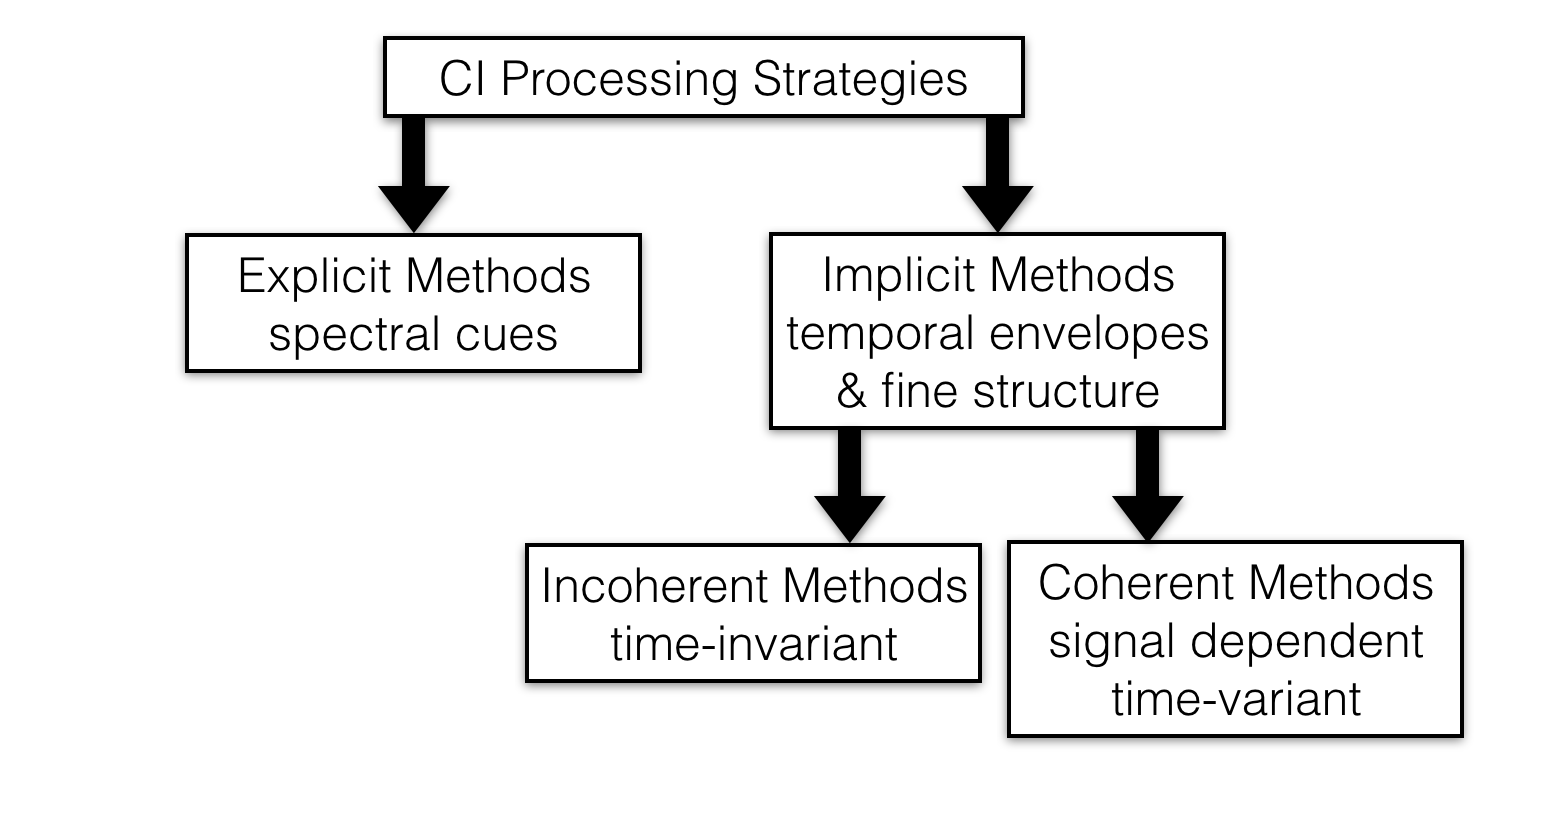
\includegraphics[width=.8\textwidth]{explicitVimplicit}   
    \caption{Classification Scheme for CI Processing Strategies}\label{fig:explicitVimplicit}
\end{figure}

A natural application of coherent processing is harmonic signals.  Harmonic signals are structured such that energy is focused in narrowband components centered around integer multiples of a fundamental frequency, denoted $F_0$.

Coherent processing has two possible advantages.  The first is the quality of features extracted, where quality means the reliability of extracted features with changes in the input.  For example, if the same note is played on two different instruments, same duration and volume, only the timbre should change.  It could be argued that to some extent this is a subjective measure, (psychoacoustic studies have shown that for $F_0$ differences of over an octave, there is a dependence of timbre perception on pitch \cite{marozeau2003dependency}), however within reasonable conditions there is a clear difference between perceptual changes dues to psychoacoustics and changes due to signal processing distortions.

The second advantage coherent processing may hold is the way in which features are transmitted to the cochlea.  Electric hearing has a much lower data rate than acoustic.  As a naive but simple explanation of this, consider that the cochlea has approximately 1500 hair cells transmitting information to the brain.  In contrast a typical cochlear implant has only 8-22 electrodes!  This clearly demands a data compression scheme.  Coherent processing can be used to intelligently select features in advantageous ways.

Quality of feature extraction and feature selection are two potentially independent benefits of coherent processing.  An incoherent method could extract distortion free envelopes, but then select which envelopes to transmit suboptimally.  Alternatively the envelopes selected could be the same as in a coherent method, however distortions are induced in the envelopes.

In this thesis, incoherent and coherent feature extraction methods are evaluated for the application of encoding harmonic signals.  The primary focus is on quality of feature extraction, however, some time is spent considering feature selection as well.

%\subsection{Why Harmonics?}

%we need a target for coherent processing

%harmonic signals are very common

%pitch discrimination is a major goal in CIs right now

%benefits to timbre, distinct talkers, etc.

%So why encode individual harmonics?  Well we have already discussed the benefits to processing, but what about the implications of encoding harmonic information?...


%So why encode individual harmonics?  The motivations fall into one of two general categories:  improved signal processing provided more knowledge of the input signal's structure or alternatively, improved perception because of harmonic representation.

% reduced artifacts, efficient data representation, stability
%Harmonics are linearly spaced in the frequency domain at multiples of a fundamental frequency, $F_0$.  Provided this fundamental frequency, which can be acquired via pitch estimation, an optimal system can be designed to extract features of individual harmonics.  It will be seen recurrently throughout this document that non-optimal systems induce distortions.

%timbre, pitch and rhythm are getting all the attention
%External to eliminating processing artifacts, a harmonic signal representation offers all the benefits that unique harmonic structures provide.  By definition, ``timbre is the perceptual attribute that distinguishes two sounds that have the same pitch, loudness, and duration'' (American National Standards Institute, 1973).  This primarily distinguishable as the unique onset times and amplitudes of individual harmonics.

%[Kang et al] developed a Clinical Assessment of Music Perception (CAMP) test in order to quantify music perception.  The two key dimensions they test are pitch and timbre.  Hybrid implants that provide simultaneous acoustic and electric hearing are a promising direction for pitch perception, however there are still no methods that get at the challenge of timbre perception.  The Harmonic Single Sideband Encoding strategy (HSSE), which has motivated this work, 


%improved pitch perception:
%``The general finding has been that place and rate coding in cochlear implants do not yield the same fine-grained pitch perception experienced by nor- mal-hearing listeners. This may in part be due to a complete lack of resolved harmonics in cochlear implants, as well as a lack of temporal fine structure coding—most current implants convey only tempo- ral envelope information and discard the temporal fine structure'' [oxenham]



%- Help differentiate signals, (timbre), improve SIN performance, free up channels for other information

%how harmonic?

%- redesign the envelope and fine structure encoding
%Many strategies consider the effects of leaving modulations in the signal, but nothing really talks about what the envelope should be, independent of the modulations.  If we do this first, we can then think about how the modulations affect this envelope as a separate modulation component.

%we are considering what is the ideal matched filter, and how close of an approximation do we need?


\section{Survey of Literature}

Separately, there is a great deal of research in cochlear implant processing strategies and harmonic signal processing, but there is limited literature that investigates the two together.

Harris \cite{harris1978use} investigated effects of discrete Fourier transform (DFT) window design on isolating harmonics in the presence of nearby strong harmonic interference.  Liguori et al. \cite{liguori2004intelligent} designed an intelligent fast Fourier transform (FFT)-analyzer that interpolates bins to minimize harmonic interference.  Alternative to DFT analysis, Li and Atlas \cite{li2003time} used an extended least-squares harmonic model to estimate harmonic features of a signal with time-varying $F_0$.

Nogueira et al. \cite{nogueira2005psychoacoustic} developed the MP3000 CI strategy which uses psycho-acoustic masking to more efficiently represent the same acoustic information.  Lai and Dillier \cite{lai2008investigating} investigated musical instrument discrimination with MP3000 and found no improvement over ACE.  This strategy can eliminate the redundant representation of a single harmonic, however the envelopes are extracted incoherently and suffer the same artifacts as ACE.

Laneau et al. \cite{laneau2006improved} proposed F0mod which explicitly modulates envelopes at a rate of $F_0$.  Improved pitch discrimination was observed for some conditions.  Vandali and van Hoesel \cite{vandali2011development} developed an enchanced-envelope-encoder (eTone) strategy that temporally modulates envelopes at a depth proportional to the harmonic probability, (probability the incoherent envelope is from a signal harmonic).  Furthermore, eTone attempts to coherently improve signal representation by biasing channel selection toward channels with higher harmonic probabilities.  Neither F0mod nor eTone attempt to modify the incoherent envelope extraction method of ACE.

Li et al. \cite{li2010harmonic} developed a harmonic single sideband encoder (HSSE) that uses a pitch estimator to coherently extract harmonic features.  Tests on music perception \cite{li2013improved} showed significant improvement on timbre recognition for CI users.


%"The HiRes120 strategy, used in the Advanced Bionics implant, is the first commercial stimulating strategy that uses the virtual channel technique. Virtual channels are created by adjusting the current level ratio of two neighboring electrodes."


%Equivalent noise bandwidth (ENBW) considers BW of noise if squished into a box of gain 1 around the downshift frequency.  [windows for harmonic analysis] This isn't entirely applicable since our harmonic has BW > epsilon, and since for any window most of the energy is close to 0, most of the so-called noise is actually desired harmonic signal.  If this were not the case, (I think) rectangular window would be the best, but since it distributes the noise more heavily to higher frequencies away from zero, it is actually worse (higher sidelobes)

%``some windows have a high rate of sidelobe decay that allows minimizing the error due to interference. However the steeper the sidelobe decay
%the wider the main lobe width and then the worse the minimum resolution bandwidth.'' [An Intelligent FFT-Analyzer with Harmonic Interference Effect Correction and Uncertainty Evaluation]

%``For NH listeners, the timbre space was best represented in three dimensions, one correlated with the temporal envelope (log-attack time) of the stimuli, one correlated with the spectral envelope (spectral centroid), and one correlated with the spectral fine structure (spectral irregularity) of the stimuli. The timbre space from CI listeners, however, was best represented by two dimensions, one correlated with temporal envelope features and the other weakly correlated with spectral envelope features of the stimuli. 
%``temporal envelope is dominant cue for timbre perception in CI listeners''
%[Temporal and Spectral Cues for Musical TimbrePerception in Electric Hearing]

%Hypothesis:
%--temporal envelope (log-attack time)
%this is in some cases smeared in time (F0mod) and in other cases mixed across harmonics
%--one correlated with the spectral envelope (spectral centroid)
%this is not as clearly represented as it could be (are we talking about resonance or per-harmonic details such as clarinet?)
%--one correlated with the spectral fine structure (spectral irregularity)
%this manifests in the envelope for CI processing, the problem though is that it is blurred across harmonics so the noise-like characteristics will be smoothed.

\section{Contents of Thesis}

This thesis is organized as follows.  In chapter~\ref{ch:ci_processing} background information and three relevant signal processing strategies are reviewed.  In chapter~\ref{ch:envelope_extraction} incoherent and coherent methods of signal analysis are compared.  In chapter~\ref{ch:harmonic_envelopes} a generalized coherent analysis method is applied to extraction of harmonic features.  Finally, chapter~\ref{ch:conclusion} takes into account practical implementation considerations and concludes this thesis.

\section{Notational Conventions}

In order to remain consistent throughout this document, the following notational conventions will be defined.  $F_0$ is fundamental frequency, $F_1$ is first harmonic, $F_1 = 2F_0$ and the $k$th harmonic is $F_k = (k+1)F_0$.

Specific conventions are itemized in the following list:

$j$ - the imaginary unit, $\sqrt{-1}$

$\mathcal{K}$ - number of envelopes per frame

$\mathcal{M}$ - number of electrode channels

$\mathcal{N}$ - number of electrodes stimulated per frame

$x[n]$ - a time series, (digitally sampled signal)

$x_k[n]$ - $k$th analytic subband of $x[n]$

$m_k[n]$ - envelope of $x_k[n]$

$c_k[n]$ - carrier of $x_k[n]$

$\mathcal{H}\{\cdot\}$ - Hilbert Transform

$\mathcal{F}\{\cdot\}$ - Fourier Transform

$\widehat{x}[n]$ - the Hilbert Transform of $x[n]$

$X(w)$ - discrete-time Fourier transform (DTFT) of $x[n]$

$X[k]$ - discrete Fourier transform (DFT) of $x[n]$

$X[n,w)$ - continuous-frequency short time Fourier transform (STFT) of $x[n]$

$X[n,k]$ - short time Fourier transform (STFT) of $x[n]$

$h[n]$ - filter impulse response

$\theta$ - angle

$\phi$ - phase

$f$ - frequency

% ========== Chapter 2

\chapter{Cochlea Implant Processing}\label{ch:ci_processing}

Human hearing is tonotopic, that is, starting in the cochlea and through the rest of processing in the brain, sounds far apart in frequency are processed separately.  The cochlea is spatially arranged; As a sound propagates through the basilar membrane the different frequencies are amplified or suppressed such that they stimulate locations physically far apart in the cochlea.

%"In spite of the fact that this analog signal itself preserves most of the original temporospectral information, the signal transfers to the auditory nerve is handicapped by the limited maximal firing frequency of the auditory nerve in response to the electrical stimulation. High synchronization of nerve fibers and the neural refractory period only allow for frequency transmission up to 1 kHz via temporal coding alone. For frequencies above 1 kHz, the spectral information cannot be sufficiently transferred by temporal coding alone. Multichannel implants have been developed to make use of the tonotopic organization in the cochlea and thus transmit more spectral information to the auditory nerve." \cite{somek2006coding}

In a cochlear implant an array of electrodes is inserted into the cochlea.  This array is intentionally designed to have a tonotopic organization.  When current is sent to the most deeply inserted (apical) electrodes, neurons associated with low frequency sounds are stimulated.  Conversely, current at a basal electrode will stimulate neurons associated with high frequencies.

Early cochlear implant strategies, under the category compressed-analog (CA), delivered band-specific analog signals to each electrode.  By using bandpass filters and an electrode array the implant emulates the tonotopic organization of acoustic hearing.

Current processing strategies use feature extraction to achieve much higher performance on speech recognition.  From each bandlimited signal a slow-time-varying envelope is extracted and the extra information is discarded \cite{vandali2005pitch}.  The envelopes are amplitude compressed and then used to modulate continuous bipolar pulse trains on each electrode channel.

These strategies all stem from an original parent, continuous-interleaved-sampling (CIS).  CIS is a solution to the problem of electric field interaction.  By interleaving pulse-trains there is minimal interaction between electrodes.


\begin{figure}[!ht]
  \centering
    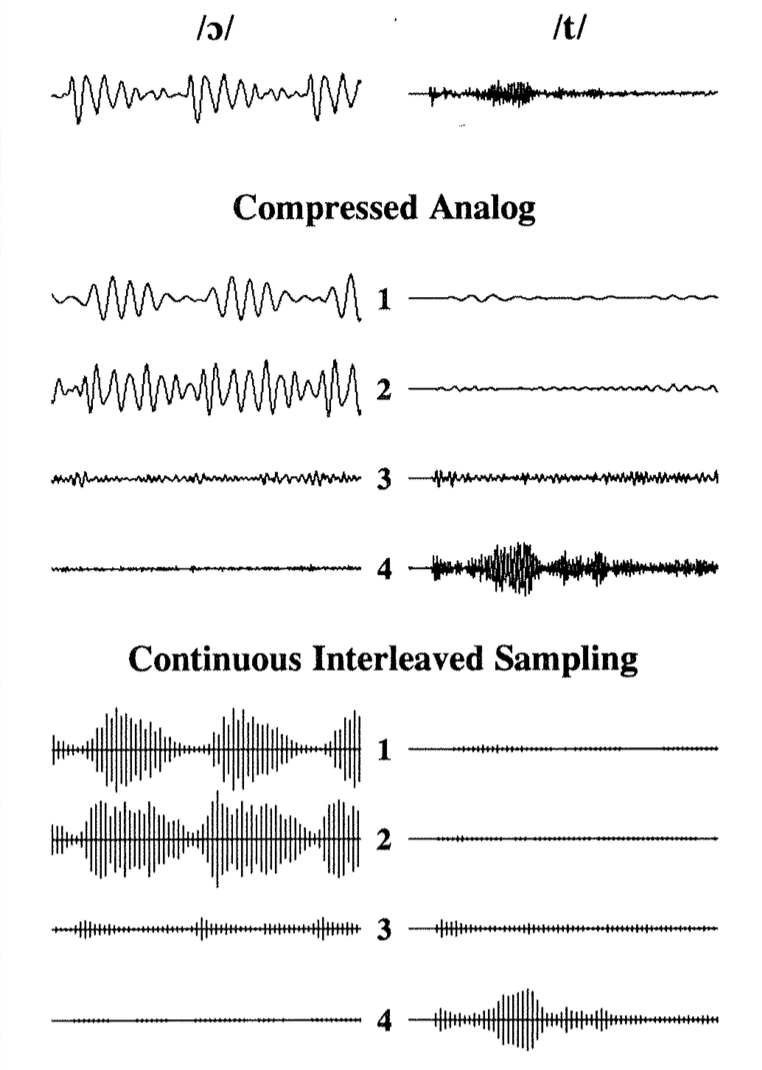
\includegraphics[width=.5\textwidth]{caVScis}   
    \caption{CA vs CIS}
\end{figure}

\subsection{Sum-of-Products Model}

We have now laid out enough background information to introduce a mathematical model for audio signals called the sum-of-products model.

In this model, a digitally sampled audio signal $x[n]$ is composed of bandpass components $x_k[n]$.  In each bandpass component a slow-time-varying envelope $m_k[n]$ multiplies a quickly-oscillating carrier $c_k[n]$.

\begin{align}
\label{eq:sum-of-products}
x[n] = \sum\limits_k x_k[n] = \sum\limits_k m_k[n] c_k[n]
\end{align}

Although there are infinite ways to decompose a signal into a sum-of-products, the model stems from real-word signals.  To gain some intuition consider, for example, a voiced vowel.  The vocal tract can be thought of as generating the carriers, $c_k[n]$.  Without changing the position of the mouth, one can change the pitch of a note.  The mouth then changes the temporal envelopes, $m_k[n]$.  As the mouth changes shapes it changes the formant structure structure.  Equivalently, it adjusts the relative amplitude of each bandpass component $x_k[n]$.

As another example, the pitch and timbre of musical instruments.  The pitch is characterized by the carriers but the timbre which is predominantly characterized by the attack time and spectral centroid \cite{kong2011temporal} will be encoded in the rise time and relative amplitude of the envelopes.

%``We begin by specifying the desired qualitative properties of the factors mk[n] and ck[n]. Generally, mk[n] is thought to represent the envelope, or slowly-varying temporal contour, of xk[n]. Conversely, ck[n] contains the quickly-oscillating fine structure of xk[n]. These designations lead to a convenient analogy with amplitude- and frequency- modulation systems in communications theory, which employ signal multipliers to convert low-frequency messages to high-frequency signals with better transmission characteristics. Along these lines, we assume xk[n] is of the form
%xk[n] = mk[n] · ck[n] = mk[n] · ejφk[n], (2.2)
%where ck[n] is the oscillating carrier and mk[n] is the low-frequency modulator, or message. Since the carrier is unimodular, all of the magnitude information about xk[n] resides in the envelope-like modulator.'' - clark thesis

%specify harmonic case of sum-of-products? this describes why coherent methods ... motivates coherent methods i guess

\subsection{Why Envelopes?}

One of the motivations for this approach is the limited ability to perceive temporal modulations in electric hearing.  In acoustic hearing modulations up to a few kHz may be perceptible, however cochlear implant envelope extraction techniques are designed to limit modulations, typically to around 160 to 320 Hz, which is closer to the range perceptible in electric hearing.

Modulation rates are also limited by pulse rate.  Although there isn't a quantitative value analogous to Nyquist rate, modulations at rates higher than a certain percentage of the constant pulse rate will not be represented accurately by the modulated pulse train.  That being said, cochlear implants today support modulations typically upwards of 2000pps (pulses per second), which should be sufficient provided modulations limited to about 320Hz.

\subsection{The Channel Vocoder}

To gain some intuition as to how and why CIS processing works, consider a closely related system, the channel vocoder.  Vocoding is a method of signal analysis and synthesis initially designed for audio data compression in telecommunication.  As of the mid 70's the vocoder has gained widespread familiarity via the music industry as a funky voice effect.  It is most well known for the signature robot voice heard in hits such as Kraftwerk's song ``The Robots'' or Styx's ``Mr. Roboto''.  In its application to music, the vocoder extracts the bandlimited envelopes of one source, (typically vocal), and applies them to each subband component of a second source.

What's interesting is that this second source can be essentially any arbitrary broadband signal and yet we still understand speech from the first source.  In this way the vocoder acts as a form of lossy data compression; the low data-rate envelopes are extracted and they may be later applied to, for example, white-noise.

This tells us that speech information is predominantly contained in the bandlimited envelopes, and thanks to the incredible robustness of speech to distortion, an estimated envelope is sufficient for speech comprehension.

%TODO 2 - make this pretty and add math
\begin{figure}[!ht]
  \centering
    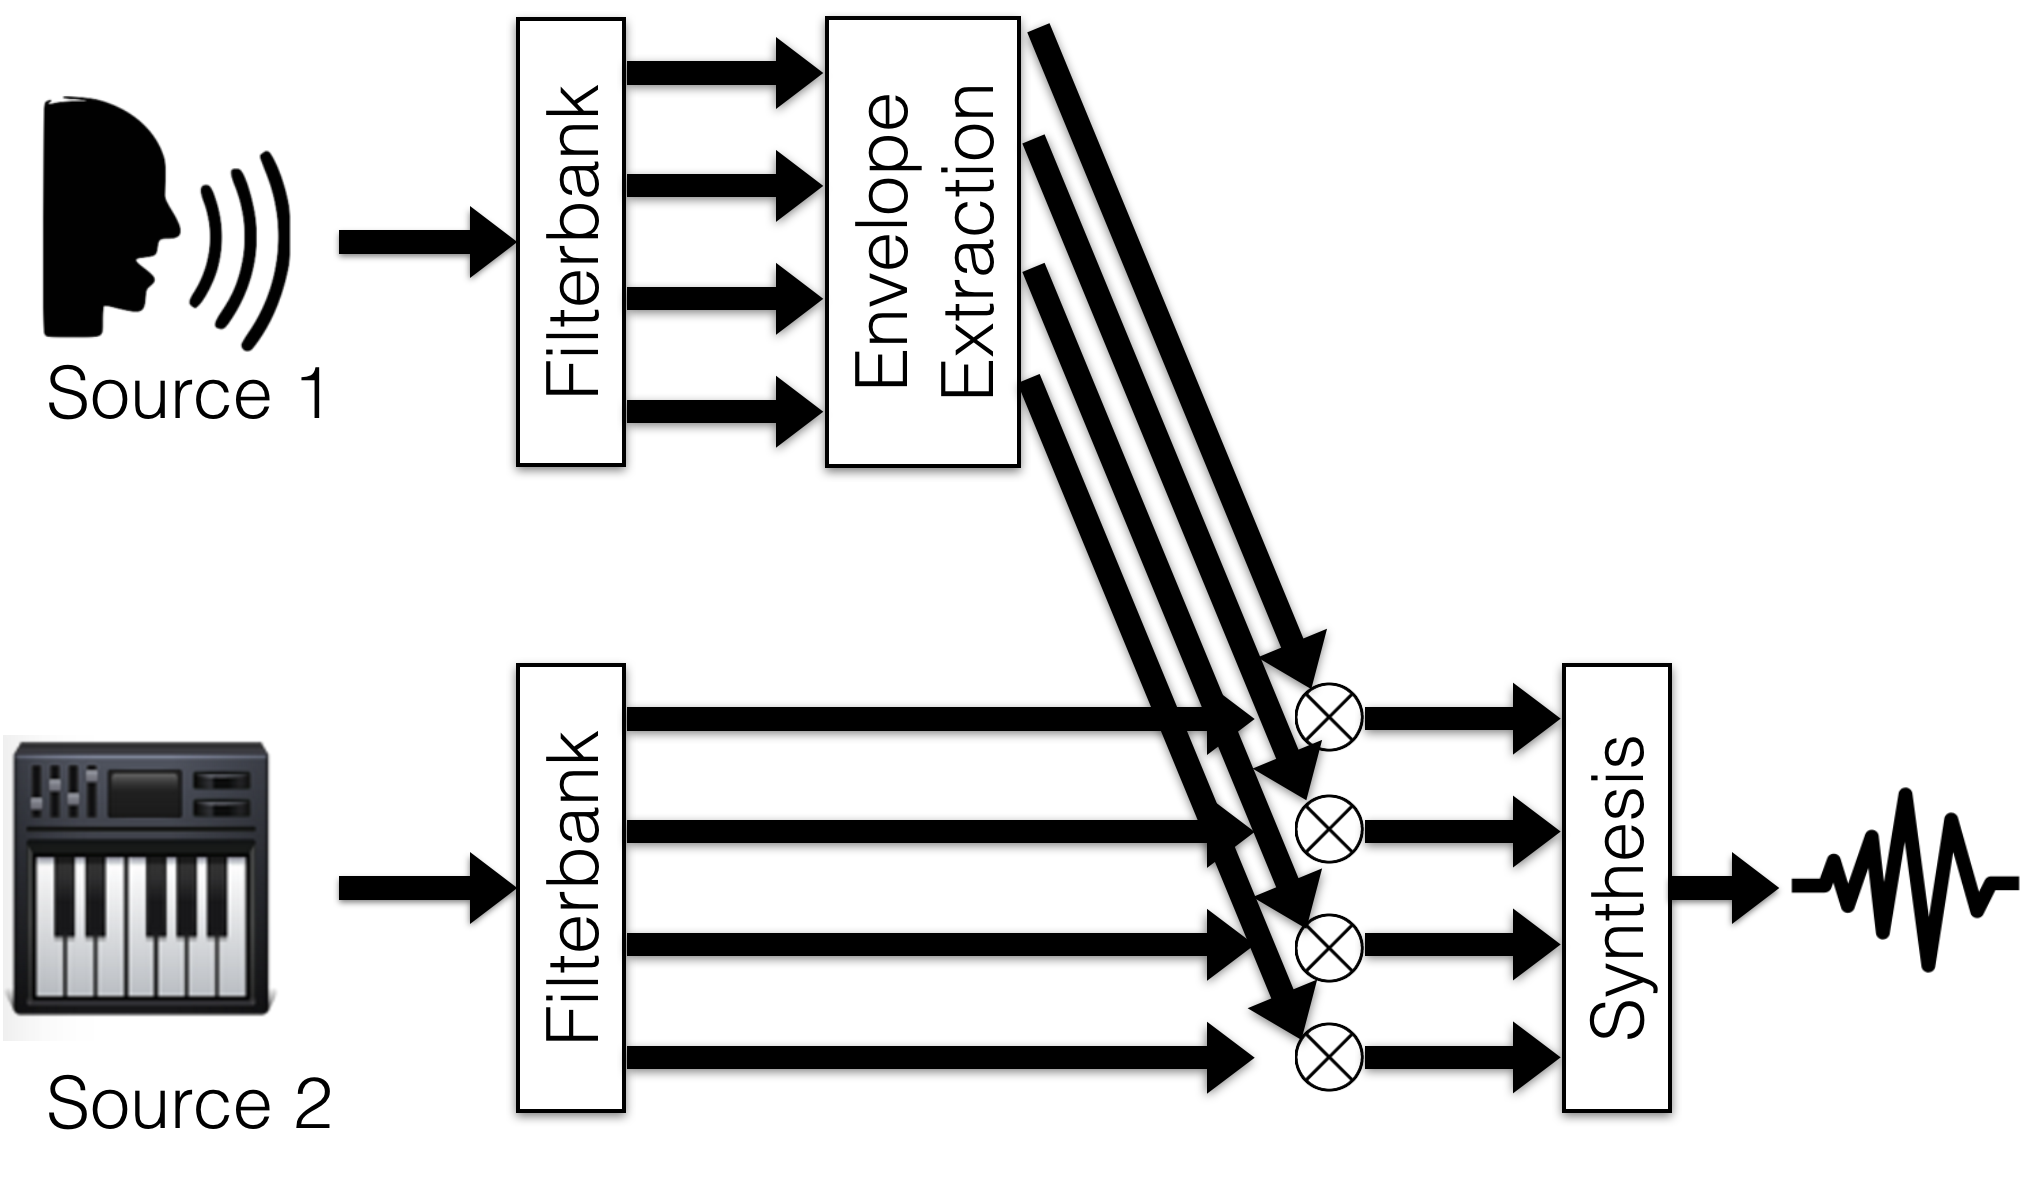
\includegraphics[width=.75\textwidth]{vocoder}   
    \caption{Channel Vocoder Processing}\label{fig:vocoder}
\end{figure}

It should be noted that the second source is typically chosen to be a broadband stationary signal.  If the signal is non-stationary it will have time-varying envelopes of its own which will interact with the envelopes of the first source. In terms of the sum-of-products model, the second source, $x^{(2)}[n]$, is a sum of time-invariant subbands and envelopes from the first source, $x^{(1)}[n]$ are applied.

\begin{align}
\label{eq:sum-of-products}
x^{(1)}[n] =& \sum\limits_k x_k^{(1)}[n] = \sum\limits_k m^{(1)}_k[n] c^{(1)}_k[n] \\
x^{(2)}[n] =& \sum\limits_k x_k^{(2)}[n] \\
y[n] =& \sum\limits_k m_k^{(1)}[n] x_k^{(2)}[n] 
\end{align}

Linking back, cochlear implant envelope extraction strategies do the same thing as vocoder signal analysis, as seen in figure~\ref{fig:vocoder}, however rather than using a second source to synthesize a new sound, the envelopes directly modulate electrical pulse trains.

\subsection{Temporal Fine Structure}

A major drawback to this method of encoding is the loss of temporal fine structure.  Recall that the extracted envelopes are transmitted and carrier information is discarded.

When using a vocoder, vocals sung at different pitches generate roughly the same output, $y[n]$.  Similarly in cochlear implants temporal fine structure that encodes pitch, as well as other signal characteristics, is lost in processing.

The previously statements don't paint the entire picture though.  Some temporal fine structure information may be transmitted if carrier information leaks into the estimated envelope.  Some strategies take advantage of this and intentionally allow for carrier leakage in the envelope.  ACE is an example of this approach.

% "Most cases with severe hearing loss involve damage to this conversion of a sound to an electric impulse in the cochlea. A cochlear implant bypasses this natural conversion process by directly stimulating the auditory nerve with electric pulses. Hence, the cochlear implant will have to mimic and replace auditory functions from the external ear to the inner ear." [trends inCI]

\subsection{Processing Blocks}

The main blocks of cochlear implants processing are visualized in figure~\ref{fig:CI_signal_flow}.  While at every stage adjustments can be made, for the purpose of comparing DSP algorithms, all other stages will be assumed constant throughout this work unless otherwise specified.

\begin{figure}[!ht]
  \centering
    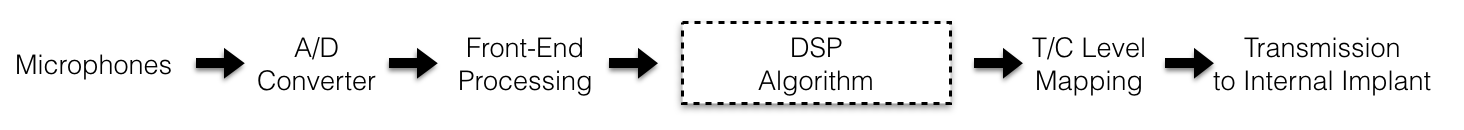
\includegraphics[width=1.0\textwidth]{CI_Signal_Flow}   
    \caption{Signal Flow in CI}\label{fig:CI_signal_flow}
\end{figure}

In this thesis, the output of the DSP stage will be a strictly positive signal used to amplitude modulate a constant bipolar pulse train.  T/C (threshold and comfort) Level Mapping is a logarithmically-compressed mapping from amplitude to current level.

\begin{figure}[!ht]
  \centering
    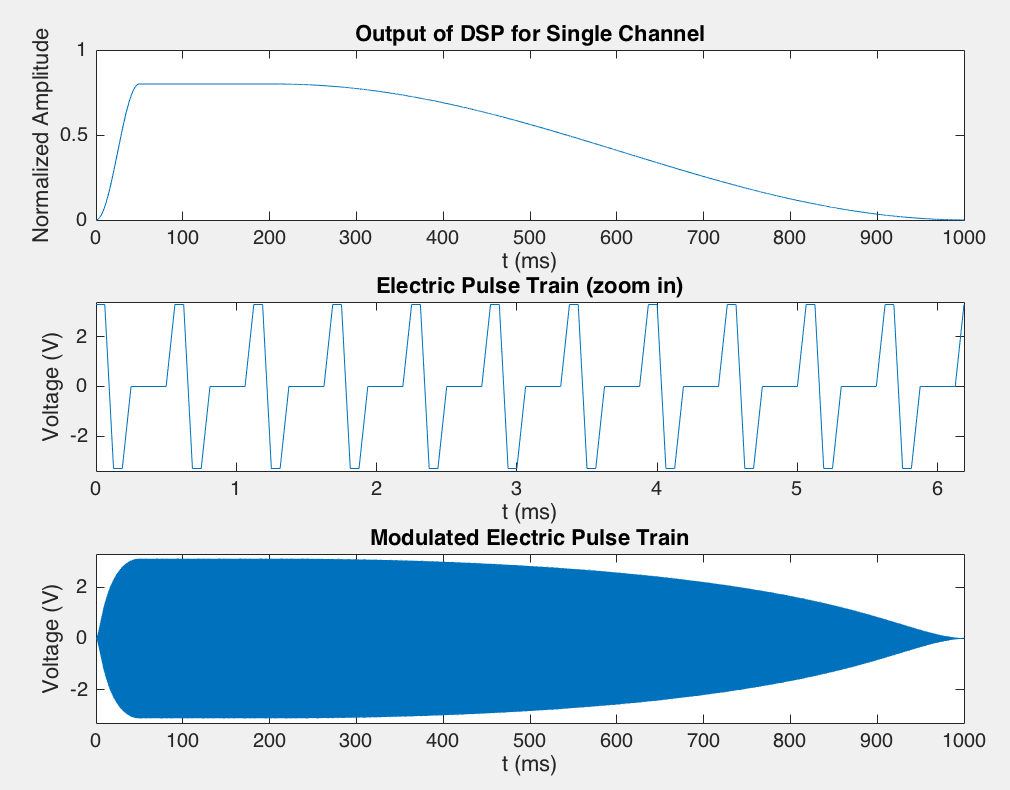
\includegraphics[width=1.0\textwidth]{output_of_dsp}   
    \caption{Tranformation from DSP output to Electrical Signal, the DSP output is compressed, then applied an electric pulse train to generate the final modulated electric pulse train}\label{fig:output_of_dsp}
\end{figure}

To summarize up to this point, a cochlear implants has an array of tonotopically organized electrodes.  On each electrode a electric pulse train is transmitted and that pulse train is modulated by a temporal envelope corresponding to a subband of the acoustic input signal.

\section{DSP Algorithms}

In order to gain insight into how to encode harmonic signals, in this section we will look inside the ``DSP Algorithm'' box; three specific strategies, ACE, F0mod, and HSSE will be compared with the goals of evaluating the pros and cons of each and considering how to optimize performance for harmonic encoding.

\subsection{ACE}\label{ss:ACE}

The simplest of the considered strategies is the Advanced Combination Encoder (ACE).  ACE is Cochlear Ltd's instance of the auditory community's generalized category of $\mathcal{N}$-of-$\mathcal{M}$ strategies.  In these strategies, $\mathcal{K}$ extracted envelopes are allocated to $\mathcal{M}$ channels corresponding uniquely to electrodes.  During each processing frame a subset, $\mathcal{N}$-of-$\mathcal{M}$, channel envelopes is selected for stimulation on the internal implant.  In the case that more than one envelope is allocated to a channel, the allocation stage must make a decision to select or combine envelopes in some way.

$\mathcal{K}$ - number of envelopes per frame

$\mathcal{M}$ - number of electrode channels

$\mathcal{N}$ - number of electrodes stimulated per frame

\begin{align}
\mathcal{K} \geq \mathcal{M} \geq \mathcal{N} \nonumber
\end{align}

A block diagram of ACE is visualized in figure~\ref{fig:ace_flow_diagram} and an equivalent condensed notation is shown in figure~\ref{fig:ace_flow_diagram_condensed}.  This condensed notation will be carried through to the other strategies analyzed.

%TODO 1 - change these figs to mathcal
\begin{figure}[!ht]
  \centering
    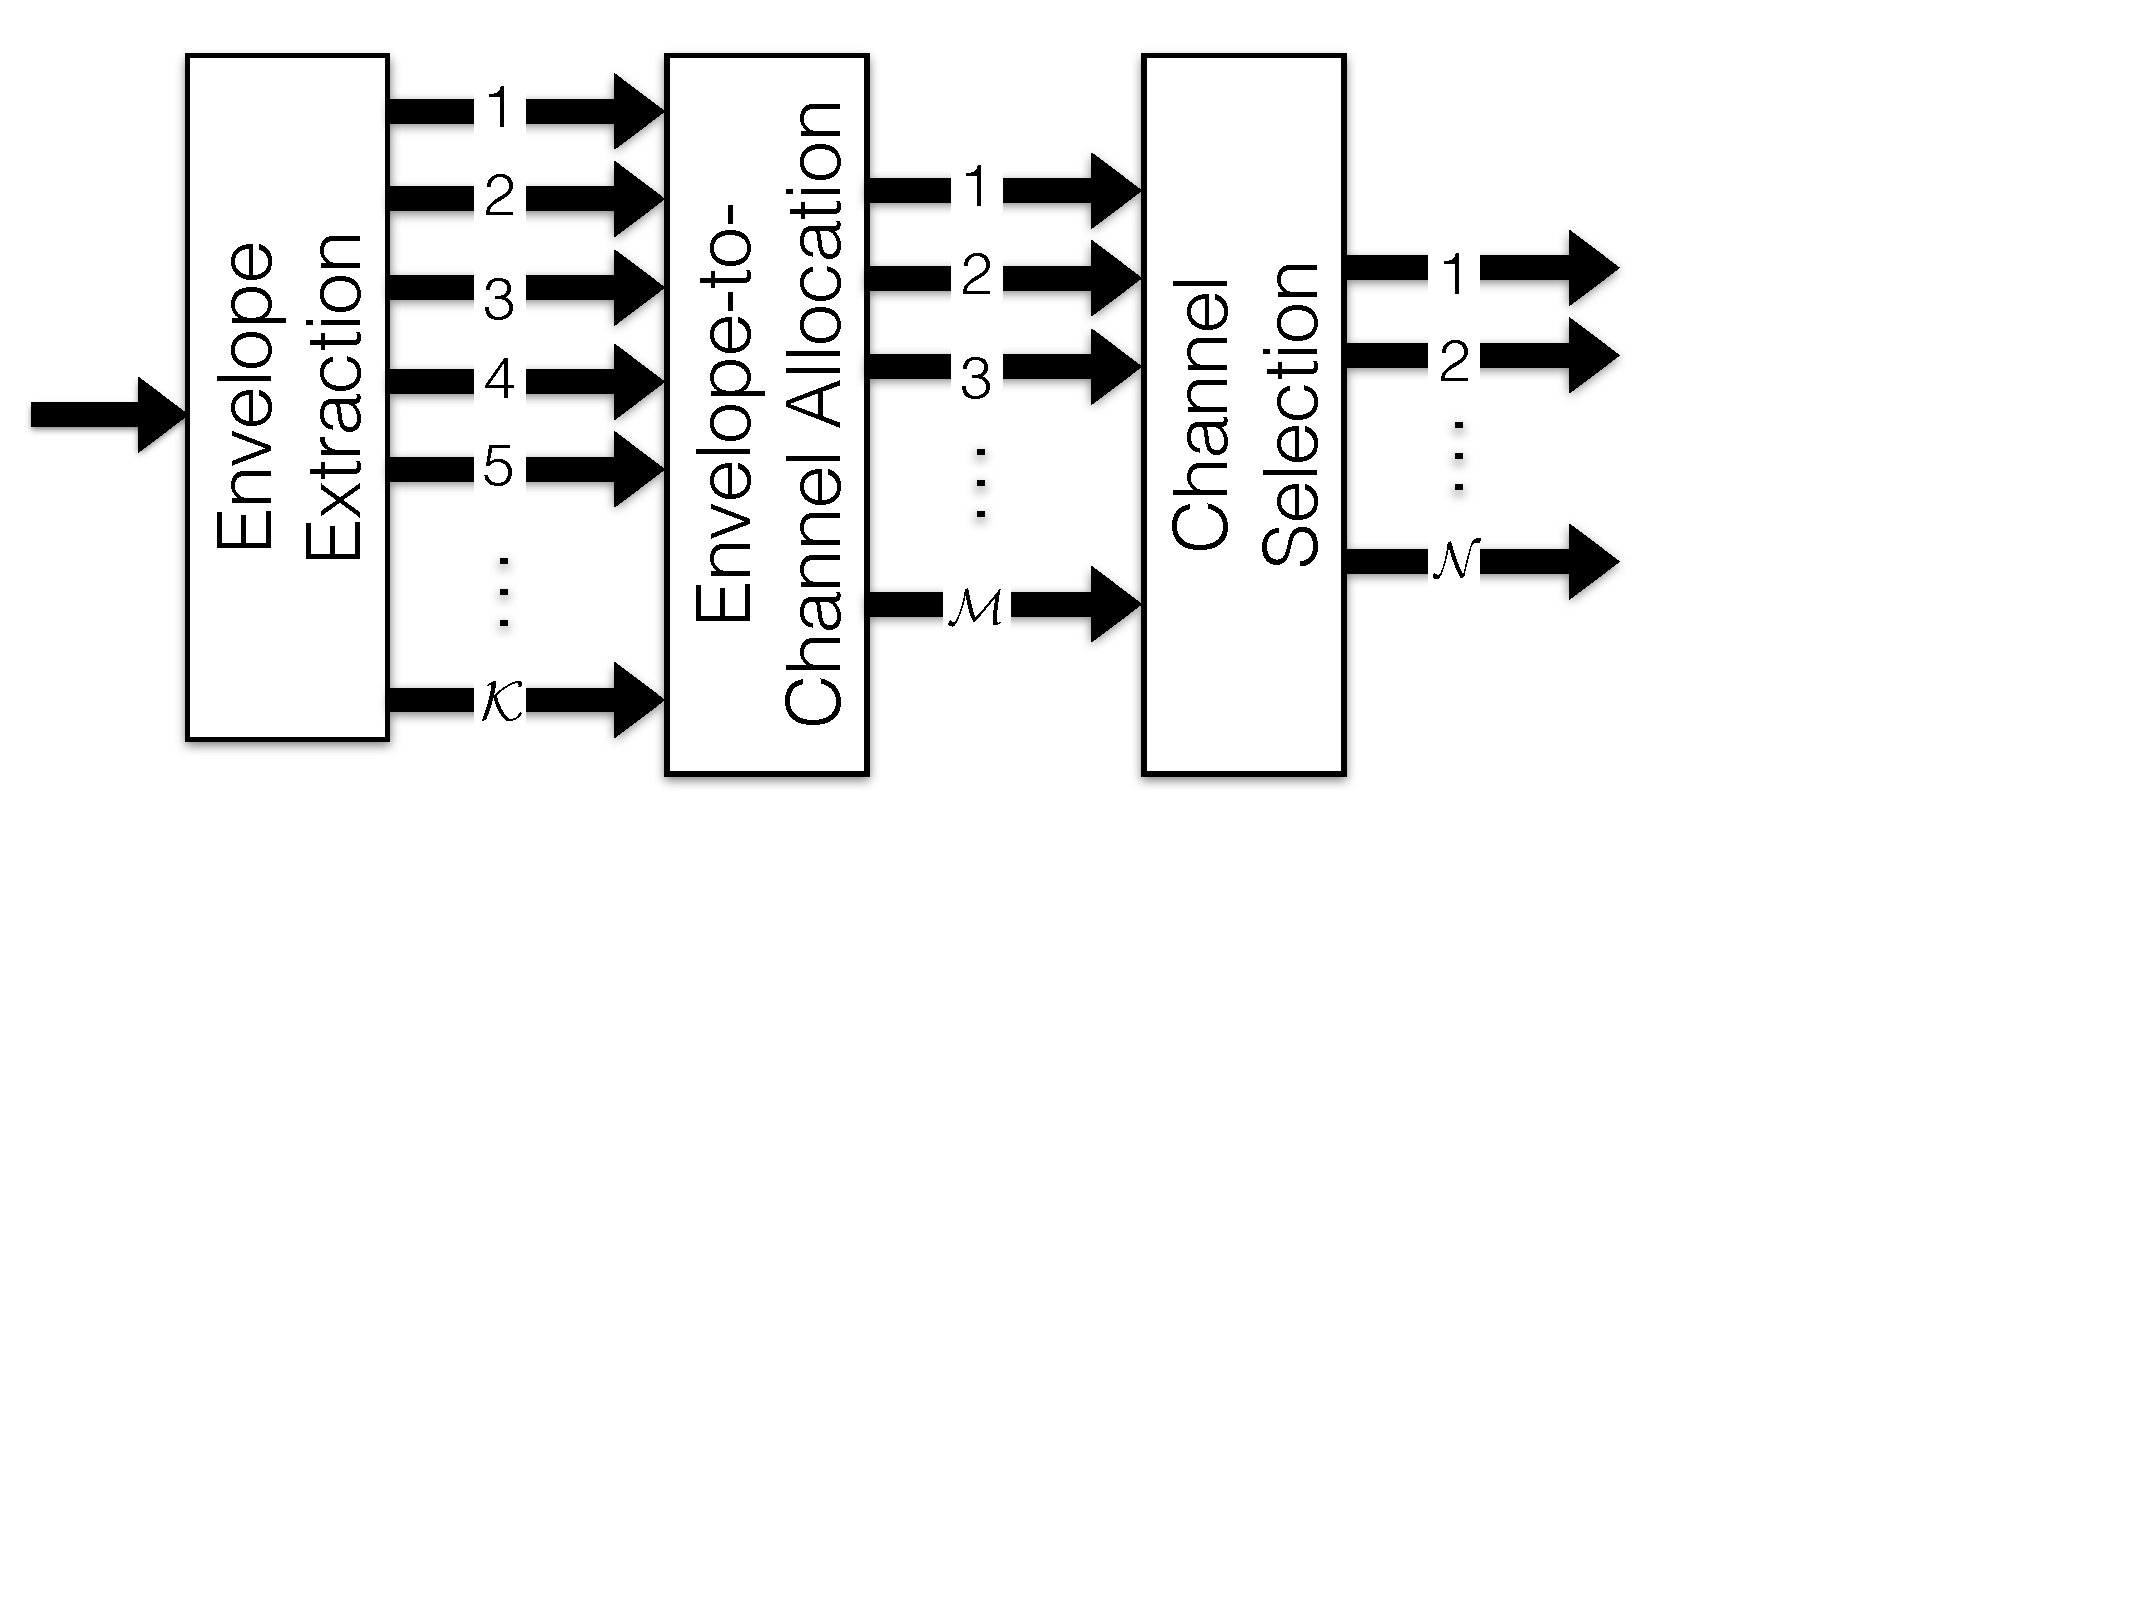
\includegraphics[width=0.5\textwidth]{ACE_flow_diagram_explicit}   
    \caption{ACE Flow Diagram}\label{fig:ace_flow_diagram}
\end{figure}

\begin{figure}[!ht]
  \centering
    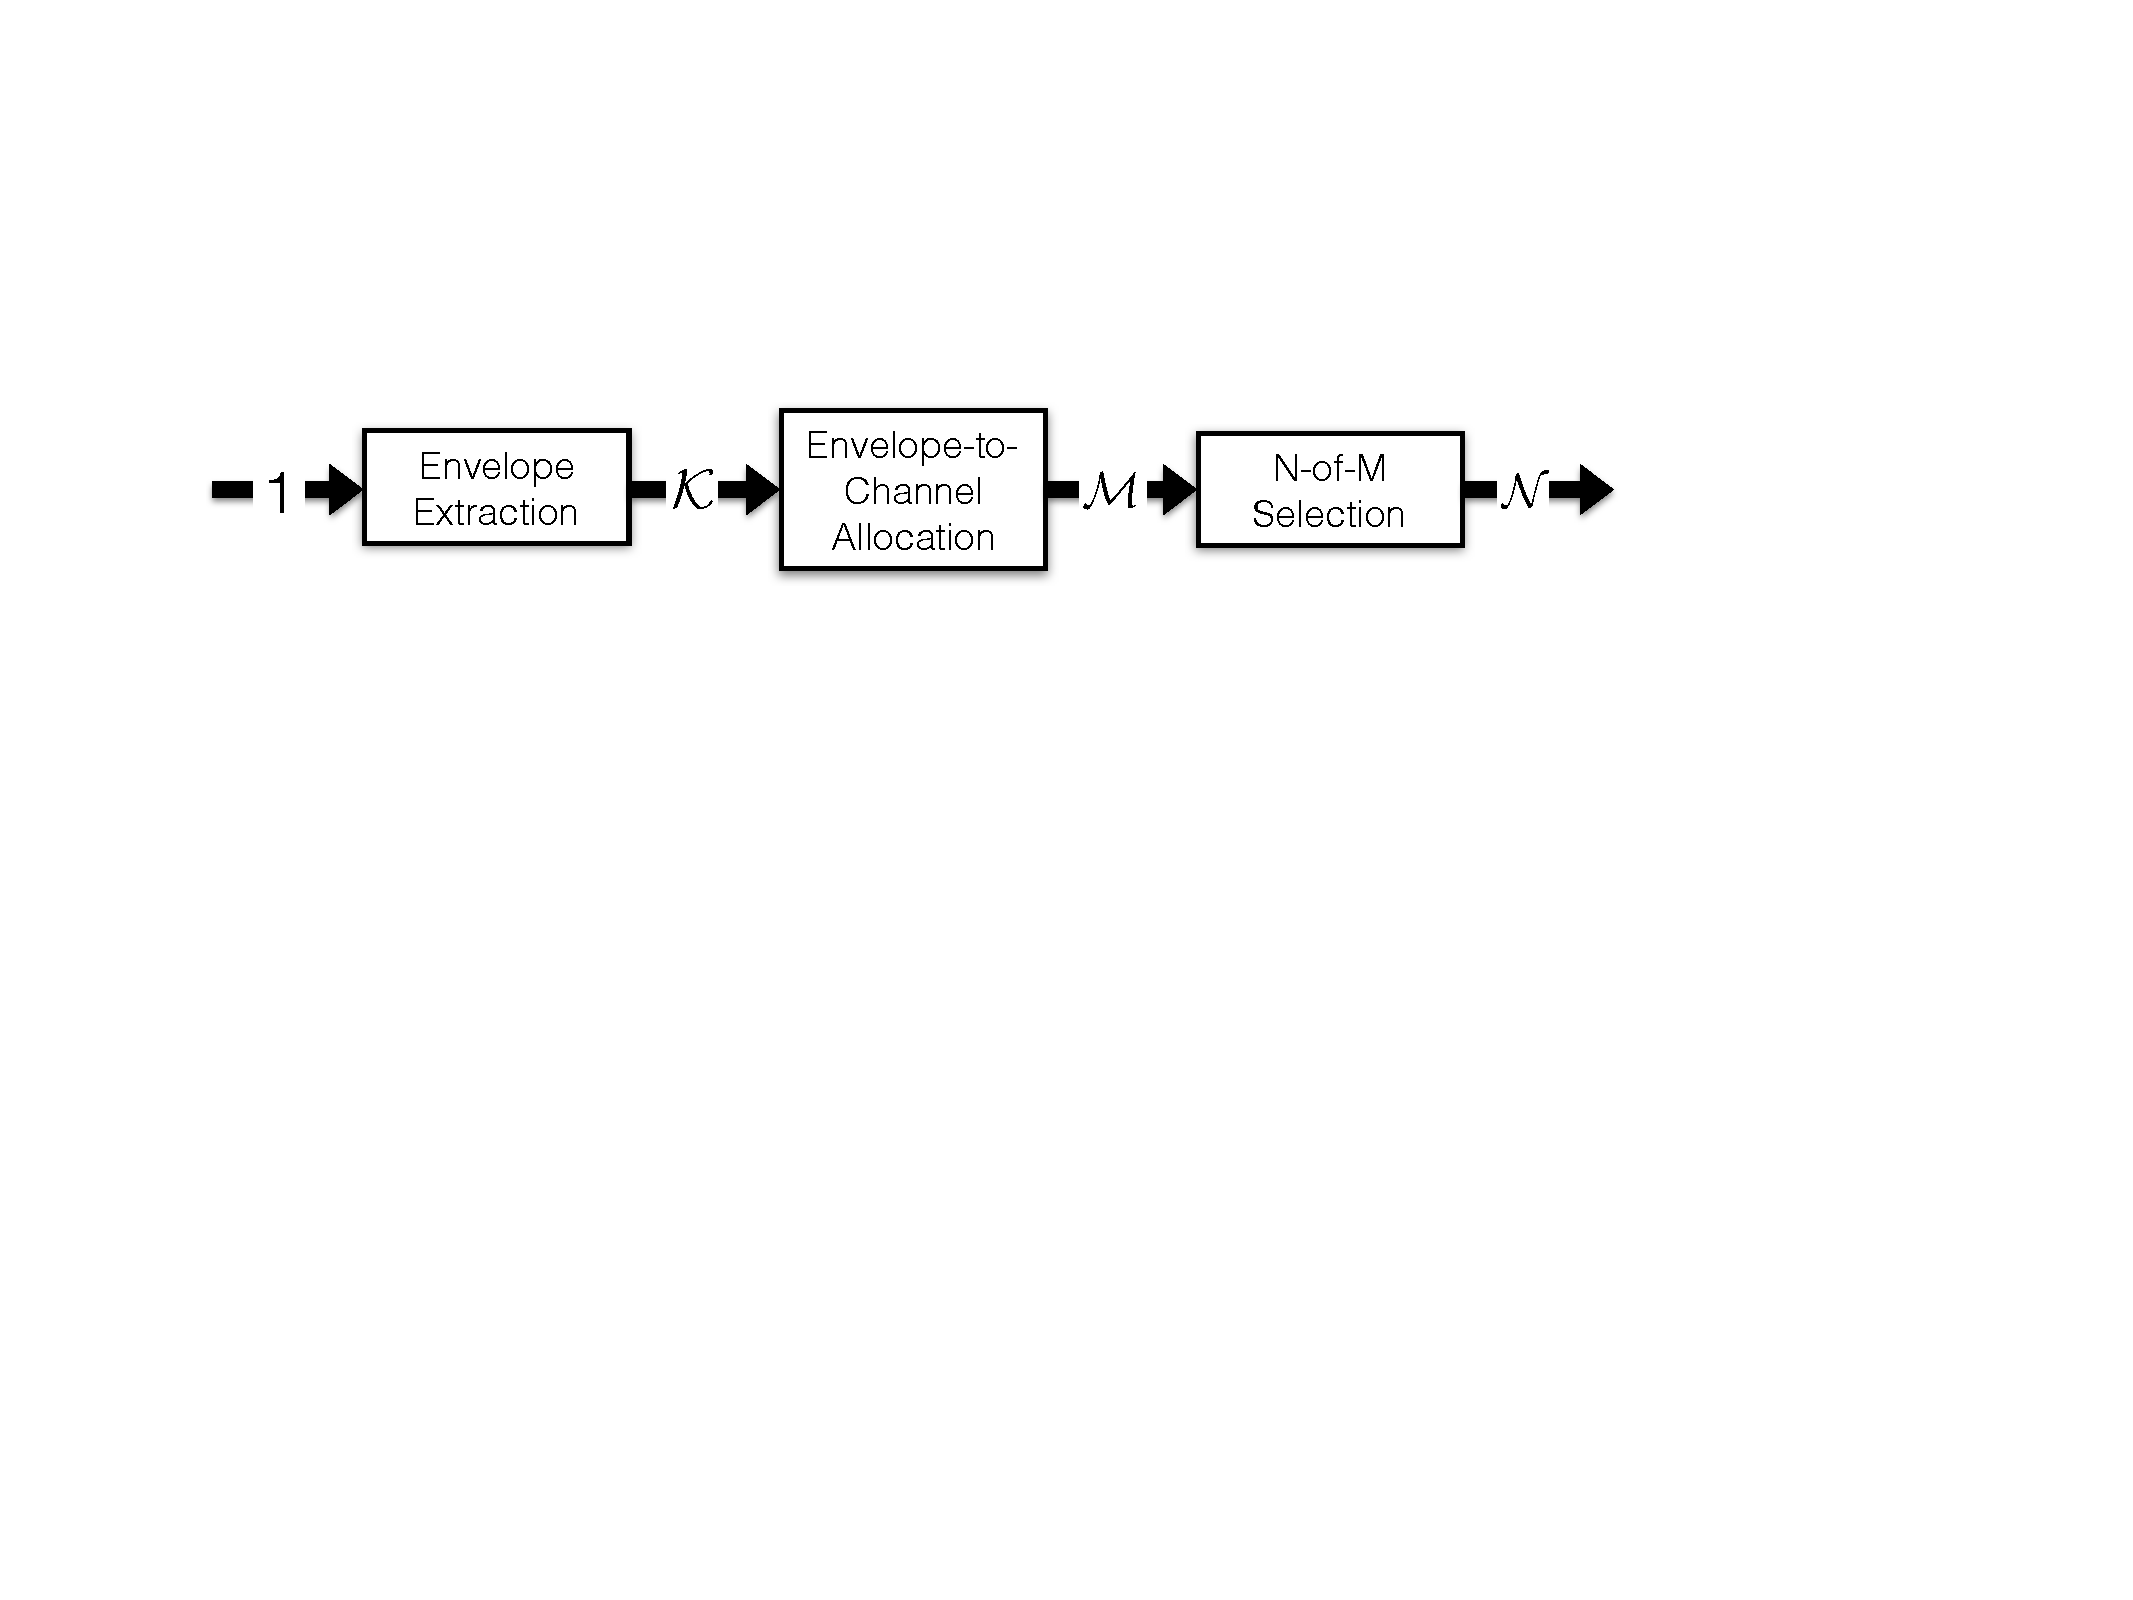
\includegraphics[width=1\textwidth]{ACE_flow_diagram}   
    \caption{condensed ACE Flow Diagram}\label{fig:ace_flow_diagram_condensed}
\end{figure}

While ACE does a sufficient job for many CI users in speech recognition tasks, a large gap remains between normal hearing and cochlear implants in many tasks such as pitch discrimination.  This is largely attributed to the lack of temporal fine structure information in this envelope encoding strategy.

%ACE uses place cues as the primary source of encoding a sound's characteristics.  To this day it is still unclear as to what implications this has.  This is due to a combination of factors including the subjective nature of pitch and absence of a ground truth baseline in many CI users.  For example, high-pass filtering a sound may cause it to sound brighter.  In contrast low-pass filtering would cause a warm quality.  As stimulus change electrodes a CI user could claim to experience changes in the high-low quality of pitch when really they are experiencing changes in the bright-warm quality of spectral distribution, or more likely an ambiguous combination of both.

%``Previous research had suggested that cochlear implant place pitch was more akin to brightness (an aspect of timbre) than to pitch. However, the Modified Melodies results supported the hypothesis that place pitch can support melody perception.'' [swanson thesis]

%There is general consensus that place cues are not sufficient for encoding pitch.  Alternatively, temporal cues encoded as time-domain carrier modulations have shown to be promising.

ACE does, however, provide limited temporal modulations via beat frequencies.  Through intentional processing artifacts, beat-frequencies will be induced in the processing of harmonic signals at a rate of the difference between the two harmonic frequencies, i.e. $F_0$.  Typically these modulations are not full depth and are usually limited to under 320Hz.

In this thesis, these artifact based modulations are termed induced modulations.  Looking at the flow diagram of figure~\ref{fig:ace_flow_diagram_condensed} it is not apparent that temporal modulations are contained in the processing path, however these modulations are encoded in the envelope itself.

Induced modulations are complementary to explicit modulations, used in F0mod and HSSE.  Explicit modulations are extracted from the signal separate from envelopes, and later applied to the final outputs.

\subsection{F0mod}

To get at the problem of pitch discrimination, Laneau et al. \cite{laneau2006improved} developed a new research strategy, F0mod.  F0mod provides the same processing as ACE with one important change, explicit carrier modulation.  It achieves this by adding a pitch estimator into the processing.

Once a fundamental frequency is acquired, all output envelopes are modulated by a raised sinusoid at a rate of $F_0$.  $F_0$ is used because of the limitations on ability to perceive high modulation rates with a CI.

\begin{figure}[!ht]
  \centering
    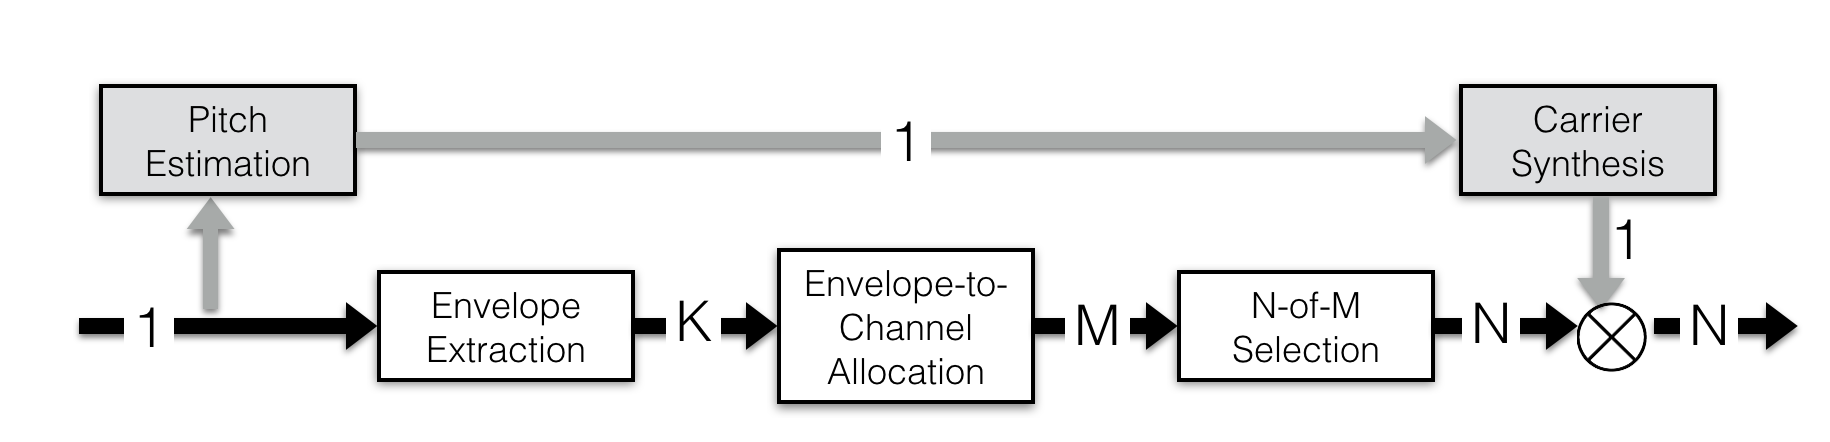
\includegraphics[width=1\textwidth]{F0mod_flow_diagram}   
    \caption{F0mod Flow Diagram}
\end{figure}

This raised sinusoid, defined in (\ref{eq:raised_sinusoid}), is constant modulation depth, (full dynamic range), and same across channels, (phase aligned).  An example comparing this to induced modulations is shown in figure~\ref{fig:induced_vs_explicit}.

\begin{align}
\label{eq:raised_sinusoid}
c[n] = 0.5 + 0.5cos(2\pi F_0n)
\end{align}

\begin{figure}[!ht]
  \centering
    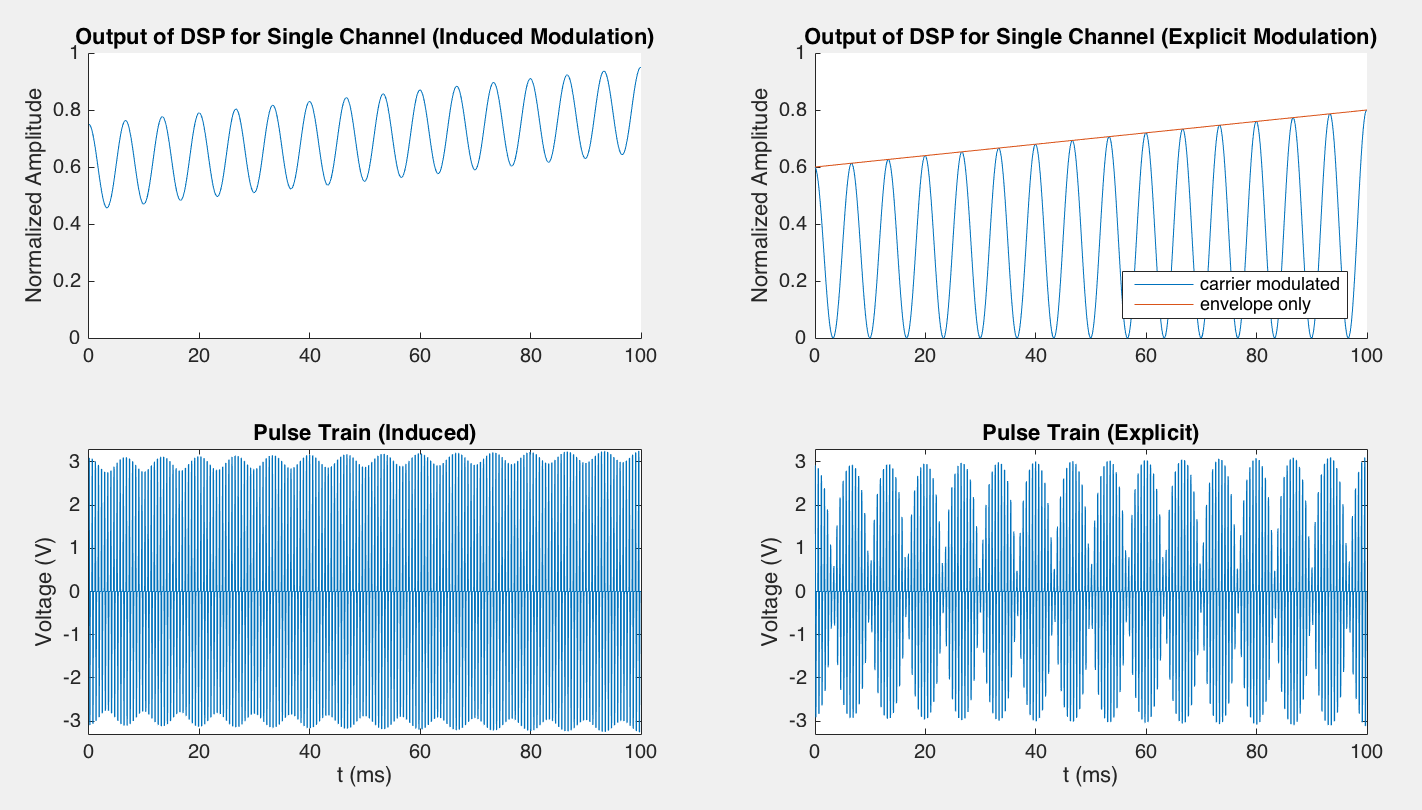
\includegraphics[width=1\textwidth]{induced_vs_explicit}   
    \caption{Induced vs Explicit Temporal Modulations Example}\label{fig:induced_vs_explicit}
\end{figure}

\subsection{HSSE}

Looking for a novel approach to improved pitch perception and, more broadly, music perception, Li et al. \cite{li2010harmonic} developed Harmonic Single Sideband Encoder (HSSE).  There are two different versions of HSSE.  We will start by describing the version most similar to F0mod.

In this version, coherent demodulation extracts harmonic envelopes.  These harmonic envelopes are then combined into channels based on the harmonic index and $F_0$.  Just as in F0mod a subset is selected for stimulation and then these envelopes are combined with carrier modulators.

\begin{align}
\mathcal{K}, \mathcal{M} \geq \mathcal{H} \nonumber
\end{align}

\begin{figure}[!ht]
  \centering
    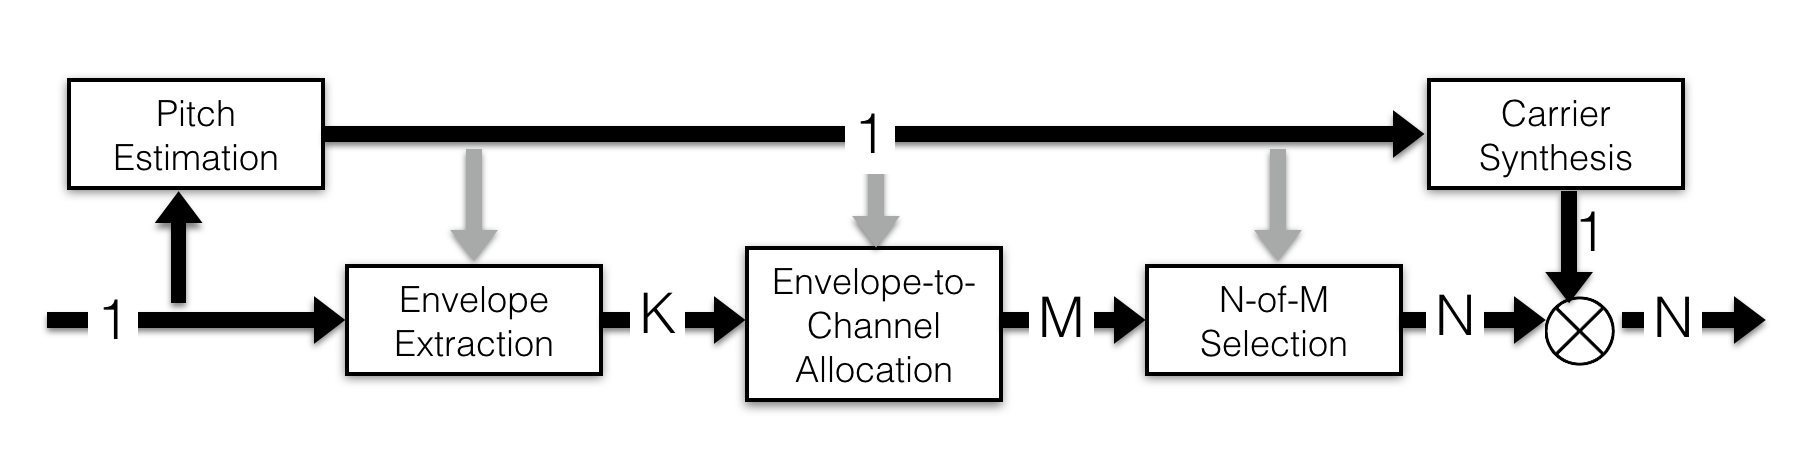
\includegraphics[width=1\textwidth]{HSSE_flow_diagram_noPhase}   
    \caption{HSSE Flow Diagram}\label{fig:HSSE_flow_1}
\end{figure}

The key differences between this and F0mod can be summarized quite simply: every stage of typical ACE processing is now done coherently using $F_0$ information.

It should be noted that it is not necessarily true that $\mathcal{K} \geq \mathcal{M}$.  In the case that no envelopes are allocated to a channel that channel is  ruled out during the selection stage.

In the second version, more information about the carriers is retained than just the fundamental frequency.  This puts some restrictions on the type of carrier than can be used, however it encodes time varying phase information which is unique to each envelope.

Because of the unique characteristics of each carrier, the carrier synthesis block must be moved to an earlier point in the processing.  First, complex envelopes containing phase information are extracted.  These envelopes are then combined with a common carrier at a rate of $F_0$, however, each output, which we will call a modulator, will be unique and time-varying in both magnitude and phase.  This version, which will be termed HSSE with coherent phase encoding, is visualized in figure~\ref{fig:HSSE_flow_2}

\begin{figure}[!ht]
  \centering
    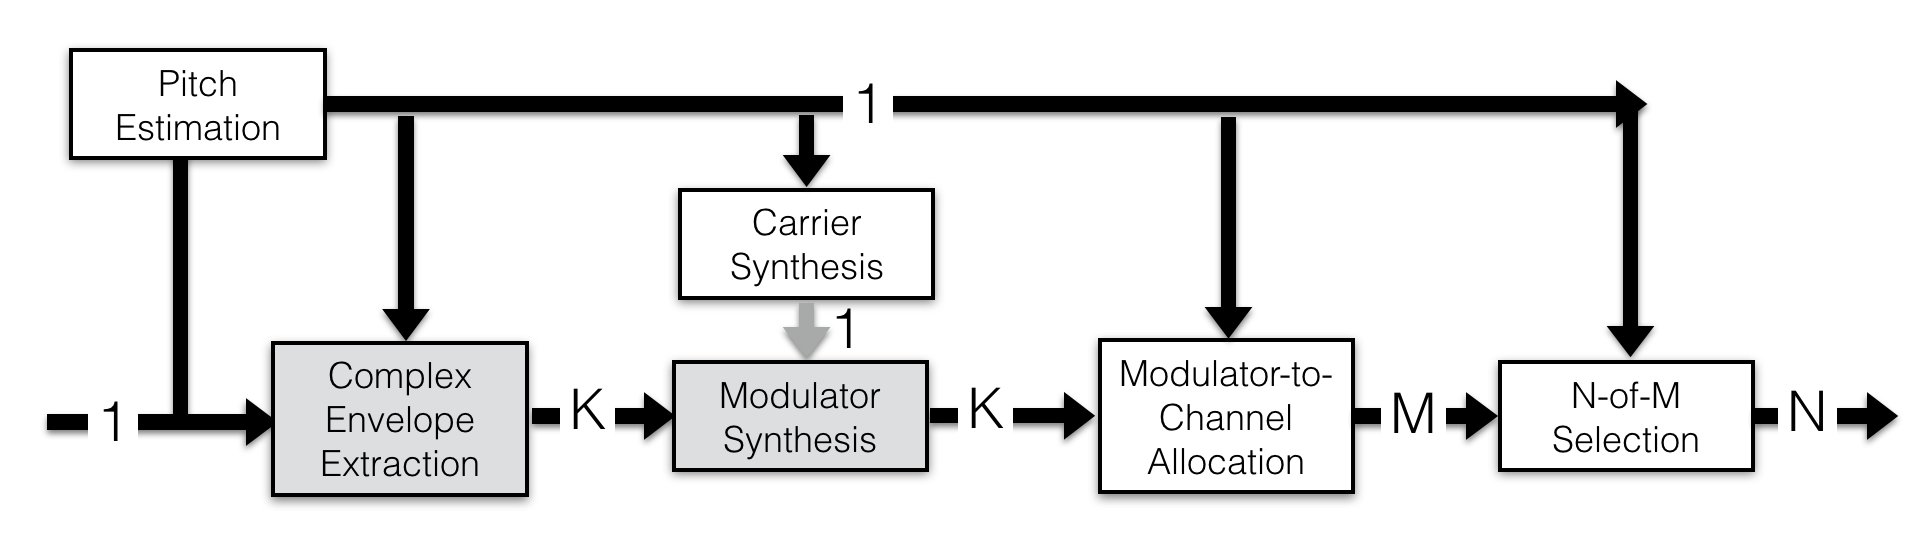
\includegraphics[width=1\textwidth]{HSSE_flow_diagram_Phase}   
    \caption{HSSE (with coherent phase encoding) Flow Diagram}\label{fig:HSSE_flow_2}
\end{figure}

\subsection{Summary}

Comparing these strategies, the differences may be summarized as:

%TODO 3 - make this pretty

1) Envelope Extraction Method (not discussed yet)

2) Temporal Encoding Method

a) induced vs explicit

b) phase encoding (explicit only)

c) modulation waveform (explicit only)

3) Envelope-to-Channel Allocation and Channel Selection

We will start by investigating 1 and 2(a,b).  Some considerations for 2(c) and 3 will be brought up upon concluding this thesis, however, the primary focus will be on 1 and 2(a,b).

Chapter~\ref{ch:envelope_extraction} will discuss mathematical methods to envelope extraction as well as phase preservation since phase is extracted at the same time.  As a result we will generalize 1 and we will answer 2(b).  Chapter~\ref{ch:harmonic_envelopes} will evaluate design considerations for 1 and in doing so, answer 2(a).  Chapter~\ref{ch:conclusion} will briefly discuss 2(c) and 3.

% ========== Chapter 3

\chapter{Envelope Extraction Methods}\label{ch:envelope_extraction}

This chapter will define the methods used to extract bandlimited temporal envelopes.  These methods fall under a general signal processing category of analysis-synthesis systems.  A signal is decomposed into its envelopes and carriers.  Then the envelopes and/or carriers are manipulated individually before recombination. 

One of the major focuses of research in this area is the evaluating the amount of distortion induced by the system.  For example, Ghitza's test is a way of measuring the out-of-band distortion of a modulation filtering system \cite{ghitza2001upper}.

Cochlear implant processing is a special case in that the final output is not an audio signal.  This means that only the first half, the analysis step, is applicable.  This is critical to understand when considering methods, as all of the considerations related to synthesis or full-system distortion are no longer relevant.

This chapter is organized as follows.  First, the incoherent and coherent envelope extraction methods will be defined.  Then an aside will be taken to consider the efficacy of coherent phase encoding.  Finally the extraction methods will be compared and a generalization defined.

\section{Incoherent Methods}

The difference between incoherent and coherent is actually quite simple.  Consider a system $T\{\cdot\}$.  If the system is time-invariant then it is incoherent.  If it is time-varying and the way in which it varies is a function of the input, it is called a coherent system.  This is visualized in figure~\ref{fig:incoherent_vs_coherent}.  In coherent methods the input not only passes through the system, it changes the system.

%TODO 1 - change H to T
\begin{figure}[!ht]
  \centering
    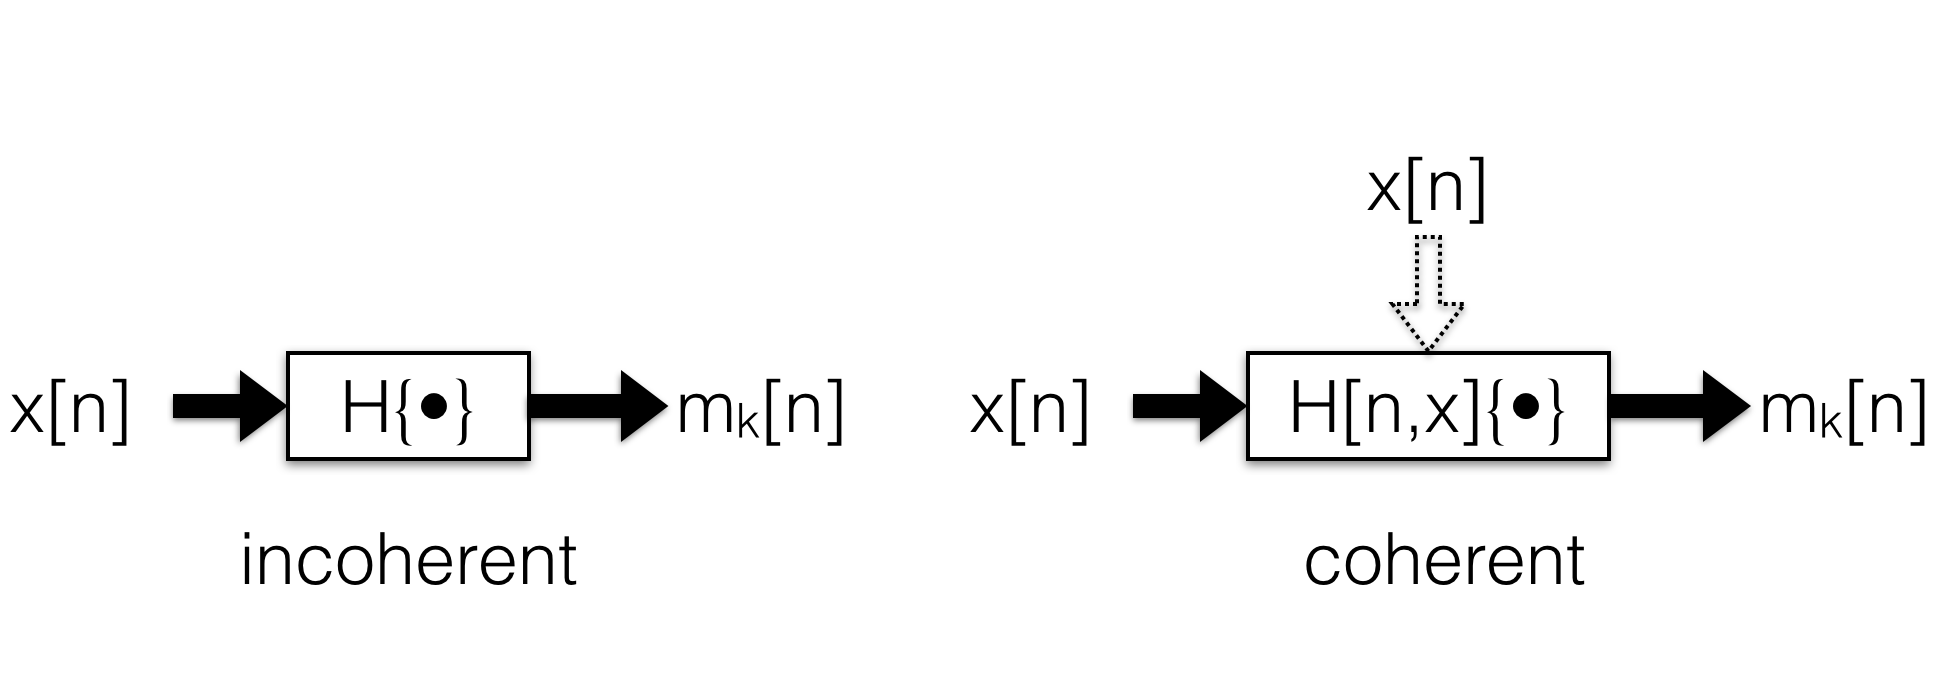
\includegraphics[width=1\textwidth]{incoherent_vs_coherent}   
    \caption{Incoherent vs Coherent Envelope Extraction}\label{fig:incoherent_vs_coherent}
\end{figure}

In all considered methods, the input is a real digitally sampled audio waveform, $x[n]$ bounded in the normalized range $[-1, 1]$.  For incoherent methods the output will be $\mathcal{K}$ real digital waveforms, $m_k[n]$, in the range $[0, 1]$.  All filters considered will be finite impulse response (FIR).

\subsection{Continuous Interleaved Sampling (CIS)}

This is method is specifically implemented by the CIS strategy.  The input is first bandpass filtered, where $h_k[n]$ is a bandpass filter and $k$ has arbitrary limits.  The subband is then full-wave rectified, (magnitude operation), and lowpass filtered.  $h_{lp}[n]$ is a lowpass filter, typically with a cutoff around 200-400Hz.

\begin{align}
m_{k,CIS}[n] =& \Big| x[n] * h_k[n] \Big| * h_{lp}[n]
\end{align}

In this method the number of filters is usually the same as the number of electrodes, $\mathcal{M} \approx 8$ to $22$, making $\mathcal{K}$ to $\mathcal{M}$ a one-to-one mapping.  These filters are thus non-uniform bandwidth and center frequency, with increasing bandwidth and wider spacing at higher frequencies.

\subsection{Hilbert Envelope}

The Hilbert envelope is a method of decomposition applied far more broadly than the field of cochlear implants.  Despite only retaining the envelope, we look at the carrier to gain insight as to how the signal $x[n]$ is represented in the decomposition.  The analytic bandpass signal, $x_k[n]$ is computed as \ref{eq:hilbert_transform}.  The envelope is defined as the magnitude, (\ref{eq:hilbert_envelope}).

\begin{align}
\label{eq:hilbert_transform}
x_k[n] =& x[n] * h_k[n] + j\mathcal{H}\{x[n] * h_k[n]\} \\
\label{eq:hilbert_envelope}
m_{k,hilbert}[n] =& \Big| \widehat{x}_k[n] \Big| \\
c_{k,hilbert}[n] =& cos(\angle\widehat{x}_k[n])
\end{align}

Intuitively, if the filterbank $\Big[h_1[n], h_2[n], ...,h_\mathcal{K}[n]\Big]$ has a flat total response, all of the information of the original signal is contained in the envelopes and carriers, and thus it is possible to reconstruct the input.

\subsection{Short Time Fourier Transform (STFT)}

The short-time Fourier transform (STFT) is not commonly associated with envelope extraction with respect to its prevalence in signal processing, however through analysis we will see that it fits the sum-of-products model.

The STFT has two classic interpretations: a series of windowed Fourier transforms, each at a different time instant, or a collection of uniform bandpass filters, each at a different center frequency.  The latter is more directly applicable to envelope extraction.

An STFT bin at discrete time $n$ and discrete frequency $k$ is defined as

\begin{align}
\label{eq:STFTdefinition}
X[n,k] = \sum\limits_{r=-\infty}^{\infty} x[r] w[r - n] e^{-j\frac{2\pi}{N}kr}, \qquad 0 \leq k < N
\end{align}

where $N$ is the DFT order, not to be confused with electrodes stimulated per frame, $\mathcal{N}$.  Defining a new variable $r' = r - n$ and defining the window such that  $w[n] = 0$ for $n < 0$ or $N \leq n$,

\begin{align}
X[n,k] =& \sum\limits_{r'=0}^{N-1} x[n + r'] w[r'] e^{-j\frac{2\pi}{N}k(n + r')} \nonumber \\
=& e^{-j\frac{2\pi}{N}kn} \sum\limits_{r'=0}^{N-1} x[n + r'] w[r'] e^{-j\frac{2\pi}{N}kr'}.
\end{align}

Let $X[n,k]$ be represented in polar form as

\begin{equation}
X[n,k] = \vert X[n,k]\vert e^{j\angle X[n,k]}.
\end{equation}

Assuming the window $w[n] \neq 0$ for $0 \leq n \leq N-1$ the inverse may be solved as

\begin{align}
\label{eq:hop_factor}
x[n + r'] =& \frac{1}{Nw[r']}  \sum\limits_{k=0}^{N-1} X[n,k] e^{j\frac{2\pi}{N}k(n+r')} \nonumber \\
=& \frac{1}{Nw[r']}  \sum\limits_{k=0}^{N-1} \vert X[n,k]\vert e^{j(\frac{2\pi}{N}k(n+r') + \angle X[n,k])} \\
\label{eq:hop_factor_1}
x[n] =&\sum\limits_{k=0}^{N-1}  \frac{1}{Nw[0]}  \vert X[n,k]\vert e^{j(\frac{2\pi}{N}kn + \angle X[n,k])}
\end{align}

(\ref{eq:hop_factor}) simplifies to (\ref{eq:hop_factor_1}) when the STFT hop-factor is one sample, which can be assumed without loss of generality.  For greater hop factors the inverse can always be computed from (\ref{eq:hop_factor}).  Of course, if the hop factor is greater than $N$ the original signal cannot be fully reconstructed.  This is especially noted because the factor $w[0]$ will be seen recurrently throughout this thesis.

The sum-of-products becomes clear in (\ref{eq:hop_factor_1}).

\begin{align}
\label{eq:envelope_STFT}
m_{k,STFT}[n] =  \frac{1}{Nw[0]}  \vert X[n,k]\vert \\
c_{k,STFT}[n] = e^{j(\frac{2\pi}{N}kn + \angle X[n,k])}
\end{align}

The STFT can be thought of as a series of $N$ linear time-invariant (LTI) systems that each downshift the input signal, then lowpass filter.  This can be seen mathematically by rewriting (\ref{eq:STFTdefinition}) as

\begin{align}
X[n,k] =& \sum\limits_{r=-\infty}^{\infty} x[r] e^{-j\frac{2\pi}{N}kr} w[-(n - r)] \nonumber \\
\label{eq:STFTasFilter}
=& x[n] e^{-j\frac{2\pi}{N}kn} * w[-n].
\end{align}

The STFT envelope has a similar form to the other methods after plugging (\ref{eq:STFTasFilter}) into (\ref{eq:envelope_STFT}).

\begin{align}
\label{eq:STFT_envelope}
m_{k,STFT}[n] =  \frac{1}{Nw[0]}  \Big\vert x[n] e^{-j\frac{2\pi}{N}kn} * w[-n] \Big\vert, \qquad 0 \leq k \leq \frac{N}{2}
\end{align}

Also note that, due to symmetry of the Fourier transform, envelopes are only valid for indices between $0$ and $\frac{N}{2}$.

\section{Coherent Methods}

%TODO 1 - <CONTINUE HERE>

Due to their LTI nature, incoherent methods fail to explicitly represent time varying characteristics like fundamental frequency or formant structure. \cite{wilson1993design}  Alternatively, coherent methods will adapt to represent some specific characteristic.

%Before going further we must be more explicit in the definition of our sum-of-products model, equation \ref{eq:sum-of-products}.  In incoherent methods it is assumed that the envelope is strictly real non-negative.  Coherent methods do not make this assumption and therefore we must add a $Re\{\cdot\}$ operation to our subband signals.

%\begin{align}
%x[n] = \sum\limits_k x_k[n] = Re\bigg\{ \sum\limits_k m_k[n] c_k[n] \bigg\}
%\end{align}

\subsection{Spectral Center-of-Gravity}

One coherent method is the spectral center-of-gravity (COG).  Similar to the previously described incoherent methods, spectral COG uses a fixed number of filters.  The key difference lies in the center frequency of each of these filters which adapt over time as a function of the spectral distribution within predefined band limits.

Spectral COG certainly has some advantages of better representation of the signal in comparison to incoherent methods, however it still doesn't escape the limitation of fixed and pre-determined band limits that each filter operates within.  We won't be investigating this method further.

\subsection{Harmonic}

To escape this, [Atlas and Others] proposed a harmonic method which uses knowledge of the structure of common audio signals to decompose the signal in a less arbitrary way.  The first step is to get a pitch estimate $F_0[n]$ of the signal.  We then define $k$ complex carriers where there is a hard limit as a function of Nyquist sampling rate, $k \leq  \lfloor \frac{F_s}{2F_0} \rfloor$

\begin{align}
c_{k,harmonic}[n] = e^{jk\phi_0 [n]}
\end{align}

where 

\begin{align}
\phi_0[n] =& \frac{2\pi}{F_s} \sum_{p=0}^{n} F_0[p] \nonumber \\
=& \phi_0[n - 1] + 2\pi \frac{F_0[n]}{F_s} \\
\phi_0[-1] =& 0 \nonumber
\end{align}

[modulation toolbox]

As mentioned earlier there are two versions of HSSE, the first uses a real non-negative envelope, the other uses a complex envelope.

we then define our first envelope

\begin{align}
m^{(1)}_{k,harmonic}[n] =& \Big| x[n] c_{k,harmonic}^*[n] * h\big[n, F_0[n] \big] \Big| \nonumber \\
=& \Big| x[n] e^{-jk\phi_0 [n]} * h\big[n, F_0[n] \big] \Big|
\end{align}

where $h\big[n, F_0[n] \big]$ is a lowpass filter that may vary as a function of $F_0[n]$.  Note that we could have a different LPF for each $k$ however since our carriers are linearly spaced it is natural to keep $h\big[n, F_0[n] \big]$ consistent over $k$.

Our second, complex envelope is the same as the first but without the final magnitude operation.

\begin{align}
m^{(2)}_{k,harmonic}[n] =& x[n] e^{-jk\phi_0 [n]} * h\big[n, F_0[n] \big]
\end{align}

\section{Coherent Phase Encoding}

As mentioned earlier, the final DSP output is a set of real non-negative signals.  We take a short aside to compare the two coherent harmonic methods, one of which, due to it's complex output, cannot be considered in a envelope-only sense.

The two alternative versions are visualized in figure~\ref{fig:coherent_angle}.  For the case of magnitude only, we can think of this as a restriction on our carrier.  Since the envelope is already real non-negative the $Re{\cdot}$ and half-wave rectification stages don't change anything.  We could pass complex exponential through these two operations before multiplying the envelope.  This is equivalent to saying our carrier is a half-wave rectified sinusoid and thus we have the same general processing blocks as a single envelope of \ref{fig:HSSE_flow_1}

\begin{figure}[!ht]
  \centering
    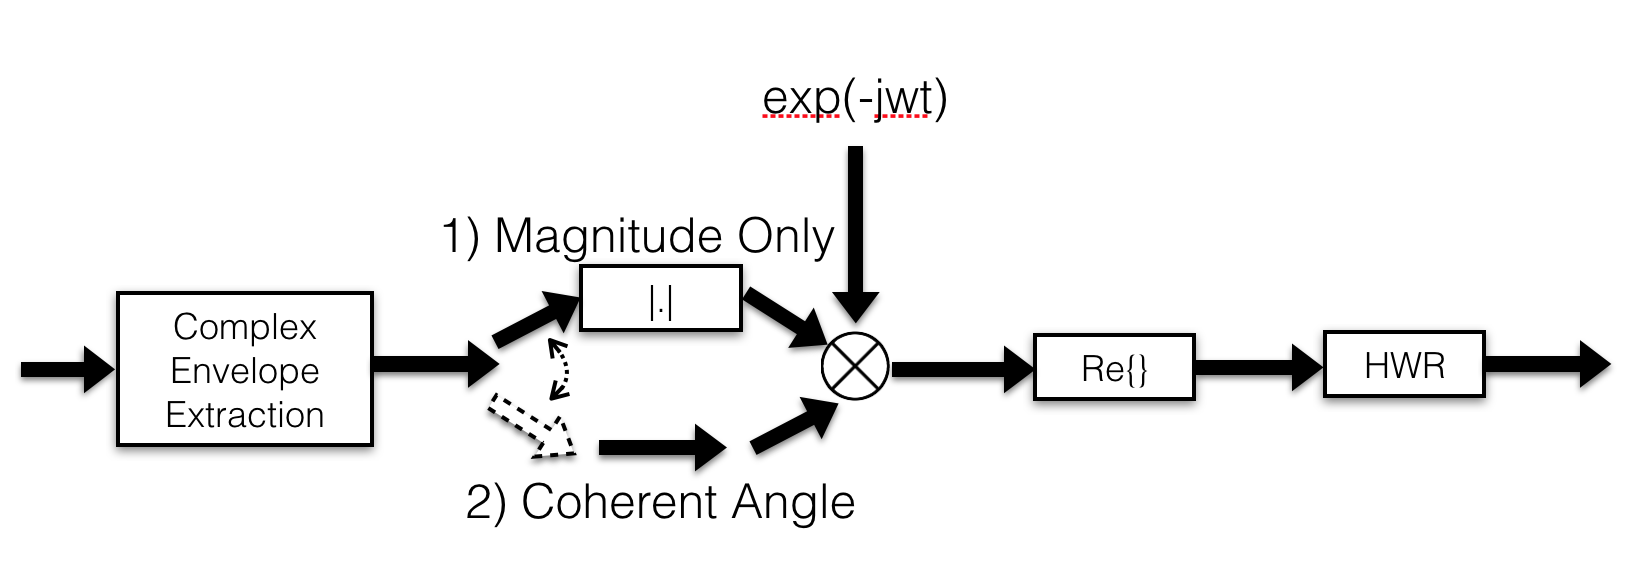
\includegraphics[width=1\textwidth]{coherent_angle}   
    \caption{Magnitude Only VS Coherent Angle Encoding Block Diagrams}
    \label{fig:coherent_angle}
\end{figure}

Let's consider a signal where our $k$th bandpass component represents the $k$th harmonic and is of the form

\begin{align}
x_k[n] =& A_k[n]cos(2\pi kF_0n + \phi_k[n]) \\
BW \leq& F_0 \nonumber
\end{align}

where $A_k[n]$ represents a real nonnegative amplitude.  And $BW$ is the bandpass signal's bandwidth.  We may assume $F_0[n] = F_0$ is constant without loss of generality so long as $F_0[n]$ is roughly constant within each processing frame.

Let's assume our filter is an ideal brick-wall filter.

%TODO should be 2pif / Fs

\begin{align}
h[n] \Longleftrightarrow& H(e^{j2\pi f}) \\
H(e^{j2\pi f}) =& 1, \quad |f| < \frac{F_0}{2} \\
=& 0, \quad else \nonumber
\end{align}

Our coherent harmonic envelopes for each method will be

%TODO
% can't assume this from (3.17) and (3.19)
% maybe derive this? appendix?
\begin{align}
\label{eq:realVSmag1}
m^{(1)}_{k,harmonic}[n] =& A_k[n] \\
m^{(2)}_{k,harmonic}[n] =& A_k[n]e^{j\phi_k[n]}
\end{align}

Let us define $Rect\{y_k[n]\}$ as the half-wave rectified carrier-modulator signal which is our end goal.  Using our first harmonic method

\begin{align}
y_k^{(1)}[n] =& m^{(1)}_{k,harmonic}[n] cos(2\pi F_0 n) \\
=& A_k[n] cos(2\pi F_0 n) \nonumber
\end{align}

Alternatively, with our second method we get

\begin{align}
y_k^2[n] =& Re\{ 2m^{(2)}_{k,harmonic}[n] e^{j2\pi F_0 n} \}  \\
=& Re\{ 2A_k[n]e^{j(2\pi F_0 n + \phi_k[n])} \} \nonumber \\
=& A_k[n]cos(2\pi F_0 n + \phi_k[n]) \nonumber
\end{align}

It is clear that the difference between $y_k^1[n]$ and $y_k^2[n]$ is simply the extra term, $\phi_k[n]$.  What this means may be best shown by example.

In figure \ref{fig:real_vs_magnitude_example} we see that when taking the magnitude, we force symmetry about $0$.  We see that the green much better represents the blue than the red does by preserving the spectral asymmetries that manifest themselves in the angle, not magnitude.  It is unnatural and certainly won't happen in real world scenarios that a subband signal will be symmetric about the downshift frequency, however magnitude only methods force this to be true.

\begin{figure}[!ht]
  \centering
    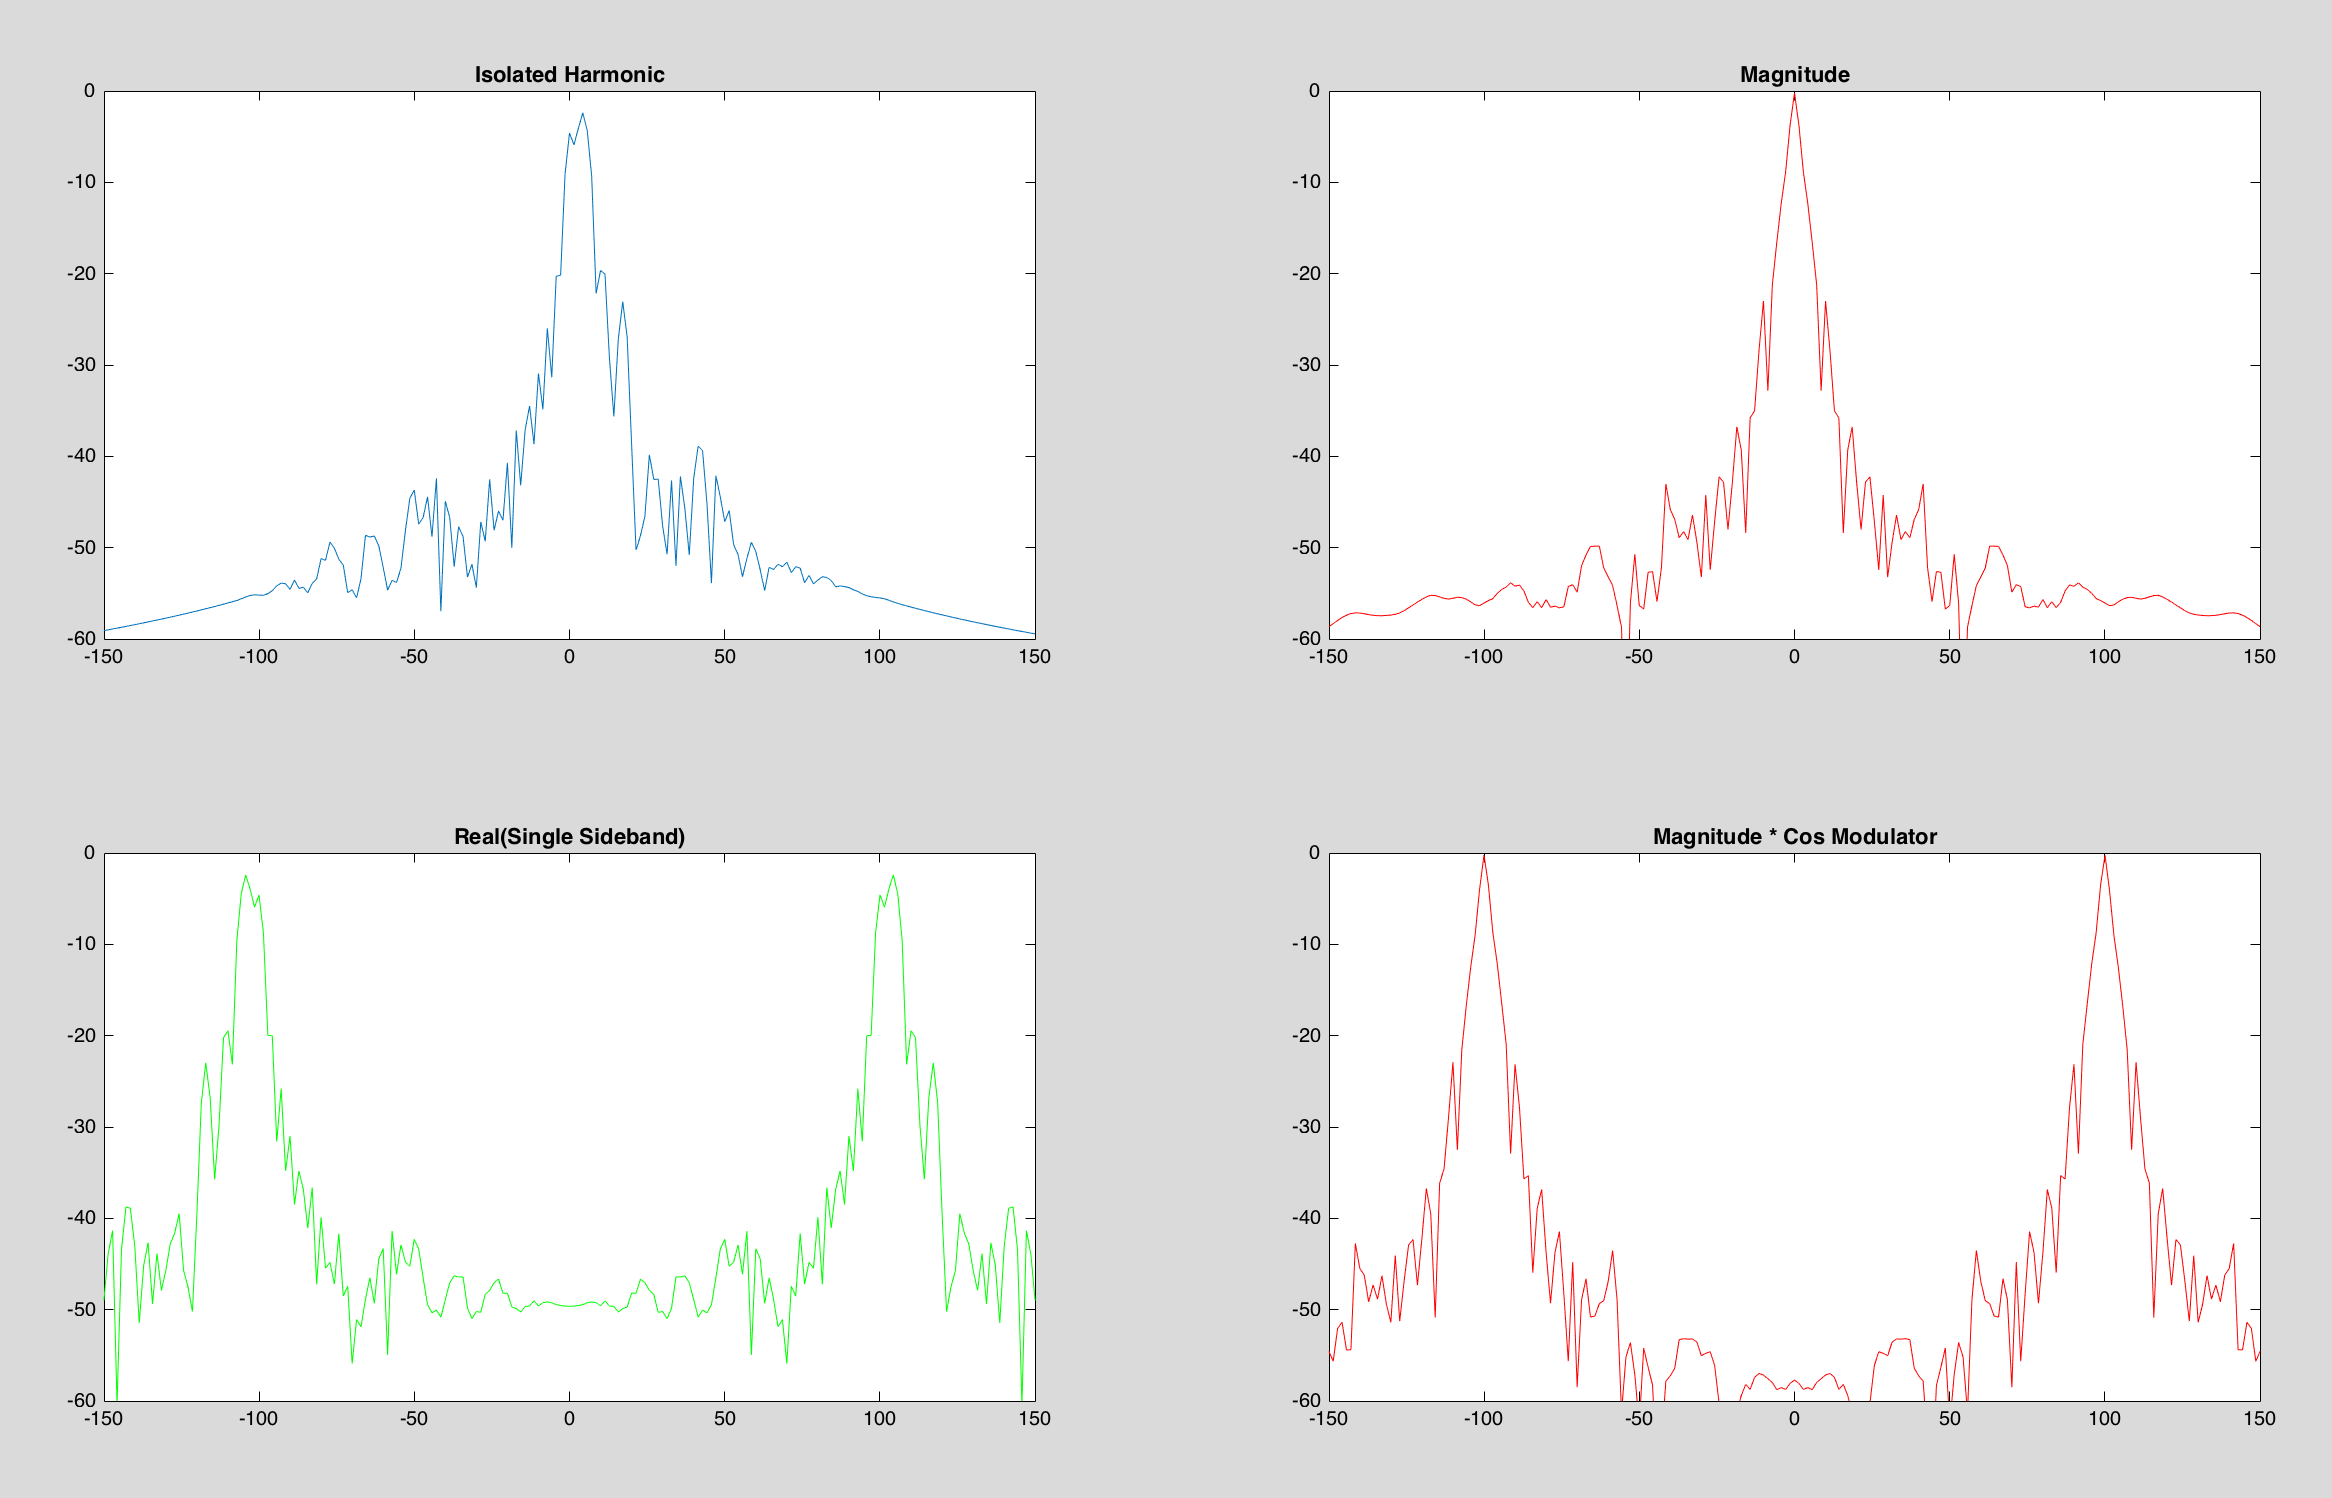
\includegraphics[width=1\textwidth]{real_vs_magnitude_example}   
    \caption{Cello Example}
    \label{fig:real_vs_magnitude_example}
\end{figure}

\subsection{Appropriate Scaling}

Despite better representing the signal, there is still an issue with $y_k^2[n]$.  A more correct method is actually

\begin{align}
\label{eq:realVSmag3}
m^{(3)}_{k,harmonic}[n] =& A_k[n]e^{j\frac{1}{k} unwrap(\phi_k[n])} \\
y_k^3[n] =& Re\{ 2 m^{(3)}_{k,harmonic}[n] e^{j2\pi F_0 n} \}  \\
=& A_k[n]cos\Big(2\pi F_0 n + \frac{1}{k}unwrap(\phi_k[n])\Big) \nonumber
\end{align}


Why do we need the $\frac{1}{k}$ term?  Let's consider an example where our true pitch estimate is actually $F_{0,ground truth} = F_0 + F_{err}$.  So,

\begin{align}
x_k[n] = A_k[n]cos\Big(2\pi k(F_0 + F_{err})n + \phi_k[n]\Big)
\end{align}

In this case

\begin{align}
y_k^{(2)}[n] =& A_k[n]cos\Big(2\pi (F_0 + kF_{err})n + \frac{1}{k}unwrap(\phi_k[n])\Big) \\
y_k^{(3)}[n] =& A_k[n]cos\Big(2\pi (F_0 + F_{err})n + \frac{1}{k}unwrap(\phi_k[n])\Big)
\end{align}

Essentially the term $\phi_k[n]$ may be thought of as the deviation from $kF_0$.  If we downshift the signal such that $kF_0$ is scaled to $F_0$ then it is appropriate that we scale $\phi_k[n]$ similarly.

\subsection{Efficacy}

Let us now consider the efficacy of \ref{eq:realVSmag1} versus  \ref{eq:realVSmag3}.

One hypothesis is that $\phi_k[n]$ may encode the noise-like characteristics of a signal, in which case it would remain constant for a pure sinusoid and fluctuate randomly for noise.  Put to test, the harmonic phase preservation did little to affect the signal and this was confirmed by testing varying filter bandwidths as well.  In comparison of a toy experiment, the choice of filter bandwidth dominated noise-like qualities, with wider bandwidth capturing more of the variations.

Since the term $\phi_k[n]$ does not distinguish noise-like signals from narrowband sinusoidal signals, it is only really preserving phase alignment.  But this begs the question, what does it mean to preserve the phase of a harmonic when downshifted to $F_0$?  It is questionable as to whether this even has any logical meaning.

% It means every k'th peak will be lined up with the downshifted peak, that being said that probably doesn't mean a whole lot in terms of important information
% perhaps show a figure of this?

Furthermore, it has been suggested in [REF F0mod and kaibao??] that phase alignment is important for pitch perception in CIs.  By using a magnitude-only method we guarantee alignment across channels.

%Is an example necessary? Noise vs Saw example...used "shh" vs "saw" test.  at least when listening to the simulations, the processing essentially sounds like narrowband resonant filters.  The noise-like sounds are completely dominated by the filter bandwidth and the phase-information is not noticeable at all.

Having considered this option as not a path worth further investigating, for the rest of this document we will consider envelope and carrier separately with each being a real nonnegative signal at the final output.

\section{The Relationships}

All of our methods are summarized in table~\ref{table:envelope_extraction_methods}.  We will now consider the relationships between each of these.

\begin{table}
\begin{center}
\begin{tabular}{| r | c |}
  \hline
  \textbf{Method} & $m_k[n] = $ \\ \hline
  CIS & $\Big| x[n] * h_k[n] \Big| * h_{lp}[n]$ \\ \hline
  Hilbert & $\Big| \widehat{x}_k[n] \Big| = \Big| x[n] * h_k[n] + j\mathcal{H}\{x[n] * h_k[n]\} \Big|$ \\ \hline
  STFT & $\frac{1}{Nw[0]}  \Big\vert x[n] e^{-j\frac{2\pi}{N}kn} * w[-n] \Big\vert$ \\ \hline
  Harmonic Coherent & $\Big| x[n] e^{-jk\phi_0 [n]} * h\big[n, F_0[n] \big] \Big|, \qquad \phi_0[n] = \frac{2\pi}{F_s} \sum_{p=0}^{n} F_0[p]$ \\ \hline
\end{tabular}
\end{center}
\caption{Envelope Extraction Methods}\label{table:envelope_extraction_methods}
\end{table}

\subsection{Hilbert VS STFT}

Let us start by comparing the Hilbert and STFT methods.  Since "the Hilbert transform of a convolution is the convolution of the Hilbert transform on either factor" [wikipedia] we have 

\begin{align}
\label{eq:x_analytic}
\widehat{x}_k[n] =& x_k[n] + jH\{x_k[n]\} \nonumber \\
=& x[n] * h_k[n] + jH\{x[n] * h_k[n]\} \nonumber \\
=& x[n] * h_k[n] + x[n] * jH\{h_k[n]\} \nonumber \\
=& x[n] * [h_k[n]+  jH\{h_k[n]\}]
\end{align}

Now let us define our filter specifically as

\begin{align}
\label{eq:hilbert_constrained_filter}
h_k[n] = \frac{1}{Nw[0]}w[-n]cos(\frac{2\pi}{N}kn)
\end{align}

If we assume the sidelobes of $w[n]$ roll-off sufficiently fast in relation to the center-frequency $\frac{2\pi k}{N}$, we may approximate

\begin{align}
\mathcal{H}\{h_k[n]\} \approx& \frac{1}{Nw[0]}w[-n] H\{cos(\frac{2\pi}{N}kn)\} \nonumber \\
=& \frac{1}{Nw[0]}w[-n]sin(\frac{2\pi}{N}kn)
\end{align}

%To verify the previous equation, consider the extremes:
%1) $w[n] = 1$
%2) $w[n] = \delta[n]$
%TODO verify this approximation claim

Plugging our filter \ref{eq:hilbert_constrained_filter} into \ref{eq:x_analytic}

\begin{align}
\widehat{x}_k[n] \approx& x[n] * \frac{1}{Nw[0]}w[-n]e^{j\frac{2\pi}{N}kn} \nonumber \\
=& \frac{1}{Nw[0]}\sum\limits_{r=-\infty}^{\infty}x[n - r] w[-r] e^{j\frac{2\pi}{N}kr} \nonumber \\
\textrm{Let} \quad r' = -r \nonumber \\
=& \frac{1}{Nw[0]}\sum\limits_{r'=0}^{N-1} x[n + r'] w[r'] e^{-j\frac{2\pi}{N}kr'} \nonumber \\
=& \frac{1}{Nw[0]}\bigg[e^{-j\frac{2\pi}{N}kn} \sum\limits_{r'=0}^{N-1} x[n + r'] w[r'] e^{-j\frac{2\pi}{N}kr'}\bigg]e^{j\frac{2\pi}{N}kn} \nonumber \\
=& \frac{1}{Nw[0]}X[n,i]e^{j\frac{2\pi}{N}kn} \nonumber \\
=& \Bigg( \frac{1}{Nw[0]}  x[n] e^{-j\frac{2\pi}{N}kn} * w[-n] \Bigg) e^{j\frac{2\pi}{N}kn} \\
\end{align}

When we take the magnitude the complex exponential term goes to 1 and we are left with the STFT envelope.  We come to the conclusion that under the assumption of fast sidelobe rolloff we may define a filter bank of $\frac{N}{2} + 1$ filters

\begin{align}
h_k[n] = w[-n]cos(\frac{2\pi}{N}kn), \qquad 0 \leq k \leq \frac{N}{2}
\end{align}

such that

\begin{align}
m_{k,hilbert}[n] \approx& m_{k,STFT}[n]
\end{align}

What this tells us is that the Hilbert decomposition may be viewed as a superset of the STFT method that is not constrained to uniform bandwidth linearly spaced filters.

\subsection{STFT vs Harmonic}

Let us now consider the relationship between STFT and harmonic coherent.  We may choose our filter to be time-invariant and define it as

\begin{align}
h\big[n, F_0[n] \big] = \frac{1}{Nw[0]} w[-n]
\end{align}

where $w[n]$ is a lowpass filter and 
\begin{align}
w[n] \neq& 0, \qquad 0 \leq n < N \nonumber \\
=& 0, \qquad else
\end{align}

In this case,

\begin{align}
m_{k,harmonic}[n] =& \Big| x[n] e^{-jk\phi_0 [n]} *  \frac{1}{Nw[0]} w[-n] \Big|  \nonumber \\
=& \frac{1}{Nw[0]} \Big| x[n] e^{-jk\phi_0 [n]} *  w[-n] \Big|
\end{align}

This bears striking resemblance to equation \ref{eq:STFT_envelope}.  We can see that in the case that $F_0[n] = \frac{F_s}{N}$,

\begin{align}
m_{k,harmonic}[n] = m_{k,STFT}[n]
\end{align}

More generally, for any window of time $n$ to $n + N - 1$ where $F_0[n]$ is constant

%check appendix code 810982374981u23h for derivation
\begin{align}
m_{k,harmonic}[n] =& \frac{1}{Nw[0]} \Bigg| X\Big[n, \frac{N}{1} \frac{F_0[n]}{F_s} k \Big) \Bigg| \nonumber \\
\label{eq:harmonic-to-stft}
=& \frac{1}{Nw[0]} \Bigg| X\Big[n, \lambda[n]k\Big) \Bigg|
\end{align}

where $\lambda[n] = \frac{N}{1} \frac{F_0[n]}{F_s}$.  The ``$)$'' is to denote that the frequency term is not necessarily an integer.

It is important to note that in practice $\lambda[n]$ is not a continuous variable.  It is constrained by the quantization of the implemented pitch tracker.  Provided this quantization we may compute any term $X[n, \lambda[n]k)$ by, leaving all else the same, zero-padding our FFT.

What this tells us is that in practice, we may approximate $m_{k,harmonic}[n]$ using $F_0[n]$ and a zero-padded STFT under the assumptions:

1) $F_0[n]$ is quantized

2) $F_0[n]$ is roughly constant withing a time window of $\frac{N}{Fs}$ seconds

and the restriction:

3) $h\Big[n, F_0[n] \Big]$ is time-invariant, i.e. $h\Big[n, F_0[n] \Big] = h[n]$

\subsection{CIS VS Hilbert}

Provided our envelope definitions

\begin{align}
m_{k,CIS}[n] =& \Big| x_k[n] \Big| * h_{lp}[n] \nonumber \\
m_{k,Hilbert}[n] =& \Big| \widehat{x}_k[n] \Big| \nonumber
\end{align}

We define an ideal brick-wall filter as

\begin{align}
H_k(f) =& \mathcal{F}\Big\{ h_k[n]  \Big\} \\
H_k(f) =& 1, \quad f_k - \frac{1}{2} f_{bw} < |f| < f_k + \frac{1}{2} f_{bw} \\
=& 0, \quad \mathrm{else}
\end{align}

\begin{align}
X(f) =& \mathcal{F}\Big\{ x[n] \Big\} \\
X_{k}(f) =& \mathcal{F}\Big\{ x_k[n] \Big\} \\
\widehat{X}_{k}(f) =& \mathcal{F}\Big\{ \widehat{x}_k[n]  \Big\}
\end{align}

\begin{align}
X_{k}(f) =& X(f), \quad f_k - \frac{1}{2} f_{bw} < |f| < f_k + \frac{1}{2} f_{bw} \\
=& 0, \quad \mathrm{else} \\
\widehat{X}_{k}(f) =& X(f), \quad f_k - \frac{1}{2} f_{bw} < f < f_k + \frac{1}{2} f_{bw} \\
=& 0, \quad \mathrm{else}
\end{align}

\begin{align}
Y_{k}^1(f) =& \mathcal{F}\Big\{ \Big| \widehat{x}_k[n] \Big|^2  \Big\} \\
Y_{k}^2(f) =& \mathcal{F}\Big\{ \Big| x_k[n] \Big|^2  \Big\}
\end{align}

\begin{align}
Y_{k}^1(f) =& \widehat{X}_{k}(f) * \widehat{X}_{k}^*(-f) \\
=& \int\limits_{-\infty}^{\infty} \widehat{X}_{k}(f - r) \widehat{X}_{k}^*(-r)dr \\
=& \int\limits_{-\infty}^{\infty} \widehat{X}_{k}(r + f) \widehat{X}_{k}^*(r)dr
\end{align}

We can narrow the integration bounds provided the restrictions

\begin{align}
\widehat{X}_{k}^*(r) \neq& 0 \Rightarrow  f_k - \frac{1}{2} f_{bw} < r < f_k + \frac{1}{2} f_{bw} \\
\widehat{X}_{k}(r + f) \neq& 0 \Rightarrow  f_k - \frac{1}{2} f_{bw} - f < r < f_k + \frac{1}{2} f_{bw} - f \\
a =& max\Big( f_k - \frac{1}{2} f_{bw},  f_k - \frac{1}{2} f_{bw} - f\Big) \\
b =& min\Big( f_k + \frac{1}{2} f_{bw},  f_k + \frac{1}{2} f_{bw} - f\Big) \\
Y_{k}^1(f) =& \int\limits_{a}^{b} \widehat{X}_{k}(r + f) \widehat{X}_{k}^*(r)dr, \quad -f_{bw} < f < f_{bw} \\
=& 0, \quad \mathrm{else}
\end{align}

For $Y_k^2(f)$ there are actually three non-zero bands.

\begin{align}
Y_{k}^2(f) =& X_{k}(f) * X_{k}^*(-f) \\
=& \int\limits_{-\infty}^{\infty} X_{k}(r + f) X_{k}^*(r)dr
\end{align}

Case 1: $-2f_k - f_{bw} < f < -2f_k + f_{bw}$

\begin{align}
Y_{k}^2(f) =& \int\limits_{a}^{b} X_{k}(r + f) X_{k}^*(r)dr \\
a =& max\Big( f_k - \frac{1}{2} f_{bw},  f_k - \frac{1}{2} f_{bw} - f\Big) \\
b =& min\Big( f_k + \frac{1}{2} f_{bw},  f_k + \frac{1}{2} f_{bw} - f\Big)
\end{align}

Case 2: $2f_k - f_{bw} < f < 2f_k + f_{bw}$

\begin{align}
Y_{k}^2(f) =& \int\limits_{a}^{b} X_{k}(r + f) X_{k}^*(r)dr \\
a =& max\Big( -f_k - \frac{1}{2} f_{bw},  -f_k - \frac{1}{2} f_{bw} - f\Big) \\
b =& min\Big( -f_k + \frac{1}{2} f_{bw},  -f_k + \frac{1}{2} f_{bw} - f\Big)
\end{align}

Case 3: $- f_{bw} < f < f_{bw}$

This case is unique because there are two points of intersection.  We can break up the integral into a sum.  The first integral is exactly the same as in $Y^1_k(f)$.

\begin{align}
Y_{k}^2(f) =& \int\limits_{a_1}^{b_1} X_{k}(r + f) X_{k}^*(r)dr + \int\limits_{a_2}^{b_2} X_{k}(r + f) X_{k}^*(r)dr \\
a_1 =& max\Big( f_k - \frac{1}{2} f_{bw},  f_k - \frac{1}{2} f_{bw} - f\Big) \\
b_1 =& min\Big( f_k + \frac{1}{2} f_{bw},  f_k + \frac{1}{2} f_{bw} - f\Big) \\
a_2 =& max\Big( -f_k - \frac{1}{2} f_{bw},  -f_k - \frac{1}{2} f_{bw} - f\Big) \\
b_2 =& min\Big( -f_k + \frac{1}{2} f_{bw},  -f_k + \frac{1}{2} f_{bw} - f\Big)
\end{align}

Using the Hermitian symmetry of the real-valued $x[n]$,

\begin{align}
Y_{k}^2(f) =& \int\limits_{a_1}^{b_1} X_{k}(r + f) X_{k}^*(r)dr + \int\limits_{a_2}^{b_2} X_{k}^*(-r - f) X_{k}(-r)dr \\
r' = -r - f \nonumber \\
Y_{k}^2(f) =& \int\limits_{a_1}^{b_1} X_{k}(r + f) X_{k}^*(r)dr + \int\limits_{a_1}^{b_1} X_{k}^*(r') X_{k}(r' + f)dr' \\
=& 2 \int\limits_{a_1}^{b_1} X_{k}(r + f) X_{k}^*(r)dr \\
=& 2 Y_k^1(f)
\end{align}

If we lowpass filter $Y_k^2(f)$ with a filter defined

\begin{align}
H_{lp}(f) =& \frac{1}{2}, \quad |f| < f_{bw} \\
=& 0, \quad 2f_k - f_{bw} < |f| < 2f_k + f_{bw}
\end{align}

then

\begin{align}
Y_{k}^2(f) =& Y_k^1(f) \quad \forall f
\end{align}

We conclude that 

\begin{align}
\label{eq:squared_cis_hilbert}
\Big| x_k[n] \Big|^2 * h_{lp}[n] \approx \Big| \widehat{x}_k[n] \Big|^2
\end{align}

Things to consider are delay and non-deal filters, however provided the distance between baseband and the $\pm2f_k$ terms a sufficient filter is practical in practice.

Now the relationship between $m_{k,CIS}[n]$ and $m_{k,Hilbert}[n]$ is muddled by the nonlinear square root operation, however the nonlinearities induced won't be noticeably distorted by $h_{lp}[n]$.  In practice, there only noticeable difference will be the added delay from the final lowpass filter in the CIS method.

\subsection{Abstract Interpretation}

One of the easier ways to interpret these methods is through a frequency domain analysis.  Figure~\ref{fig:all_the_same} shows an abstract view of the methods.  The input is a magnitude spectrum of a signal with two harmonics. For mathematical convenience the output is actually the squared envelope.  At each step a new operation is applied.  This abstract analysis ignores scale factors that can always be modified by scaling filter coefficients.

\begin{figure}[!ht]
  \centering
    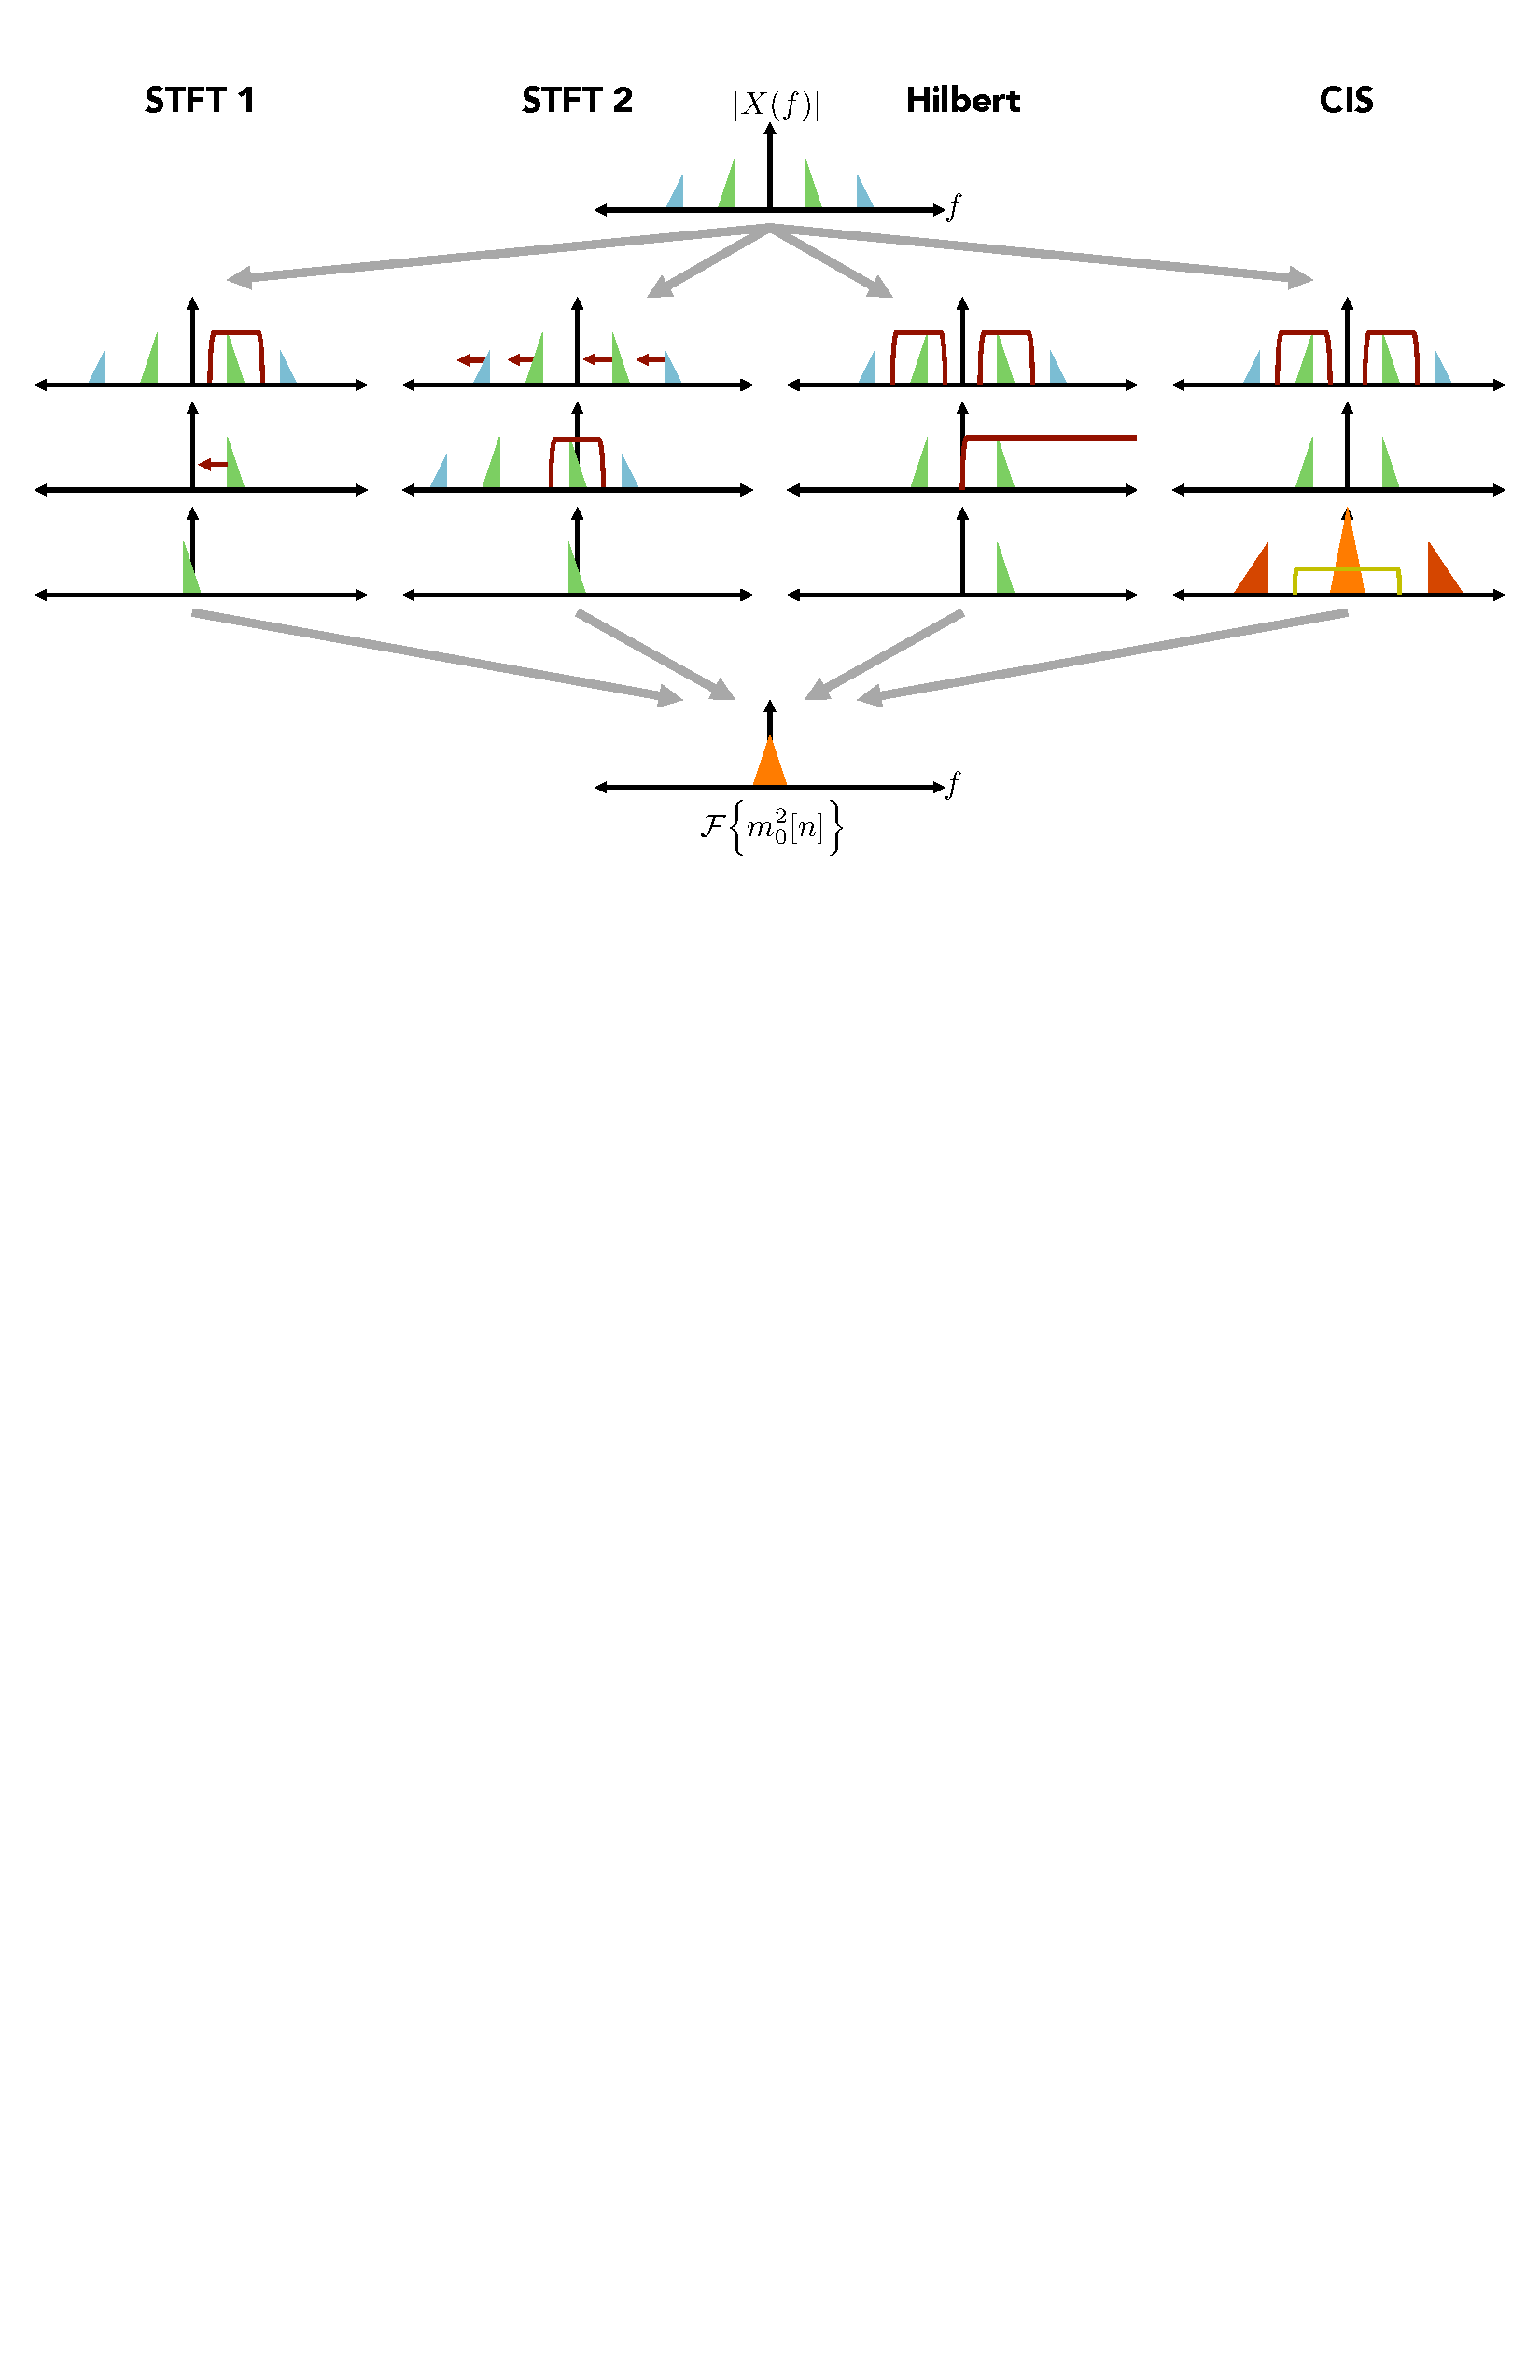
\includegraphics[width=1.0\textwidth]{STFTvsHILBERTvsCIS}   
    \caption{Method Comparison: magnitude spectrum at each step}\label{fig:all_the_same}
\end{figure}

First note that there are two paths for STFT.  This is because there is an ambiguity in the order of operations.  This can be seen mathematically in \ref{eq:stft_2_intepretations}.

\begin{align}
\label{eq:stft_2_intepretations}
e^{-j\frac{2\pi}{N}kn} \Bigg( x[n] * \Big( w[-n]e^{j\frac{2\pi}{N}kn} \Big) \Bigg) = \Big( x[n] e^{-j\frac{2\pi}{N}kn} \Big) * w[-n]
\end{align}

The left side of \ref{eq:stft_2_intepretations} corresponds to the STFT 1 path.  First an analytic bandpass filter centered at radian frequency $\frac{2\pi k}{N}$ is applied.  The output of that is then downshifted to baseband.

The right side of \ref{eq:stft_2_intepretations} corresponds to the STFT 2 path.  We first downshift by radian frequency $\frac{2\pi k}{N}$, then lowpass filter.

For both STFT 1 and STFT 2 the final operation is a magnitude.

The harmonic coherent method is missing from figure~\ref{fig:all_the_same}.  This is because ignoring exact details of downshift frequency and filter coefficients, it is actually the same as the STFT method: downshift followed by lowpass filter.

Let's move on the the Hilbert envelope.  In figure~\ref{fig:all_the_same} we first bandpass filter, then acquire the analytic signal, which is equivalent to setting the negative frequencies to zero.  The final operation is to take the magnitude squared, which is invariant to frequency shifts.  From this abstract view, we should expect the same result as the STFT method.

In CIS, we see that taking the magnitude squared of the real bandpass signal causes double frequency terms, and the baseband term is scaled by a factor of 2.  The final filter operation rescales the baseband term and eliminates the double frequency terms.

\section{Summary}

So what are the differences?  To come to the conclusions made, some assumptions had to be made.  We found that the Hilbert and CIS methods are approximately the same.  STFT decomposition is a subset of the Hilbert method where the filterbank is comprised of uniform-bandwidth linearly spaced filters.  Coherent harmonic is a expansion of STFT decomposition using the fundamental frequency of a signal to adaptively change downshift frequency and filter bandwidth.

In \ref{eq:envelope_extraction_general} we generalize the considered methods.  $h_k\Big[n,F_0[n]\Big]$ is a function of $k$ allowing for non-uniform bandwidths and a function of $F_0[n]$, allowing for coherent filter adaptation.  Similarly, $\omega_k\big[F_0[n]\big]$ is a function of $F_0[n]$, allowing for coherent downshift frequencies.

\begin{align}
\label{eq:envelope_extraction_general}
m_k[n] =& \Big| x[n]e^{-j \omega_k\big[F_0[n]\big]n} * h_k\big[n,F_0[n]\big]  \Big|
%m_k[n] =& \Big| \widehat{x}[n]e^{-j \omega_k[x]n} * h_k[n,x]  \Big|
\end{align}

In the next chapter we will investigate encoding harmonics in cochlear implants using our generalized envelope extraction equation.

% ========== Chapter 4

\chapter{Harmonic Envelope Extraction}\label{ch:harmonic_envelopes}

We want to come up with an envelope extraction system that best represents harmonic signals.  Since harmonic signals have a specific structure, we model our harmonic signal as a restricted sum-of-products model.  We can define our carriers from equation~\ref{eq:sum_of_products} as centered at multiples of $F_0$. In this representation $x_0[n]$ is the fundamental centered at $F_0$, $x_1[n]$ is the 1st harmonic centered at $2F_0$, etc.  Without loss of generality, we will consider the analytic signal, $\widehat{x}[n]$.

\begin{align}
\theta_k[n] =& 2\pi(k+1)\frac{F_0[n]}{F_s}n + \phi_k[n] \\
%\theta_k[n] =& \sum_{p=0}^{n} 2\pi(k+1)\frac{F_0[p]}{F_s} + \phi_k[p] \\
x[n] =& \sum\limits_{k=0}^K m_k[n] cos(\theta_k[n]) \\
\widehat{x}[n] =& \sum\limits_{k=0}^K m_k[n] e^{j\theta_k[n]}
\end{align}

We change our notation slightly from chapter~\ref{ch:envelope_extraction_chapter}.  In this chapter $m_k[n]$ is the unknown desired envelope, and $\tilde{m}_k[n]$ is our extracted envelope estimate.

\begin{align}
\label{eq:envelope_extraction}
\tilde{m}_k[n] =& \Big| x[n]e^{-j \omega_k\big[F_0[n]\big]n} * h_k\big[n,F_0[n]\big]  \Big|
%\tilde{m}_k[n] =& \Big| \widehat{x}[n]e^{-j \omega_k[x]n} * h_k[n,x]  \Big|
\end{align}

Provided our envelope extraction equation, \ref{eq:envelope_extraction}, our goal is to best represent the desired $m_k[n]$.

The design can be summarized by two things:

\begin{itemize}
\item downshift frequency, $\omega_k\big[F_0[n]\big]$
\item lowpass filter, $h_k\big[n,F_0[n]\big]$
\end{itemize}

If $w_k[\cdot]$ and $h_k[\cdot]$ are functions of $\widehat{x}[n]$ we have coherent envelope extraction.  If they are time-invariant, we have incoherent extraction.

\section{Steady-State Analysis}

We start with the simplest scenario, where $\widehat{x}[n]$ is a steady-state signal.  The conditions we require for this are:

\begin{itemize}
\item constant pitch: $F_0[n] = F_0$
\item narrowband modulator: $m_k[n] \approx constant$ over short periods of time
\item constant phase term: $\phi_k[n] = \phi_k$, we choose $\phi_k[n] = 0$ for cleaner equations however this is not necessary
\end{itemize}

\subsection{3 Harmonic Example: Desired Envelope}

We visualize the frequency domain for a signal with three harmonics ($K = 2$) in figure~\ref{fig:harmonic_envelope}.  For this example we consider the 1st harmonic ($k = 1$), centered at $2F_0$.

Figure~\ref{fig:harmonic_envelope}$(d)$ is the spectrum of the squared envelope, $| \mathcal{F} \{m_1^2[n] \}|$.  We see this relationship in equation~\ref{eq:harmonic_envelope_spectrum_d}

\begin{align}
\label{eq:harmonic_envelope_spectrum_a}
(a)& \quad \widehat{x}[n] \Longleftrightarrow \widehat{X}[n,f)  \\
(b)& \quad \widehat{x}_1[n] \Longleftrightarrow \widehat{X}_1[n,f) \\
(c)& \quad \widehat{x}_1^*[n] \Longleftrightarrow \widehat{X}_1^*[n,-f) \\
\label{eq:harmonic_envelope_spectrum_d}
(d)& \quad m_1^2[n] = \widehat{x}_1[n] \widehat{x}_1^*[n] \Longleftrightarrow \widehat{X}_1[n,f) * \widehat{X}_1^*[n,-f)
\end{align}

\begin{figure}[!ht]
  \centering
    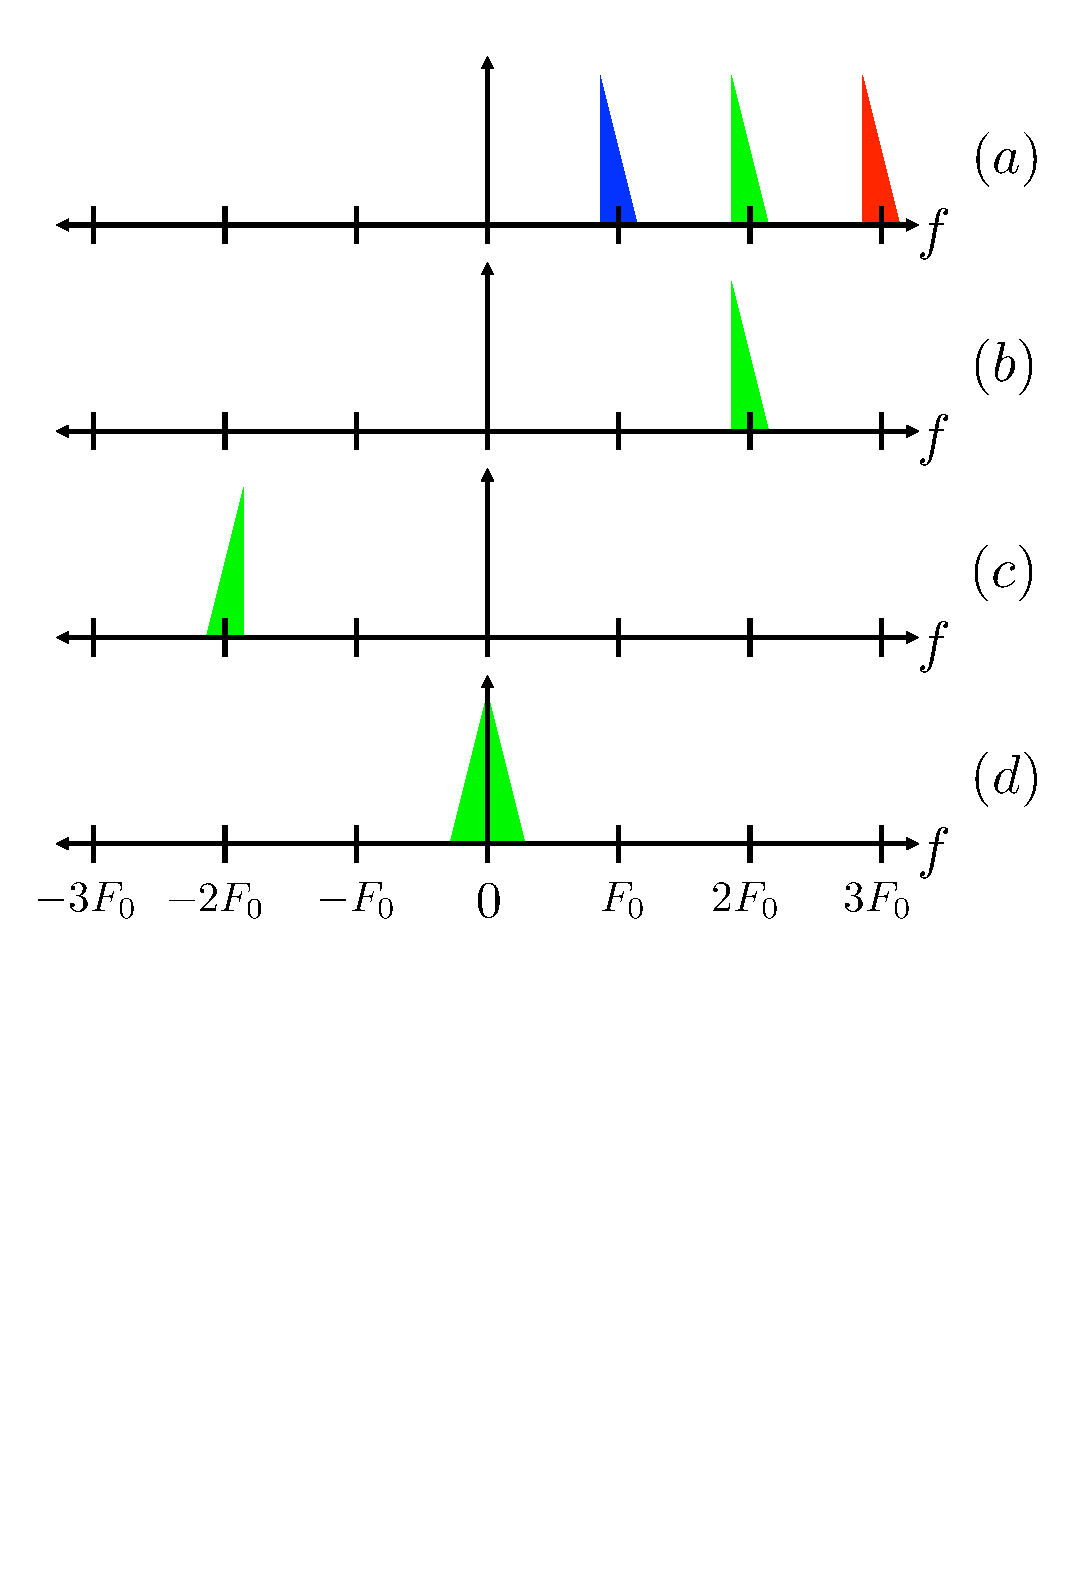
\includegraphics[width=.62\textwidth]{harmonic_envelope}
        \caption{Magnitude of spectrum for equations \ref{eq:harmonic_envelope_spectrum_a} - \ref{eq:harmonic_envelope_spectrum_d}}\label{fig:harmonic_envelope}
%        \caption{$(a) | \widehat{X}[n,f) |$
%    				$(b) | \widehat{X}_1[n,f) |$
%				$(c) | \widehat{X}_1^*[n,-f) |$
%				$(d) | \widehat{X}_1[n,f) * \widehat{X}_1^*[n,-f) |$}
\end{figure}

The envelope can always be acquired from the squared envelope by a final square root operation.  This operation introduces nonlinearities at multiples of $F_0$ that are difficult to analyze.  For mathematical convenience, during our analysis we can consider the squared envelope.  This final square root operation will remain constant across all examples which allows us to not consider it.

\begin{align}
\label{eq:square_root_relationship}
m_1[n] = \Big|\widehat{x}_1[n]\Big| = \Big[ \widehat{x}_1[n] \widehat{x}_1^*[n] \Big]^\frac{1}{2}
\end{align}

\subsection{Estimated Envelope}

Let's now evaluate our estimate, using equation~\ref{eq:envelope_extraction}.  As stated above, we consider the squared envelope.

\begin{align}
\tilde{m}_k^2[n] =& \Big| \widehat{x}[n]e^{-j \omega_kn} * h_k[n]]  \Big|^2 \nonumber \\
%
=& \Bigg|  \sum\limits_{l=0}^K m_l[n]e^{j(\theta_l[n] - \omega_k[n])}*h_k[n] \Bigg|^2 \nonumber \\
%
\approx& \Bigg|  \sum\limits_{l=0}^K m_l[n] \Big(e^{j(\theta_l[n] - \omega_k[n])}*h_k[n] \Big) \Bigg|^2 \nonumber \\
%
\label{eq:estimated_envelope_squared}
=& \Bigg|  \sum\limits_{l=0}^K m_l[n] e^{j\omega_{k,l}n} H_k\big(e^{j\omega_{k,l}}\big) \Bigg|^2 \\
%
\label{eq:downshift_radian_frequency}
\omega_{k,l} =& 2\pi\frac{(l+1)F_0 - F_{ds,k}}{F_s} \\
%
h_k[n] \Longleftrightarrow& H_k\big(e^{j\omega}\big)
\end{align}

$\omega_{k,l}$ is the downshifted center frequency of the $l$'th harmonic for the estimate of the $k$'th envelope.  $H_k\big(e^{j\omega}\big)$ is the discrete Fourier transform (DFT) of $h_k[n]$.

Expanding equation~\ref{eq:estimated_envelope_squared} we get:

\begin{align}
\tilde{m}_k^2[n] =& \sum\limits_{l=0}^K \sum\limits_{i=0}^K m_l[n] m_i^*[n] e^{j(l-i)F_0} H_k\big(e^{j\omega_{k,l}}\big)H_k^*\big(e^{j\omega_{k,i}}\big) \\
%
%
%
=& \sum\limits_{l=0}^K \Big|m_l[n]\Big|^2 \Big|H_k\big(e^{j\omega_{k,l}}\big)\Big|^2 \nonumber \\
%
%
+& e^{-j2\pi \frac{F_0}{Fs}n} \sum\limits_{l=0}^{K-1} m_l[n] m_{l+1}^*[n] H_k\big(e^{j\omega_{k,l}}\big)H_k^*\big(e^{j\omega_{k,l+1}}\big) \nonumber \\
%
+&  e^{j2\pi \frac{F_0}{Fs}n} \sum\limits_{l=1}^{K} m_l[n] m_{l-1}^*[n] H_k\big(e^{j\omega_{k,l}}\big)H_k^*\big(e^{j\omega_{k,l-1}}\big) \nonumber \\
%
%
+& e^{-j2\pi \frac{2F_0}{Fs}n} \sum\limits_{l=0}^{K-2} m_l[n] m_{l+2}^*[n] H_k\big(e^{j\omega_{k,l}}\big)H_k^*\big(e^{j\omega_{k,l+2}}\big) \nonumber \\
%
+& e^{j2\pi \frac{2F_0}{Fs}n}  \sum\limits_{l=2}^{K} m_l[n] m_{l-2}^*[n] H_k\big(e^{j\omega_{k,l}}\big)H_k^*\big(e^{j\omega_{k,l-2}}\big) \nonumber \\
%
%
+& ... \nonumber \\
%
%
+& e^{-j2\pi \frac{KF_0}{Fs}n} m_0[n] m_K^*[n] H_k\big(e^{j\omega_{k,0}}\big)H_k^*\big(e^{j\omega_{k,K}}\big) \nonumber \\
%
+& e^{j2\pi \frac{KF_0}{Fs}n}  m_K[n] m_0^*[n] H_k\big(e^{j\omega_{k,K}}\big)H_k^*\big(e^{j\omega_{k,0}}\big)
\end{align}

We can now think of $\tilde{m}_k[n]$ as a combination of terms each centered at $iF_0$ where the magnitude of each term is:

\begin{align}
\Big| \tilde{m}_{k,iF_0}[n] \Big| =& \Bigg[ \sum\limits_{l=0}^{K-|i|} \Big| m_l[n]\Big| \Big|m_{l+i}[n]\Big| \Big|H_k\big(e^{j\omega_{k,i}}\big)\Big| \Big|H_k\big(e^{j\omega_{k,l+i}}\big)\Big|\Bigg]^\frac{1}{2}, \quad -K \leq i \leq K
\end{align}

Evaluated at DC:

\begin{align}
\Big| \tilde{m}_{k,0F_0}[n] \Big| =& \Bigg[  \sum\limits_{l=0}^K \Big|m_l[n]\Big|^2 \Big|H_k\big(e^{j\omega_{k,l}}\big)\Big|^2 \Bigg]^\frac{1}{2}
\end{align}

\subsection{3 Harmonic Example: Estimated Envelope}

Let's go back to our three harmonic example.  We are again trying to acquire the 1st harmonic, $m_1[n]$ (green).  We define $\omega_1 = 2F_0$.

\begin{figure}[!ht]
  \centering
    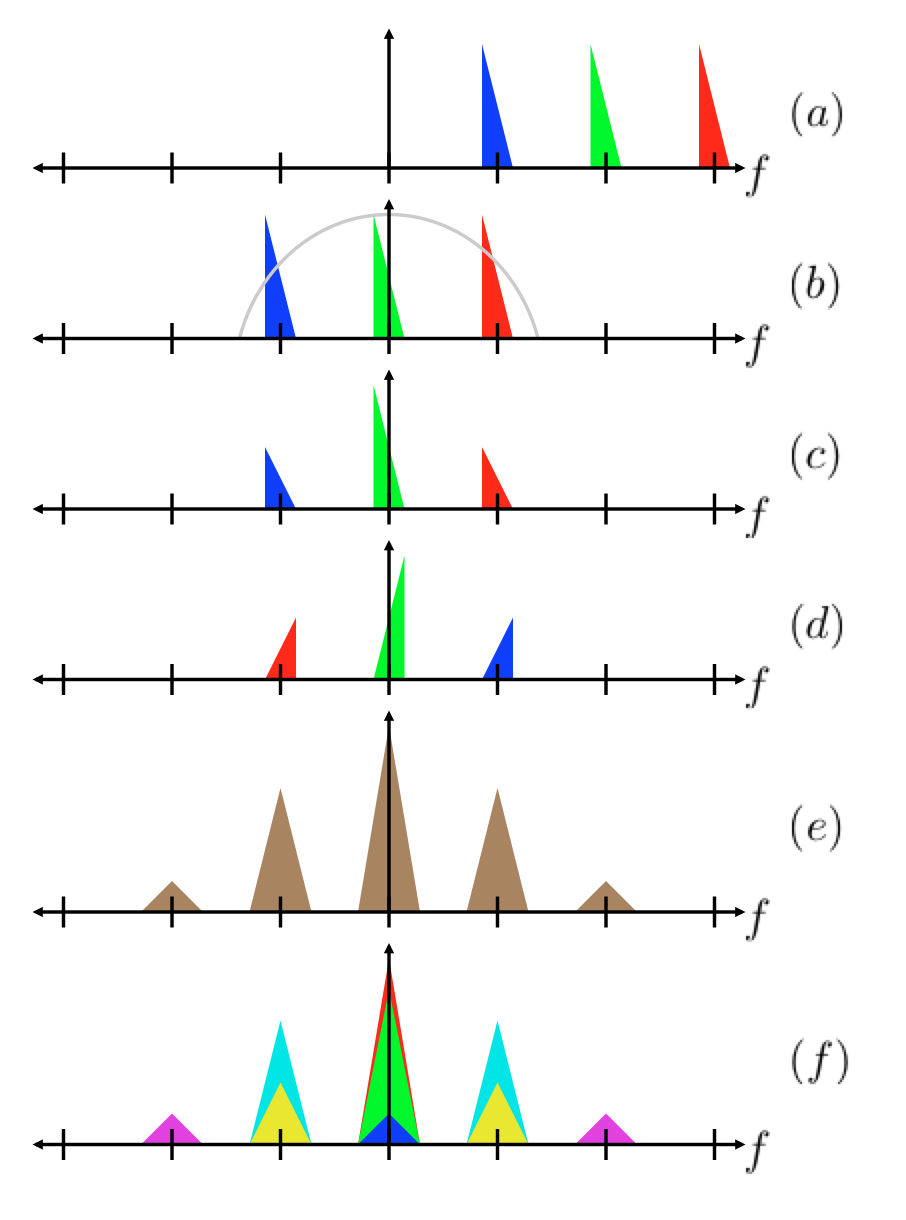
\includegraphics[width=.62\textwidth]{harmonic_envelope_estimate} 
    \caption{$(a) | \widehat{X}[n,f) |$   
    				$(b) | \widehat{X}[n,f - 2F_0) |$  
				$(c) | \widehat{X}[n,f - 2F_0) | | H_1(f) |$
				$(d) | \widehat{X}^*[n,-f + 2F_0) | | H_1(-f) |$
				$(e) | \mathcal{F} \{ \tilde{m}_1^2[n] \} |$
				$(f)$ contributions of separate components of $(e)$}\label{fig:harmonic_envelope_estimate}
\end{figure}

We can see the relationships

\begin{align}
\label{eq:harmonic_estimate_fig_a}
\widehat{x}[n] \Longleftrightarrow& \widehat{X}[n,f) \\
\widehat{x}[n]e^{-j2\pi \frac{2F_0}{F_s}n} \Longleftrightarrow& \widehat{X}[n,f - 2F_0) \\
\widehat{x}[n]e^{-j2\pi \frac{2F_0}{F_s}n} * h_2[n] \Longleftrightarrow& \widehat{X}[n,f - 2F_0) H_1(f) \\
\label{eq:harmonic_estimate_fig_e}
\tilde{m}_1^2[n] \Longleftrightarrow& \widehat{X}[n,f - 2F_0) H_1(f) * \widehat{X}^*[n,-f + 2F_0) H_1^*(-f)
\end{align}

Equations \ref{eq:harmonic_estimate_fig_a}  -\ref{eq:harmonic_estimate_fig_e} are visualized in figure~\ref{fig:harmonic_envelope_estimate}. The interesting part of figure~\ref{fig:harmonic_envelope_estimate} is $(f)$.  We see our green component that we were looking for, however there are a whole lot of other things that we didn't want.

Figure~\ref{fig:harmonic_envelope}$(d)$ is equivalent to the green component of  figure~\ref{fig:harmonic_envelope_estimate}$(f)$ if our filter $|H_1(f)| = 1$ when $f \approx 0$.

The other components come from interactions with the unwanted harmonics that we failed to completely filter out.  For clarity the convolution is visualized in figures \ref{fig:harmonic_envelope_2F0}, \ref{fig:harmonic_envelope_F0}, \ref{fig:harmonic_envelope_0}.  Positive and negative components are mirror images so the positive components are not explicitly visualized.

\begin{figure}[!ht]
   \centering
    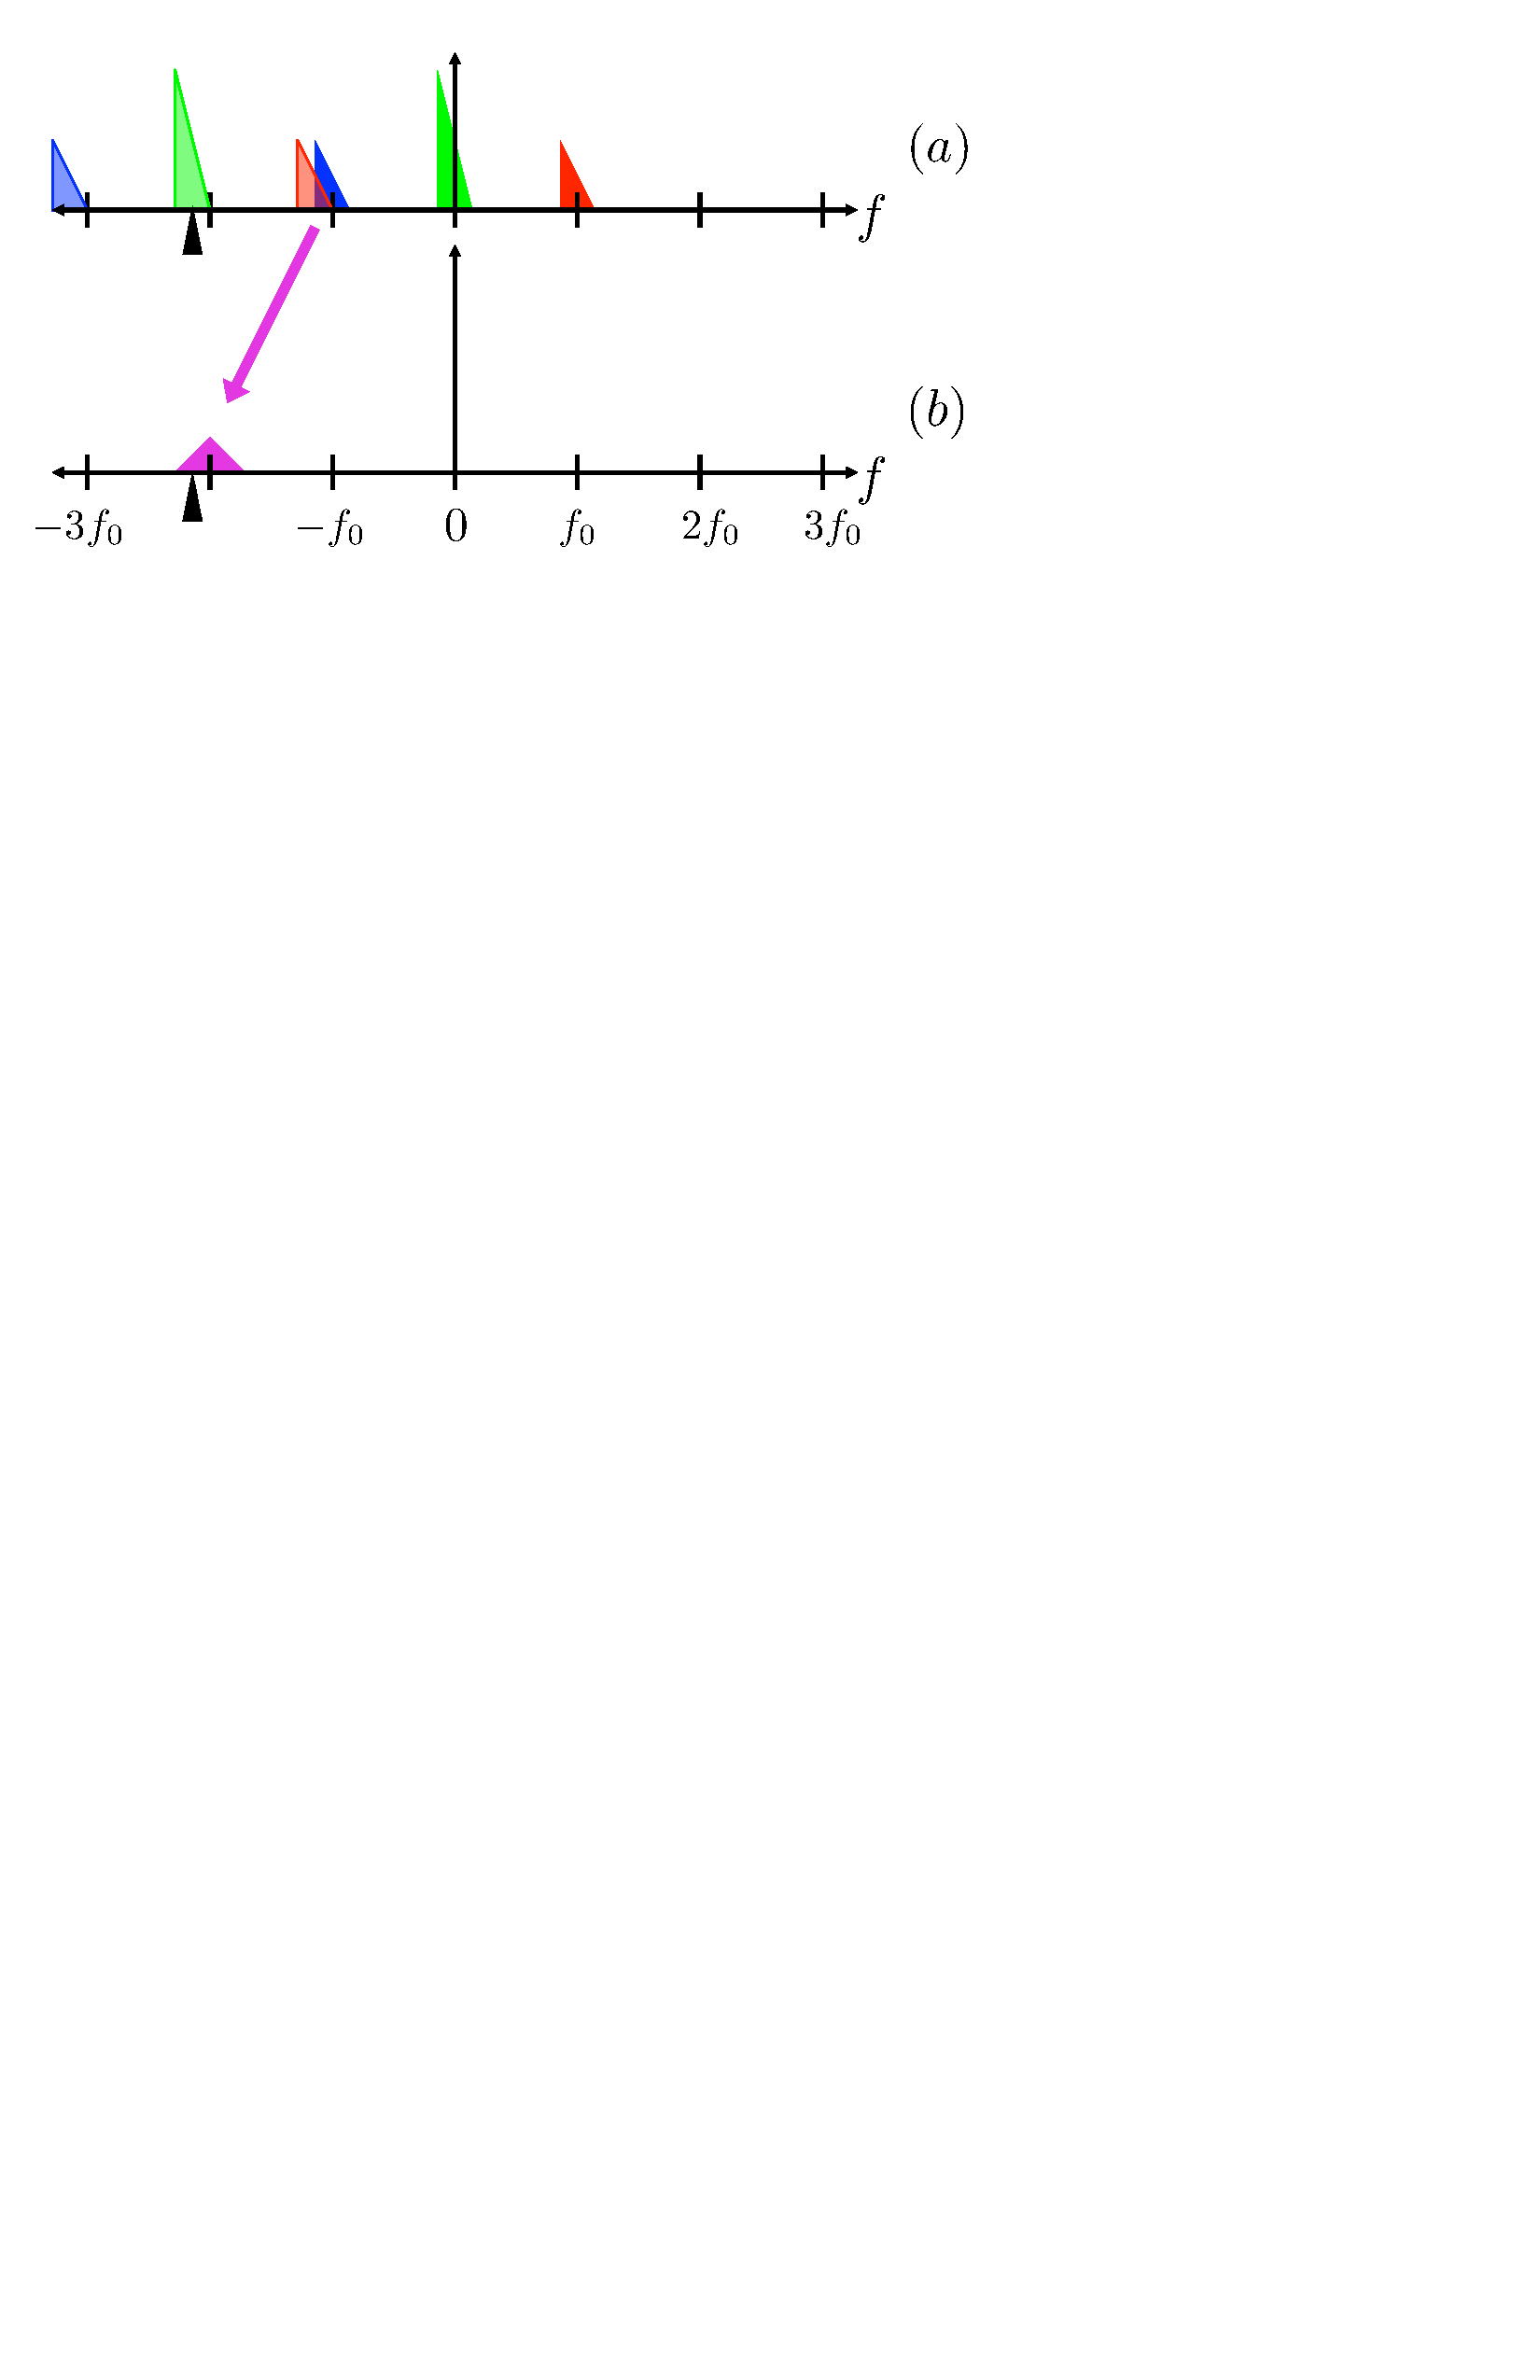
\includegraphics[width=.62\textwidth]{harmonic_envelope_2F0}   
    \caption{Envelope Estimate $-2F_0$ Component}\label{fig:harmonic_envelope_2F0}
    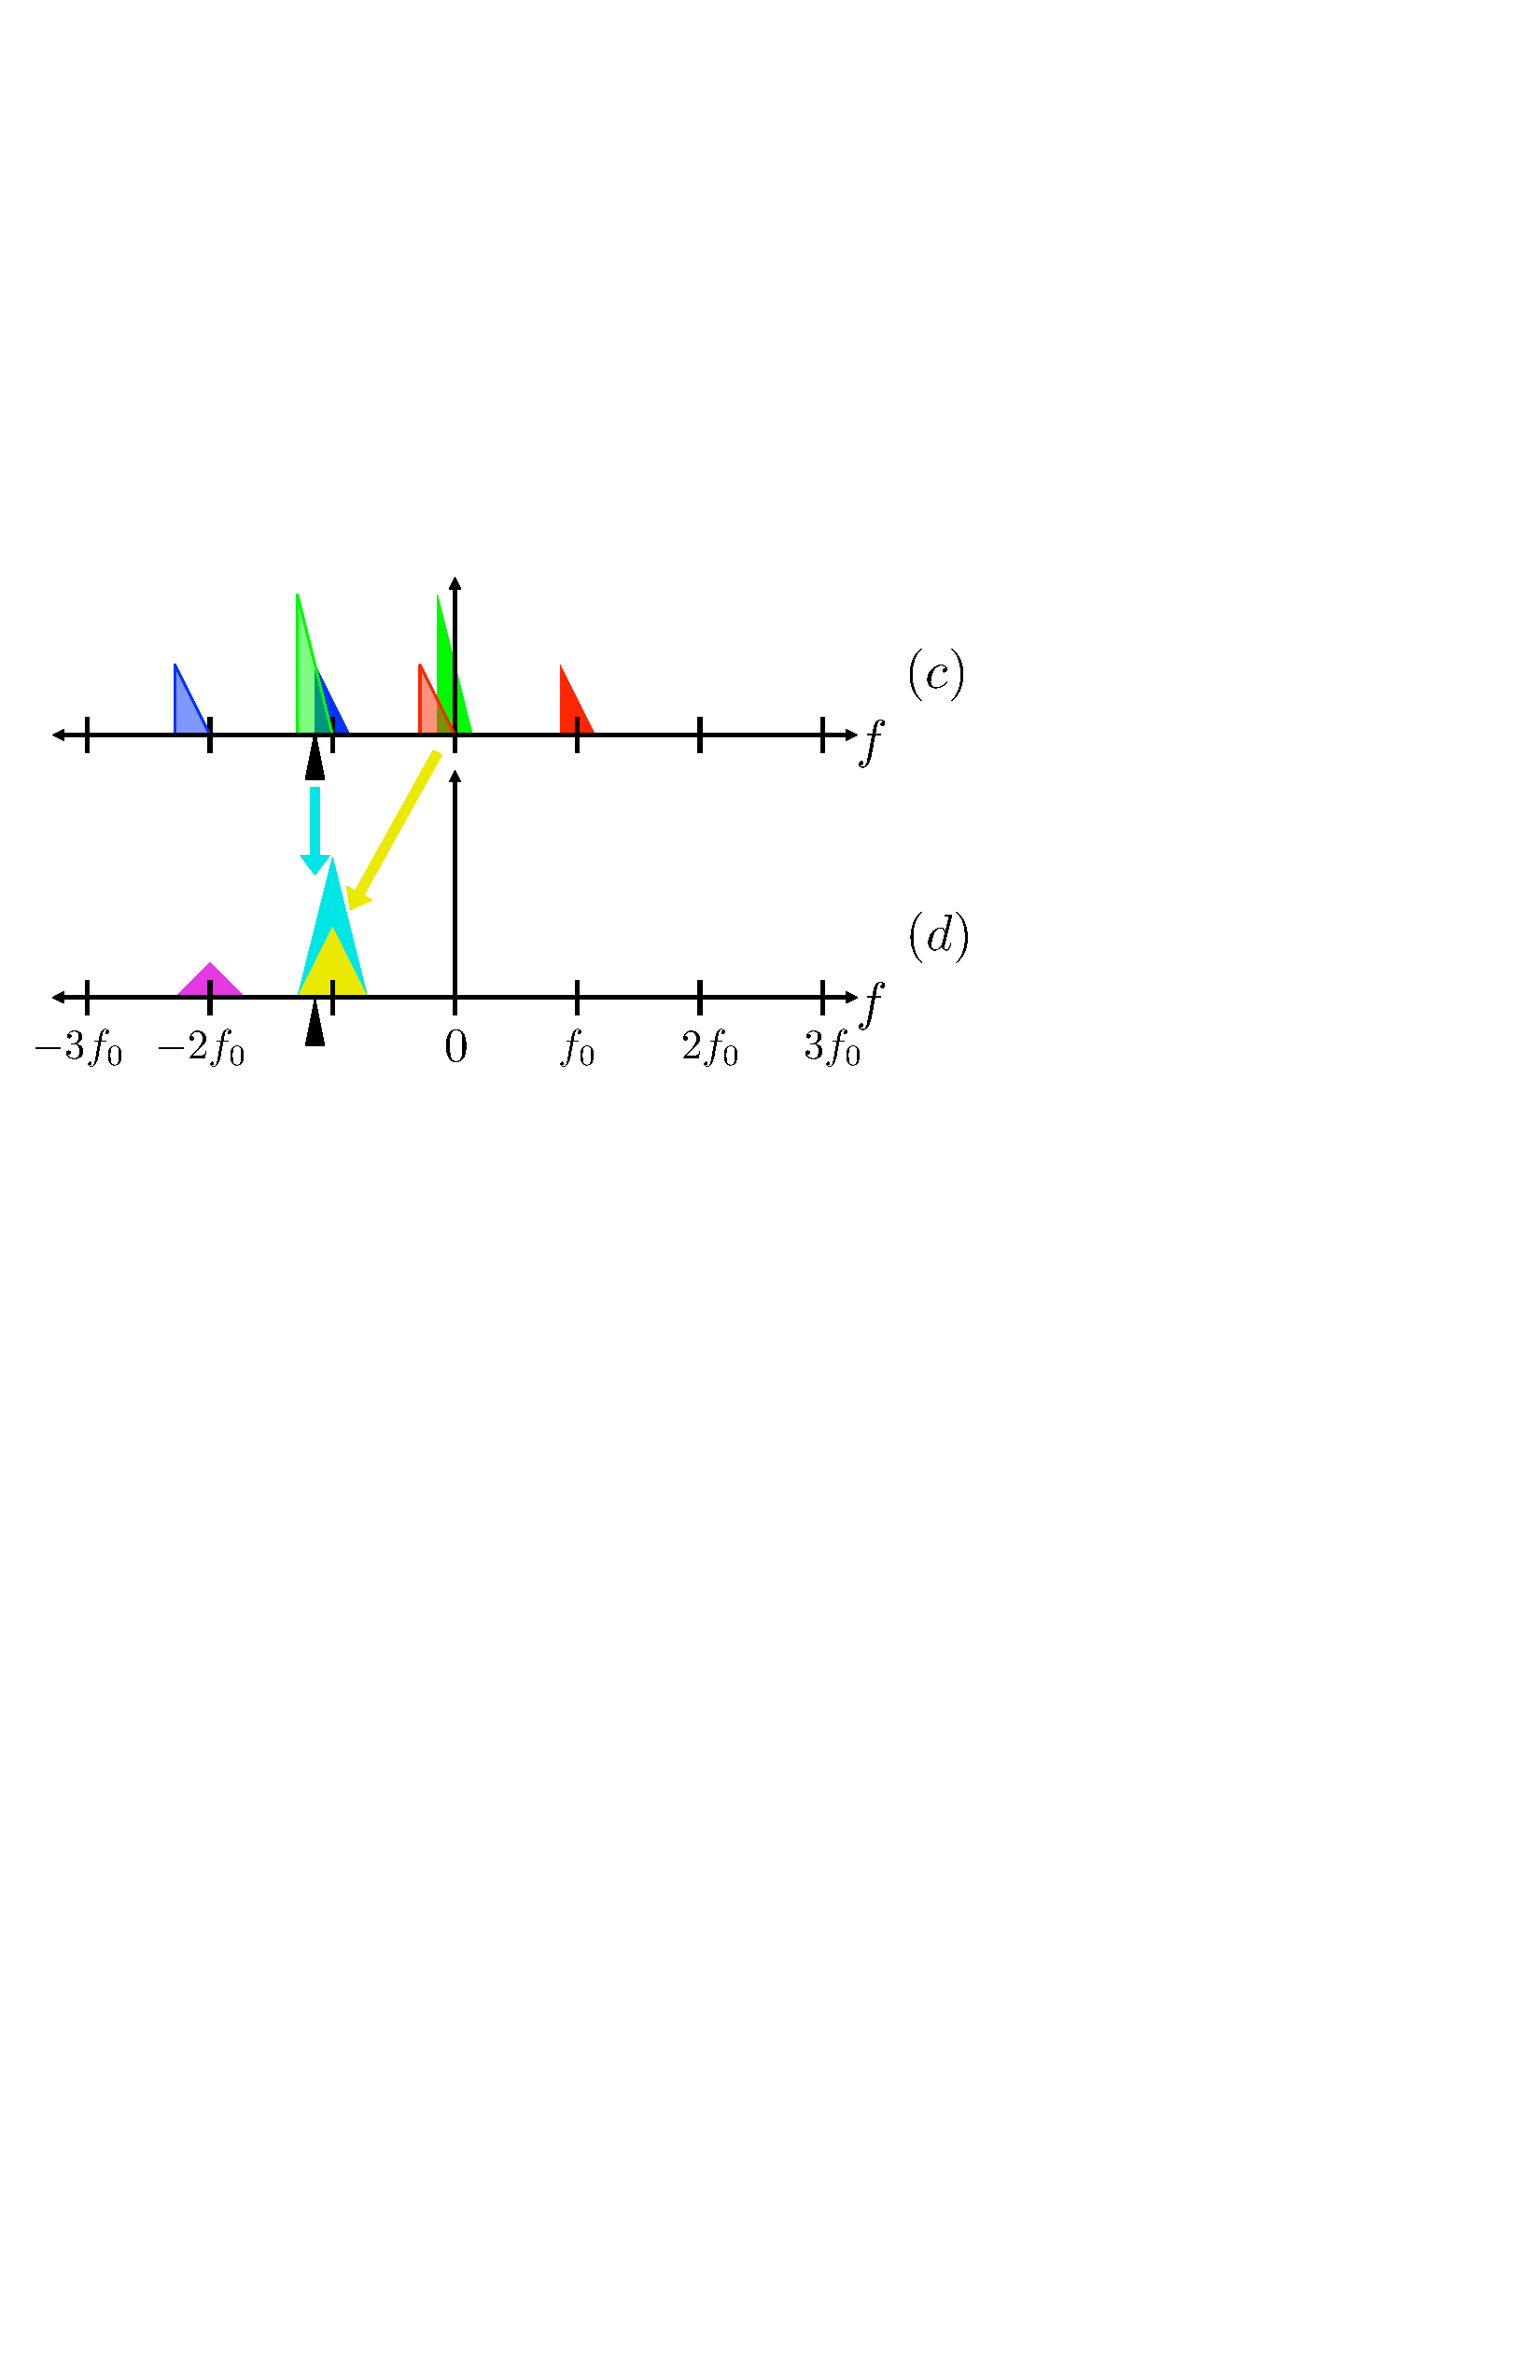
\includegraphics[width=.62\textwidth]{harmonic_envelope_F0} 
    \caption{Envelope Estimate $-F_0$ Component}\label{fig:harmonic_envelope_F0}
    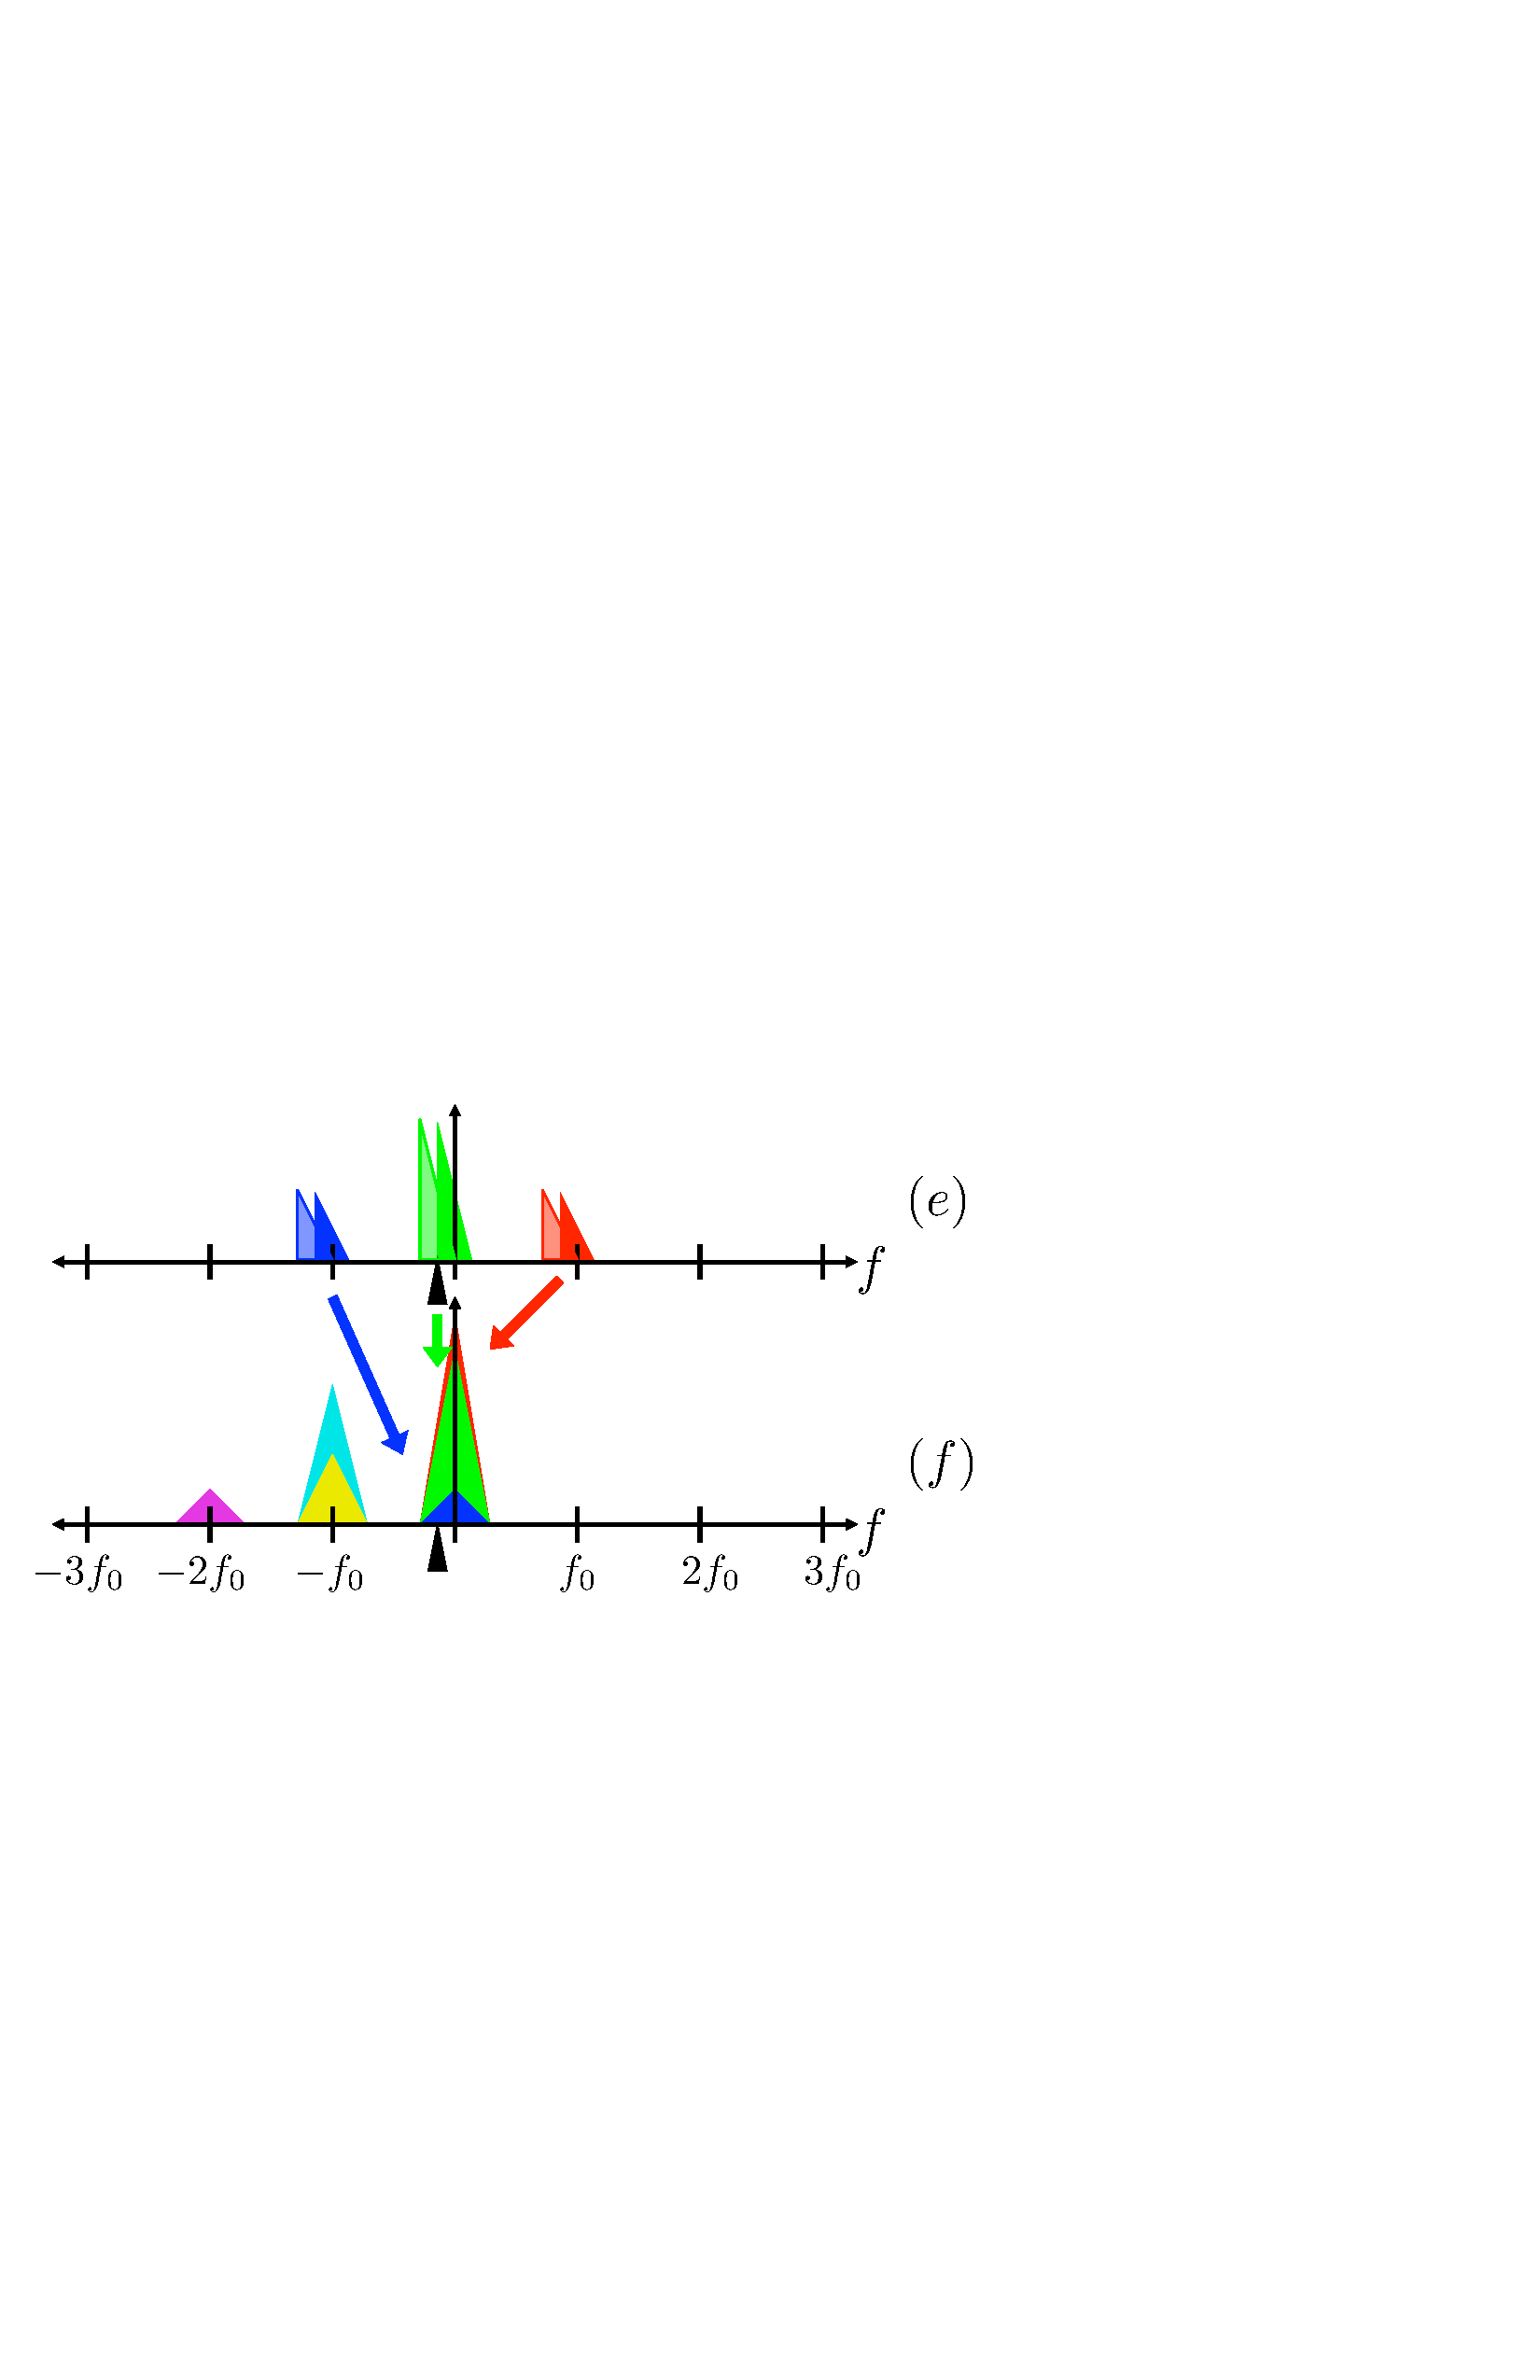
\includegraphics[width=.62\textwidth]{harmonic_envelope_0}
    \caption{Envelope Estimate Baseband Component}\label{fig:harmonic_envelope_0}
\end{figure}

\clearpage

\subsection{2 Harmonic Example: Effects of Downshift Frequency}

We saw clearly in our 3 harmonic example how a non-ideal filter causes distortions in the estimate.  We now visualize the effects of downshift frequency by comparing $F_{DS} = F_0$ to $F_{DS} = F_0 + F_{err}$.

We can see from figure~\ref{fig:downshift_effects} that the non-ideal downshift affects the relative amplitudes of the desired harmonic to interference harmonics when filtering.  As a result the baseband term will be lower amplitude and the terms at multiples of $F_0$ will be higher amplitude.

\begin{figure}[!ht]
  \centering
    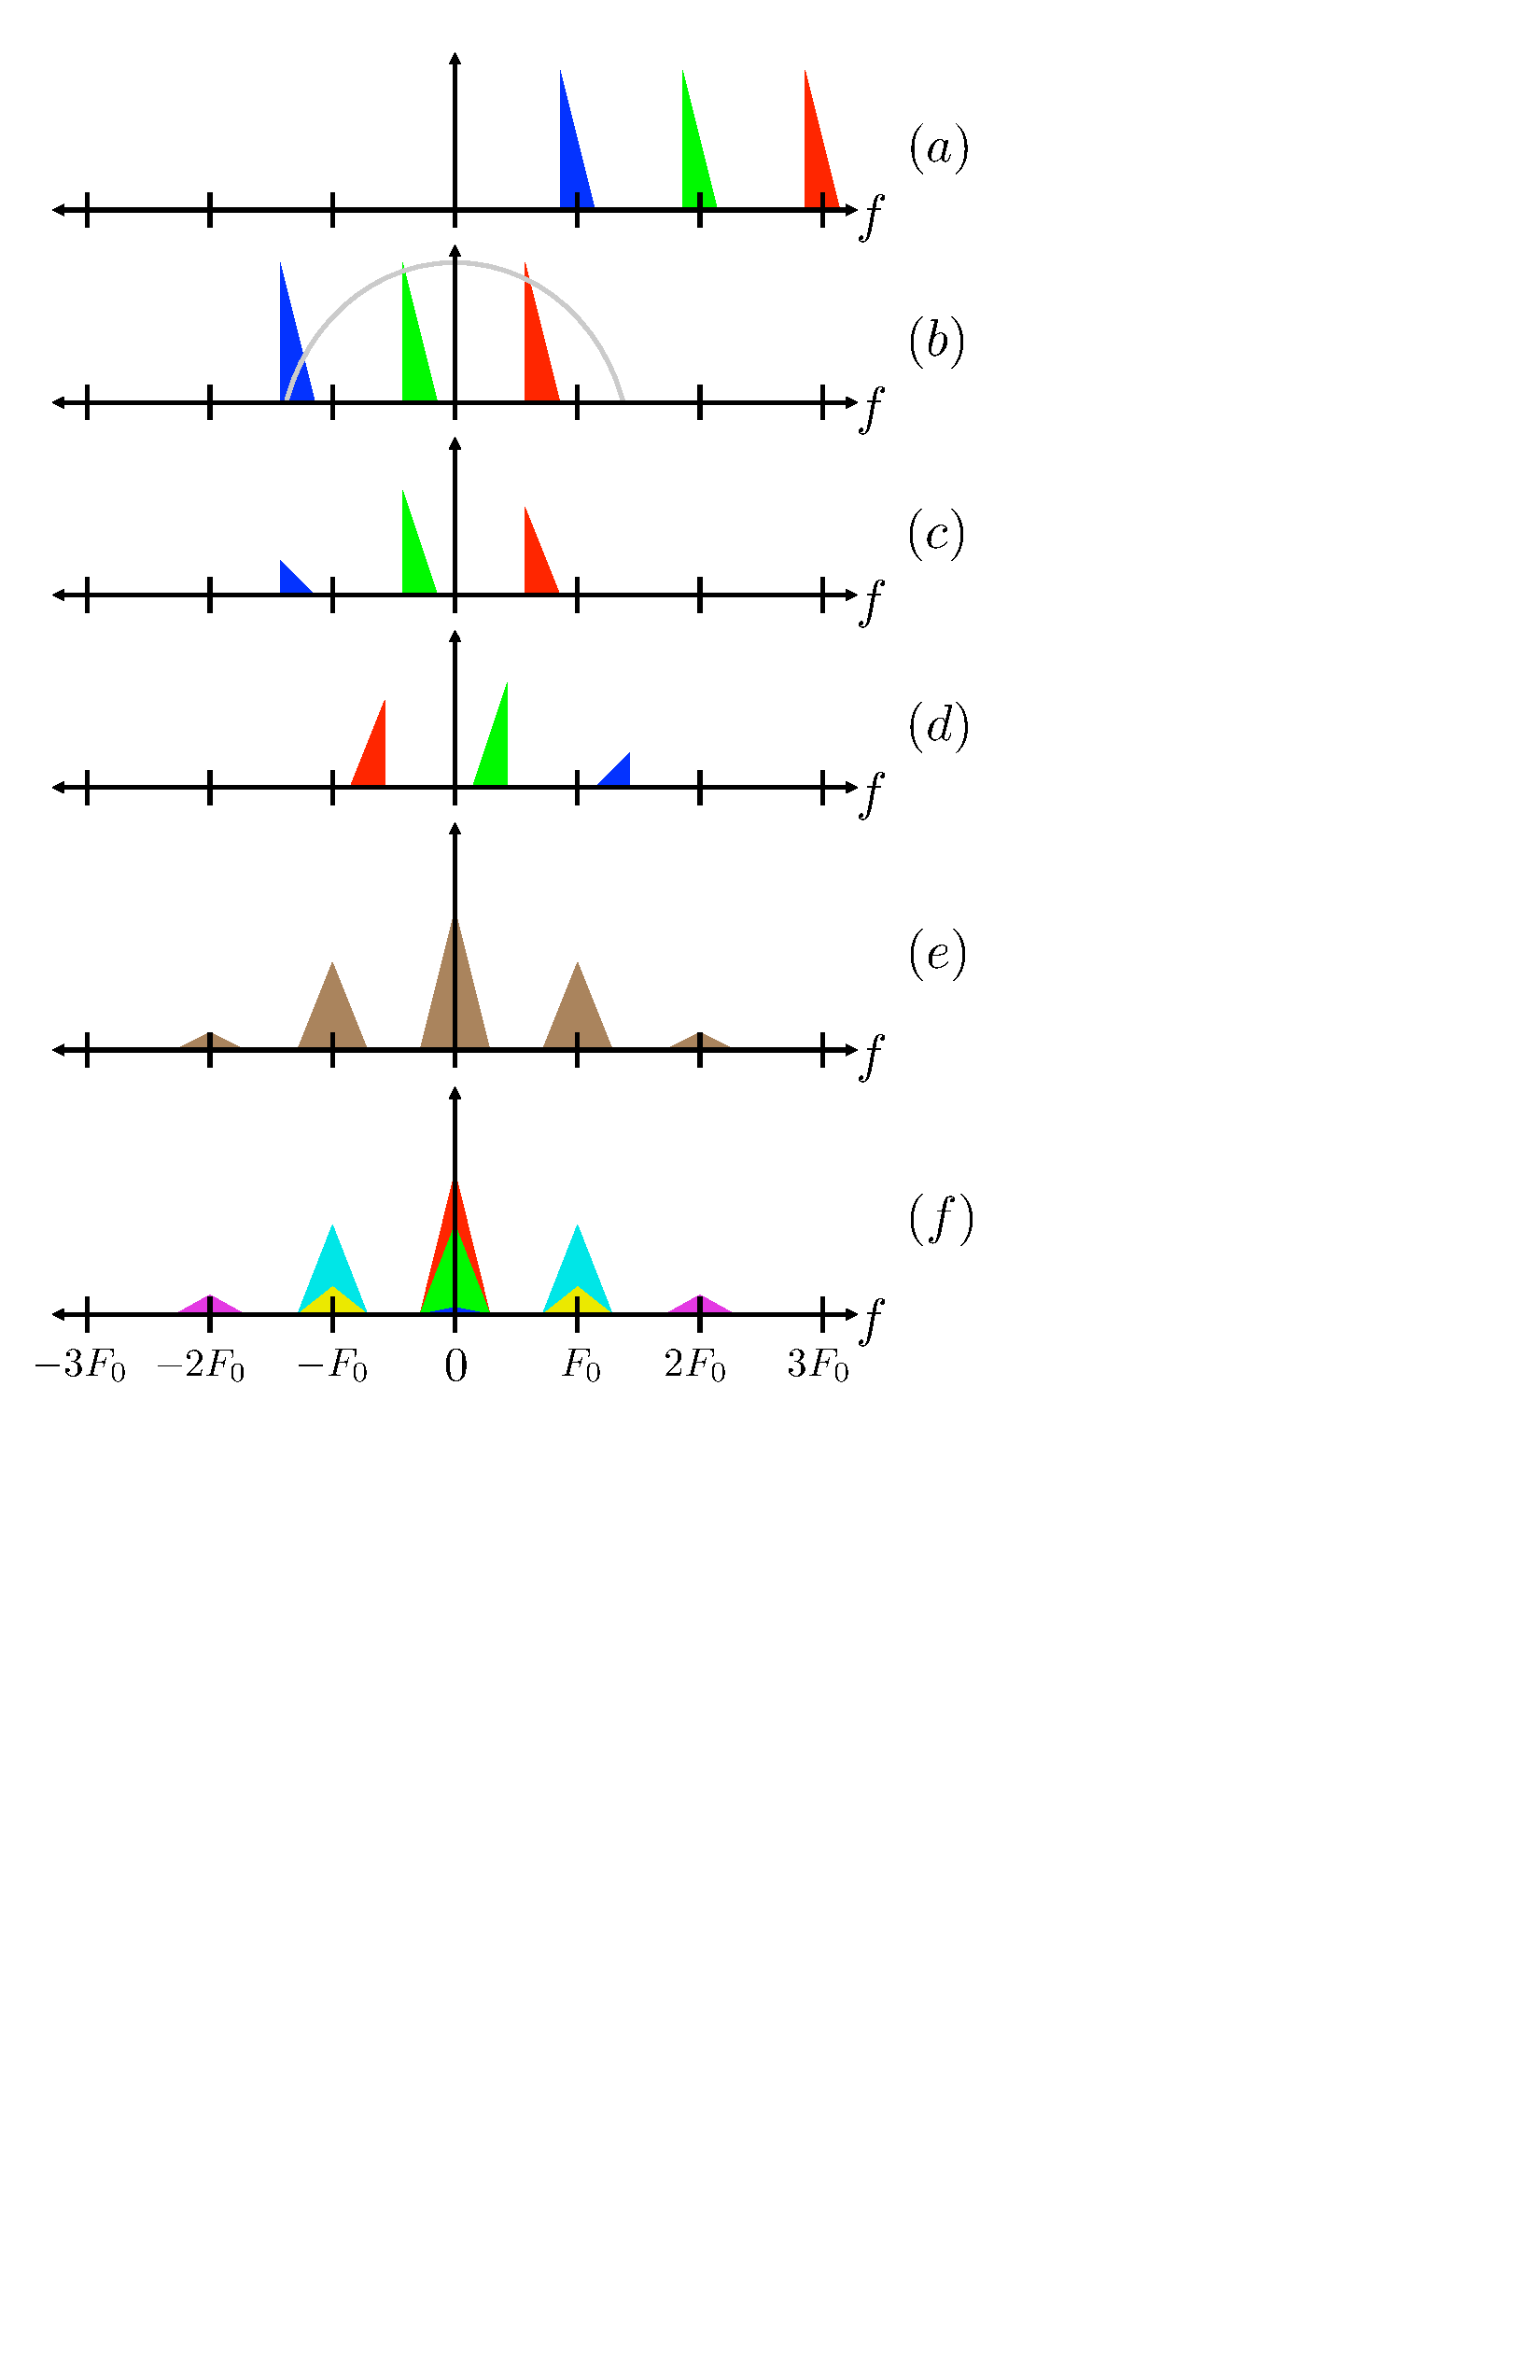
\includegraphics[width=1\textwidth]{downshift_effects} 
    \caption{Comparison of ideal and non-ideal downshift frequencies, faded lines represent ideal
			    $(a) | \widehat{X}[n,f) |$   
    				$(b) | \widehat{X}[n,f - F_{DS}) |$  
				$(c) | H(f) |$
    				$(d) | \widehat{X}[n,f - F_{DS}) | | H(f) |$  
				$(d) | \widehat{X}^*[n,-f + F_{DS}) | | H(-f) |$
				$(e) | \mathcal{F} \{ \tilde{m}_0^2[n] \} |$ }\label{fig:downshift_effects}
\end{figure}

\section{Steady-State Metrics}

In considering how well our envelope $\tilde{m}_k[n]$ estimates $m_k[n]$ there are three important metrics.  We will now discuss each in detail.

\subsection{Coherent Gain}

Coherent gain is defined as the gain of the harmonic of interest, $k$.

\begin{align}
G_k = \Big| H_k\big(e^{j\omega_{k,k}}\big) \Big|
\end{align}

Recalling equation~\ref{eq:downshift_radian_frequency}, if $F_{ds,k} = (k+1)F_0$ then, $w_{k,k} = 0$ and the coherent gain is simply the DC gain of the filter.

\begin{align}
G_k = \Big| H_k(0) \Big| = \sum_n h_k[n]
\end{align}

We may further simplify this by normalizing our filter such that $\Big| H_k(0) \Big| = 1$.  Of course, our downshift frequency won't be ideal in real systems.  Factors to consider include the quantization of $F_{ds,k}$ and the accuracy of $F_0$ estimation.

A similar metric, brought up in [windows for harmonic analysis] is termed scalloping loss, or picket-fence effect.  This is the effect of the harmonic falling in between filter centers.  

%scalloping loss or picket-fence effect, ratio of coherent gain for tone located half a bin from DFT sample point to coherent gain for tone located exactly at sample point

%\begin{align}
%scalloping loss = \frac{| H(\frac{1}{2} \frac{F_s}{N}) |}{H(0)}
%\end{align}

%"althought scalloping loss is useful, it's not entirely informative.  if the scalloping loss if high, then this relates to a sharp cutoff which is actually good for increasing purity of the harmonic"

%worst case processing loss = scalloping loss * PL
%where PL is reduced gain of window (which i have been canceling out)
%**where does worst case processing loss fit in?**

\subsection{Harmonic SIR}

Continuing our focus on the baseband, another question is: what is the contribution of the target harmonic versus the others?  The baseband component is contributed to by spectral leakage due to non-ideal filters.  This is visualized as the red and blue in figure~\ref{fig:harmonic_envelope_0}$(f)$.  The harmonic signal-to-interference-ratio (SIR) quantifies the ratio of target harmonic to spectral leakage.

\begin{align}
SIR_k =& \frac{\Big| H_k\big(e^{j\omega_{k,k}}\big) \Big|} {\Bigg[ \sum\limits_{l=0}^K \Big|H_k\big(e^{j\omega_{k,l}}\big)\Big|^2 \Bigg] ^ \frac{1}{2}}
\end{align}

The terms will roll off as the harmonic center frequencies get further away from $F_{ds,k}$, so typically $SIR_k$ is sufficiently described by only one or two harmonics on either side of the $k$'th, i.e. $k-2 \leq l \leq k+2$.

Harmonic SIR does not describe the true signal-dependent SIR, as varying envelope magnitudes across harmonics will change this, however it does provide an objective measure of the quality of our system to arbitrary harmonic inputs.

% one measure of spectral leakage is asymptotic falloff (db/octave) of sidelobes [windows for harmonic analysis]

\subsection{Modulation Depth}

Finally, we consider the magnitude of each bandpass component relative to baseband.  These terms appear in our envelope estimate as modulations at rates that are multiples of $F_0$.  Because of the forced symmetry of the real envelope we only need to consider positive frequencies, $iF_0$.

\begin{align}
D_{k,i} =& \frac{\Bigg[ \sum\limits_{l=0}^{K-i} \Big|H_k\big(e^{j\omega_{k,l}}\big)\Big| \Big|H_k\big(e^{j\omega_{k,l+i}}\big)\Big|\Bigg]^\frac{1}{2}}
{\Bigg[ \sum\limits_{l=0}^K \Big|H_k\big(e^{j\omega_{k,l}}\big)\Big|^2 \Bigg] ^ \frac{1}{2}}, \quad 1 \leq i \leq K
\end{align}

The largest value and, for that reason, most important value is $D_{k,1}$, the modulation depth at $F_0$.

\section{Induced VS Explicit Temporal Modulation}

So our three metrics are coherent gain, harmonic SIR and modulation depth.  We aim for a coherent gain of $G_k = 1$ and maximized harmonic SIR.

We have mentioned in section~\ref{ss:ACE} that we can have either induced or explicit temporal modulations.  For explicit modulation systems our goal is minimum modulation depth.  For induced that is not as clear.

In this document we argue that the latter, explicit modulation option is better.  The reasoning is best shown by a motivational example.

Let's consider a single note played by two different instruments: clarinet and saxophone.  In this example $F_0 = 261Hz$.  The clarinet is interesting in that it only has energy at odd harmonics.

We attempt to estimate the 3rd harmonic, $m_3[n]$.  We first downshift by $-3F_0$, then lowpass filter.  The spectrum of each signal at this stage is visualized in figure~\ref{fig:clarinetVSsax_F}.  The top panel shows the output of a sufficiently narrow filter where the 3rd harmonic is isolated.  The bottom panel shows a different filter design that intentionally allows the two adjacent harmonics to pass through.  Here we start to see the problem, that despite the wide bandwidth filter, there is (almost) no energy around $\pm F_0$ for the clarinet because of the harmonic structure.  (There is something present however it's down 30dB.)

\begin{figure}[!ht]
  \centering
    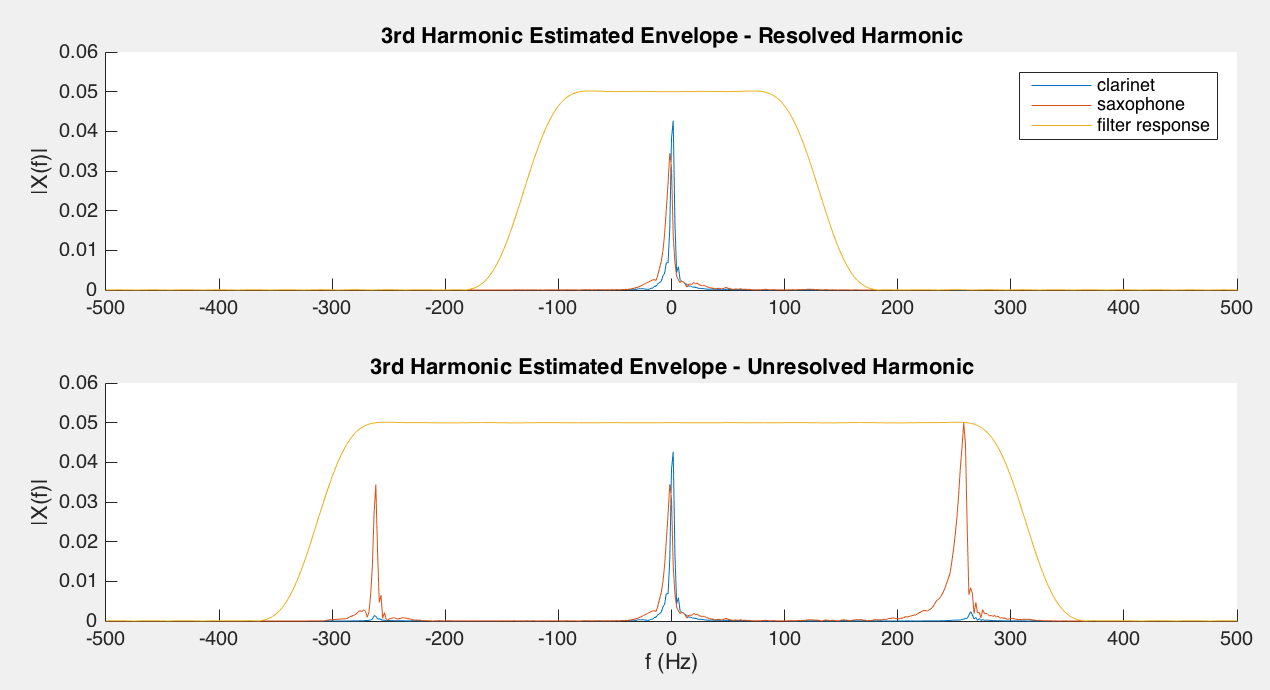
\includegraphics[width=1\textwidth]{clarinetVSsax_F}
    \caption{Clarinet vs Saxophone Harmonic Components}\label{fig:clarinetVSsax_F}
\end{figure}

Figure~\ref{fig:clarinetVSsax_T} shows the time-domain envelopes resulting from this processing.  The input signals were normalized such that the top panel shows the same signal power for both instruments.

The problem is clearly represented in the bottom panel, were we have a very large $F_0$ modulation in the saxophone envelope but little to no change in the clarinet.  The result is that we have a much stronger temporal pitch cue as well as louder overall volume to the saxophone.

\begin{figure}[!ht]
  \centering
    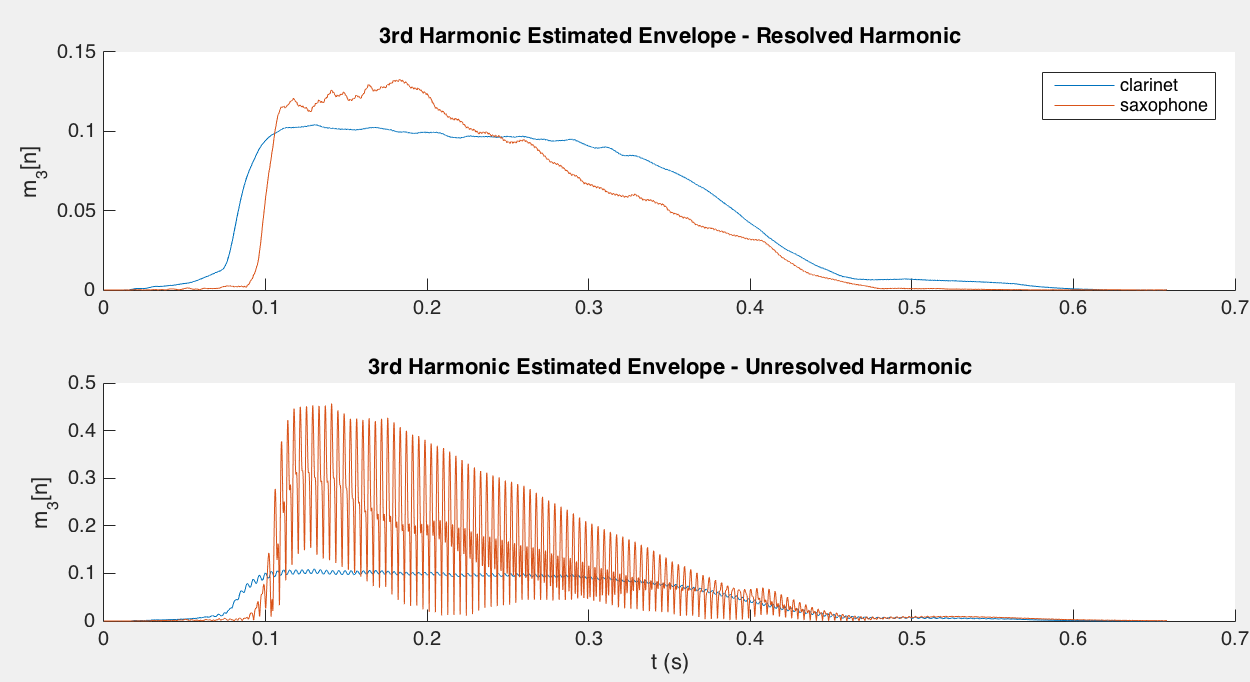
\includegraphics[width=1\textwidth]{clarinetVSsax_T}   
    \caption{Clarinet vs Saxophone Envelope Estimates}\label{fig:clarinetVSsax_T}
\end{figure}

Spectral leakage into other harmonic envelopes is not natural.  It forces the envelope to modulate as a function of the adjacent harmonics which, as we just saw, is signal dependent.  Furthermore, if we have uniform bandwidth filters, (as ACE does), the harmonic resolution will not behave as it does in the cochlea.

Beyond this example, explicit modulation decouples $F_0$ and modulation depth.  This way we have much more control over modulation depth while still making optimal design decisions for envelope extraction.  We can decide modulation depth as a function of how harmonic the signal is.  eTone [REF] uses a harmonic probability metric to do just that.

\subsection{Followup Filter}

Another thing to note is that regardless of downshift frequency, our harmonic envelope will always have it's energy centered at baseband and multiples of $F_0$.  An alternative way of eliminating induced modulations is to add a lowpass filter to the end of the processing chain.

There are a handful of research strategies [REF?] that have used this additional filter.  eTone's envelope follower is an example of this.

The main improvement to a followup filter is that we can guarantee to eliminate temporal modulations.  This could also be achieved by designing a sufficiently narrow filter, $h_k[n]$ however this brings about a tradeoff, where the narrower our filter is the more susceptible we are to error in downshift frequency.

In terms of our three metrics, the followup filter will provide us with a robust coherent gain and guaranteed low modulation depth at the cost of lower harmonic SIR.

Another point to consider is the cost of adding an extra processing stage.  The additional stage means more memory, clock cycles and processing delay.

%On processing delay: The standard ACE strategy has a processing delay equal to half the FFT window duration (i.e., 4 ms). The F0 estimator and envelope tracker stages in eTone introduce an additional delay of 13.75 ms. Previous studies (e.g., Vandali, 2001; Vandali et al., 2005) have shown that delays on this order are not noticed by the majority of CI users. Some how- ever do notice this delay but they quickly become accus- tomed to it. Stone and Moore (2002) observed that for speech production, delays between 25 and 30 ms were dis- turbing. Furthermore for speech perception where lip syn- chronisation is used, delays of around 15–20 ms can become disturbing. The total delay of 17.75 ms is thus just on the border of being unacceptable. [eTone]

% Because of transient smearing, we will not be using this method

\section{Time-Varying F0}

We are only concerned with continuous changes in $F_0[n]$.  Jumps would imply different harmonic envelopes.

$\tilde{m}_k[n]$ uses a window of samples of $\widehat{x}[n]$, equal to the length of $h_k\big[n,F_0[n]\big]$.  If $F_0[n]$ changes significantly within this window we will have problems with our estimate.  That being said, the longest windows considered in the document are 32ms long.  In terms of music, 32ms is equivalent to a sixty-forth note at 120BPM (beats per minute), i.e. very fast.  We will consider this sufficient for typical rates of change of $F_0[n]$.

The other problem that can arise is as $F_0[n]$, our steady-state metrics may change.  This can be evaluated by simply looking at the continuous metrics as a function of $F_0$.

\section{Transients}\label{section:transients}

Nearly everything we have considered so far has suggested the narrower the filter the better.  The problem with this is the time-domain response of filters with fast rolloffs.  There is a tradeoff where the sharper a filter rolls off, the more transient smearing will incur.

Studies on timbre perception [REF?] have suggested that humans hear changes in rise time in the log domain, i.e. the shorter a transient is, the more sensitive our perception is to smearing distortion.

Of course if the pre-processing smears the transients, we can only do as well as that.  Most cochlear implants nowadays use pre-processor dynamic range compression.  We get some insight from a study performed on hearing aids, which would use a similar system.  ``Almost all of the hearing aids tested have attack times less than or equal to 10 ms. A little more than half of the hearing aids had release times of 50 ms or less.  The range of the attack times varied from 1 to 23 ms'' [attack and release times of AGC hearing aids]  1ms is faster than most typical sounds, so we should try to smear transients as little as possible in our processing.

All of this suggests filter bandwidth be as wide as possible without encompassing the other harmonics, which results in a cutoff of $\frac{F_0}{2}$.

% $\frac{1}{5ms} = 200Hz$  Could this plus carrier bandwidth be equivalent to maximum harmonic bandwidth?

%maximum onset dynamic range "90ms - 10ms = 80ms"
%and ratio of filter smeared range to max range
%rinse and repeat for CI's

\section{Evaluation of Strategies}

As stated above the design can be summarized by downshift frequency and lowpass filter.

The ideal downshift frequency is simply $(k+1)F_0[n]$.  The question is what degree of quantization is sufficient to estimate our signal.

For filter design we need to consider bandwidth as a function of filter order and filter/window type.  Ideally our cutoff is somewhere below $F_0$ but high enough to incorporate the bandwidth of $m_k[n]$.

The filters can be different as a function of $k$.  This is a natural path to pursue if we consider the critical bands of the cochlea.  This will be discussed in more detail later in this document however for now we will assume $h_k[n] = h[n]$.  This is natural for harmonic envelopes as harmonics are linearly spaced.

The designs considered are:

downshift quantization - 1, 31, 63, 125Hz

filter order - 128, 256, 512

filter - rectangular, hanning, adaptive hamming

k - which harmonic, how do they relate to each other

Adaptive hamming is an adaptive bandwidth filter with a lowpass cutoff (-6dB point) of $\frac{F_0[n]}{2}$.

For practical considerations, we will set a maximum quantization as $F_s$ /  filter order.

$order = 256 \longleftrightarrow$ $f_q \leq 63Hz$

$order = 512 \longleftrightarrow$ $f_q \leq 31Hz$

We consider only fundamental frequencies in the range of 50-550Hz. This range encompasses the adults and children which are predominantly within 80-300Hz [REF] and it provides some extra range for musical instruments.% [pitch_ranking_strategy_compare]

\subsection{Coherent Gain}

We first look at different downshift quantizations, all else constant.  This is visualized in figure~\ref{fig:g_k_1}.  When $F_0$ is exactly at a quantized value, $G_k = 0dB$, however the gain decreases as $F_0$ drifts away until the worse case where it is exactly in between quantization values.  Decreasing the quantization increases the number of dips and in turn improves the worst case $G_k$.

\begin{figure}[!ht]
  \centering
    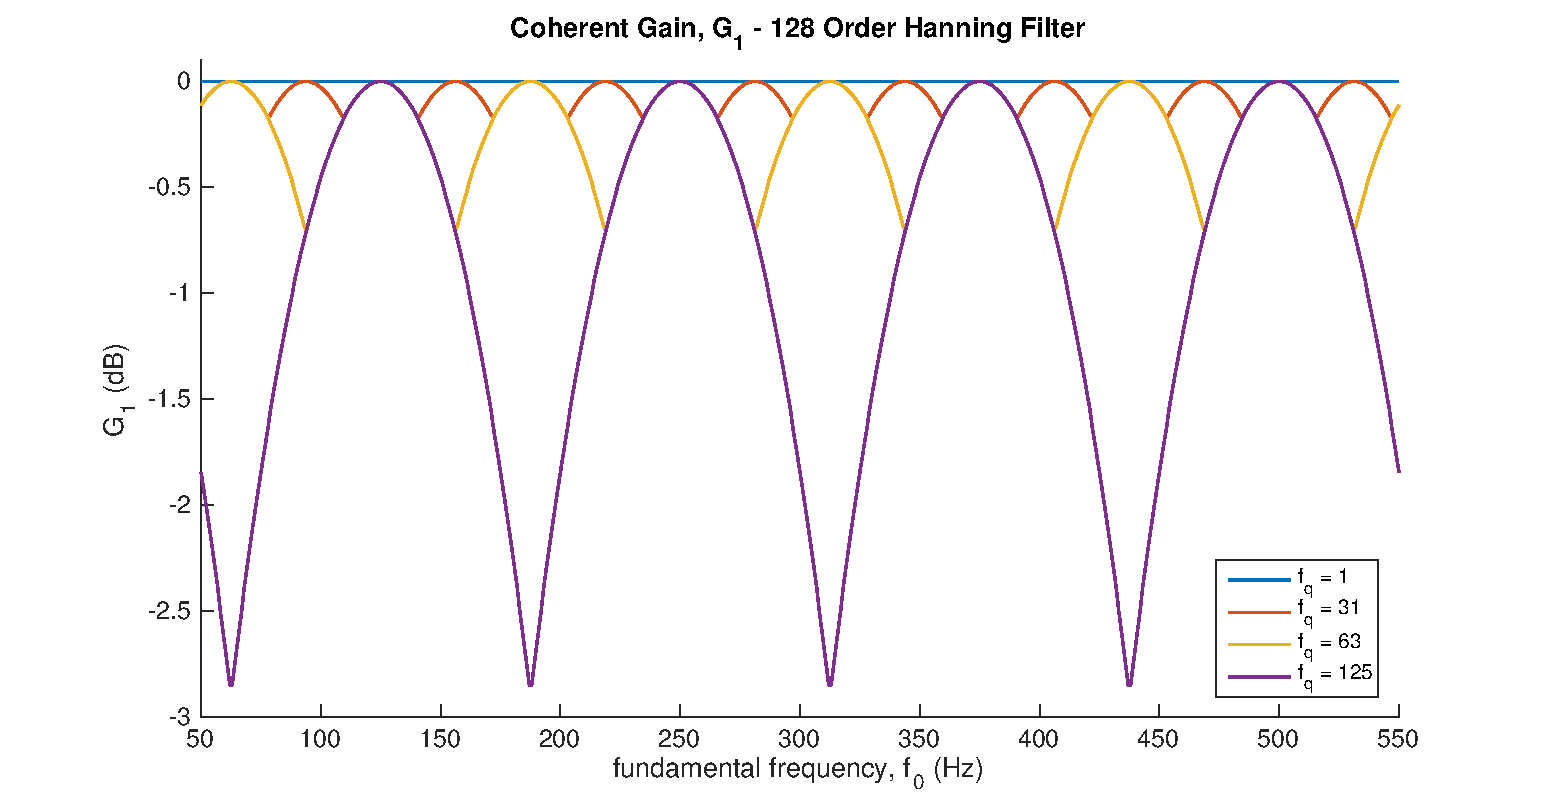
\includegraphics[width=1\textwidth]{g_k_1}   
    \caption{$G_k$ Downshift Quatization}\label{fig:g_k_1}
\end{figure}

Figure~\ref{fig:g_k_2} compares the three different filter orders.  Using a hanning window, the lower order filters have slower rolloffs and better worst case $G_k$.  This doesn't necessarily hold true for adaptive filters.  Provided a high enough desired cutoff that the 128 order filter can achieve this reasonably well, the order become irrelevant.

\begin{figure}[!ht]
  \centering
    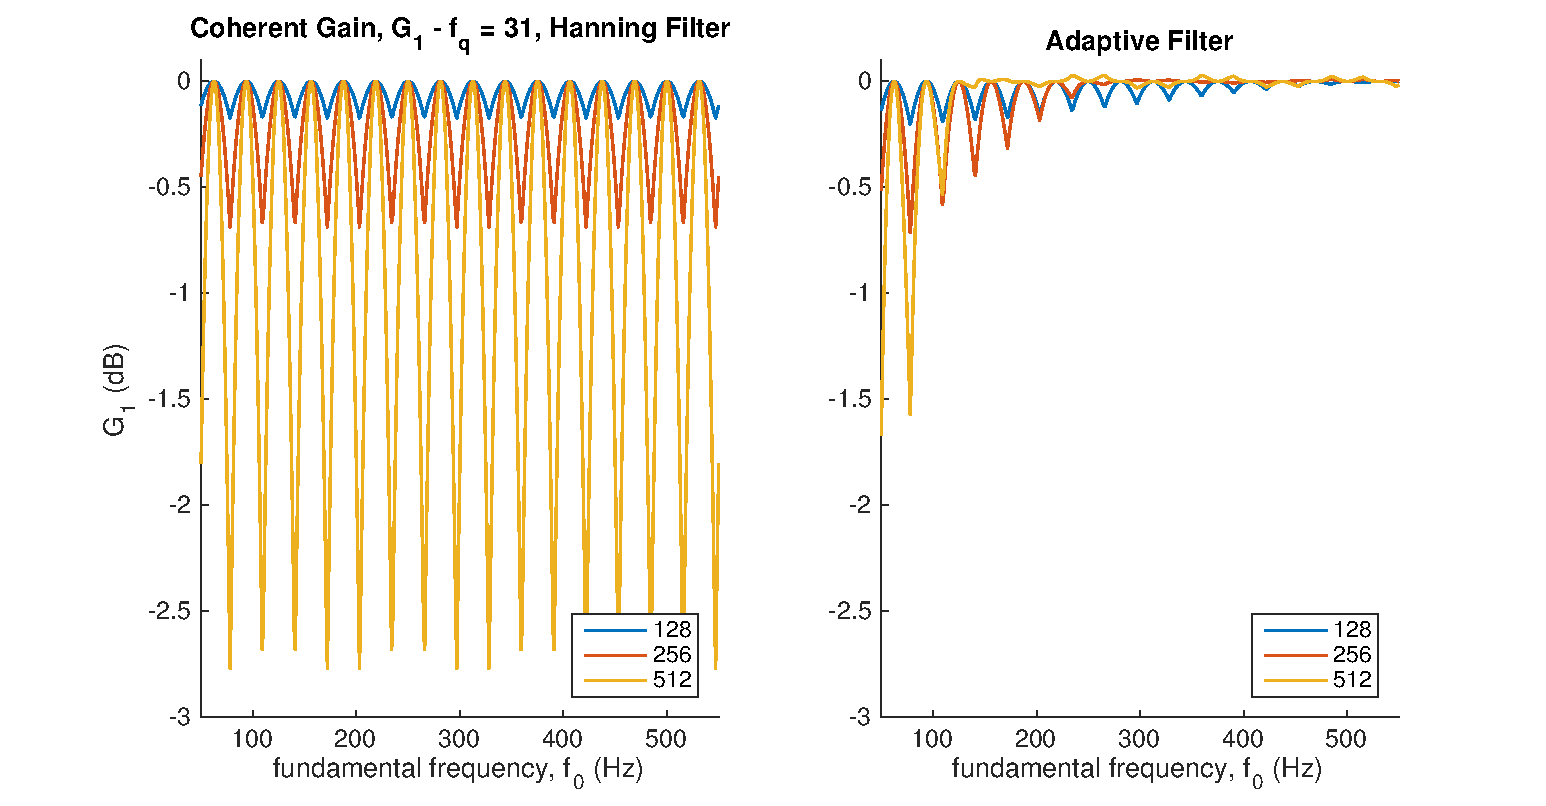
\includegraphics[width=.8\textwidth]{g_k_2}   
    \caption{$G_k$ filter order}\label{fig:g_k_2}
\end{figure}

Figure~\ref{fig:g_k_3} compares the different filter designs.  The wider bandwidth filters have smoother $G_k$ across $F_0$ and as a result the adaptive bandwidth becomes optimal at high $F_0$'s.

\begin{figure}[!ht]
  \centering
    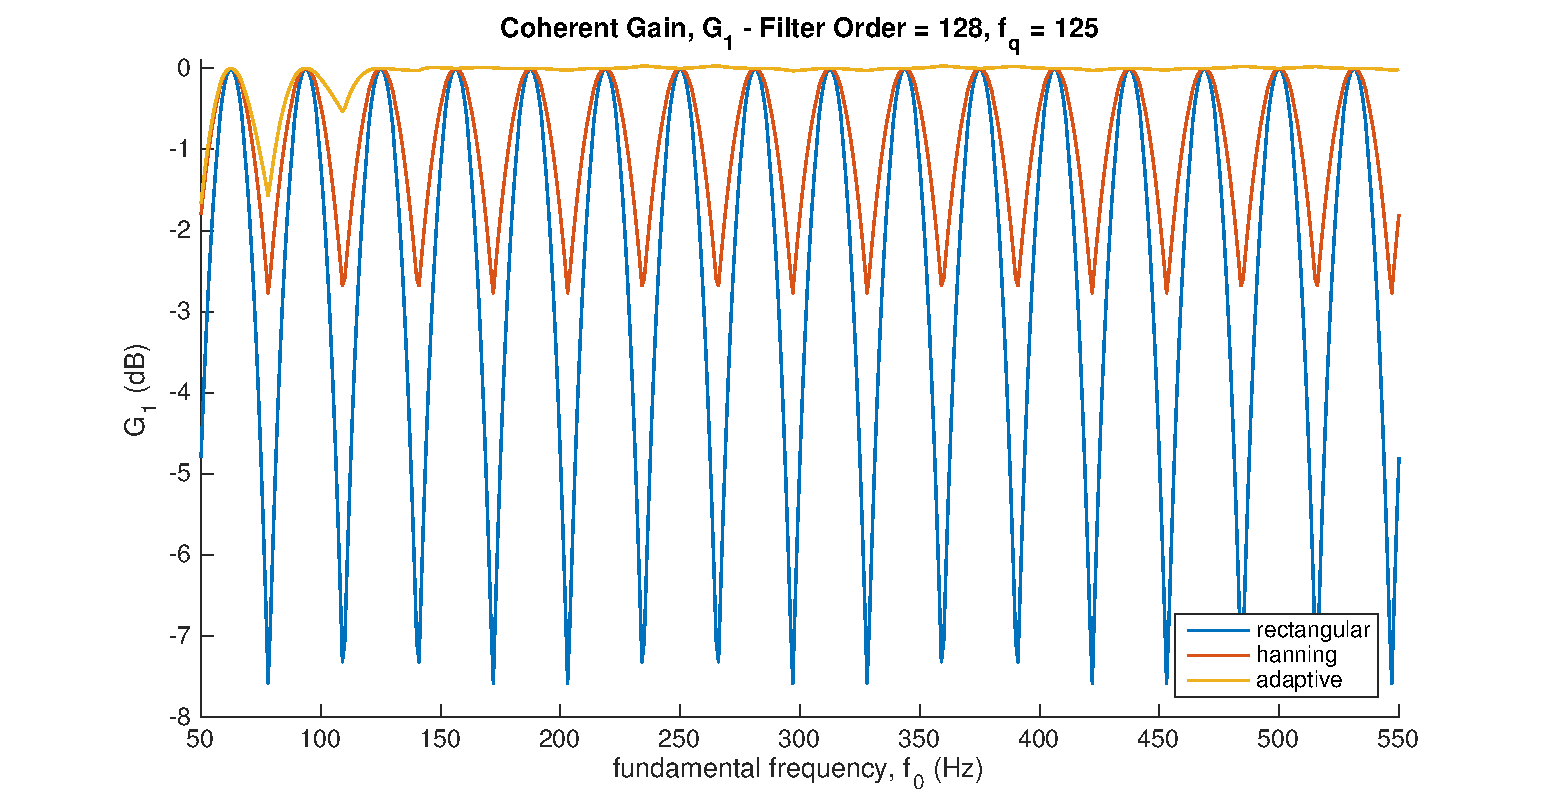
\includegraphics[width=.8\textwidth]{g_k_3}   
    \caption{$G_k$ filter design}\label{fig:g_k_3}
\end{figure}

So lower quantization and wider bandwidth both improve $G_k$, but that's pretty intuitive.  The interesting part here is the relationship between harmonics.  If we consider the first three harmonics, figure~\ref{fig:g_k_4} shows that the number of dips is proportional to $k$.  As a result we get interactions at certain values of $F_0$.  For example, if $F_0 = 1.5f_q = 188$Hz, odd harmonics will be at a minimum and even harmonics will be at a maximum.  This results in a distortion between harmonics where some are attenuated more than others.

It should be noted that pre-processing compression or automatic gain control (AGC) will cause harmonic distortions.  This could arguably be used to either make the case that it is important to minimize further distortions, or alternatively that these further distortions are minimal in comparison and thus shouldn't be over engineered.

\begin{figure}[!ht]
  \centering
    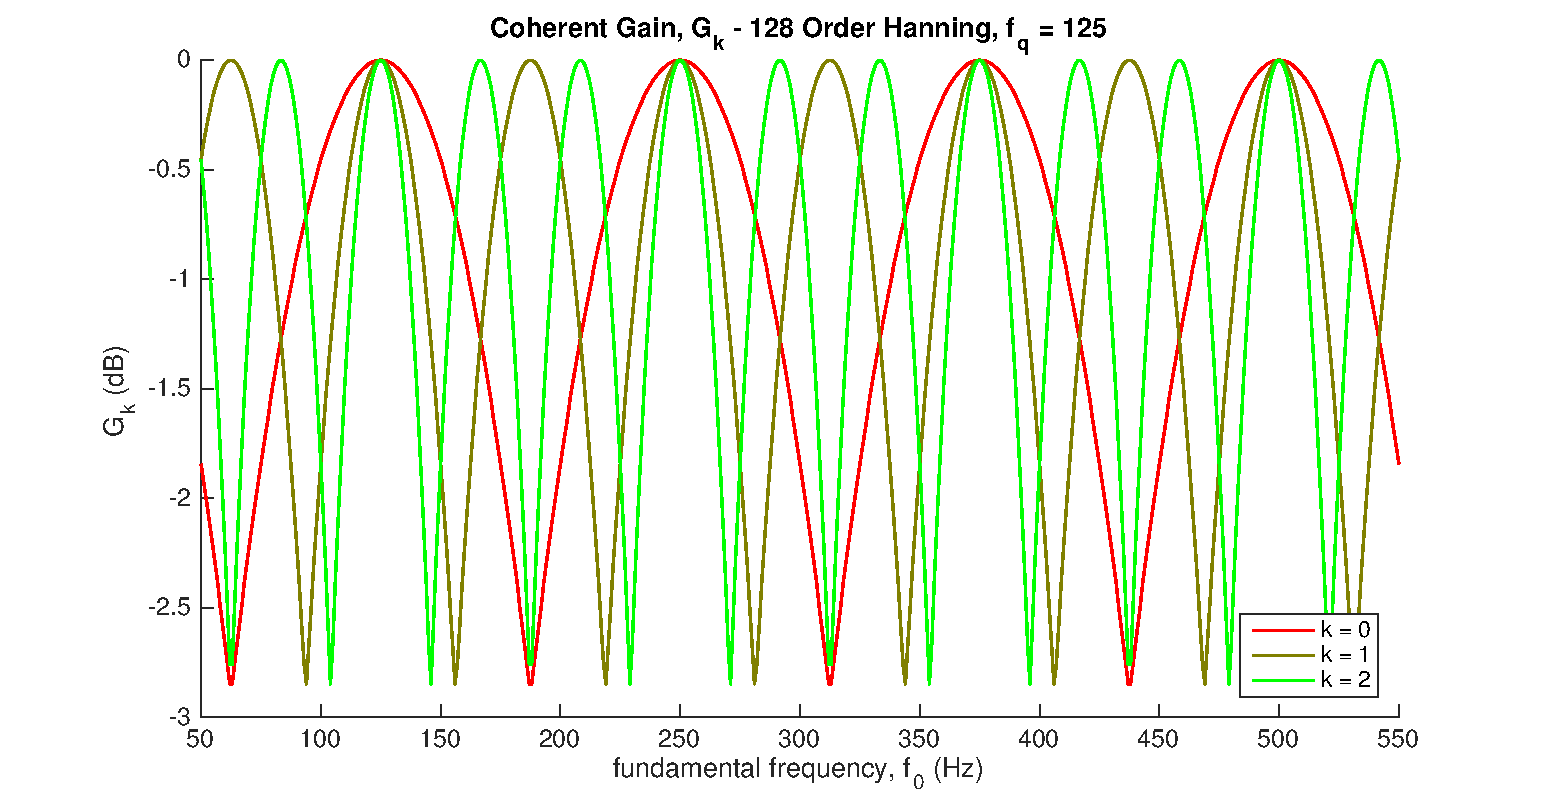
\includegraphics[width=1\textwidth]{g_k_4}   
    \caption{$G_k$ variation across harmonics}\label{fig:g_k_4}
\end{figure}

Considering maximum quatization is $F_s$ / order and hanning filter as our baseline, worst case: $G_k \approx -1.5dB$.  Increasing the filter order and decreasing quantization proportionally increases the number of dips while keeping depth the same.  The relationship between harmonics and the case of $F_0[n]$ continuously changing over time put emphasis on minimizing the dynamic range of $G_k$.

%scalloping loss or picket-fence effect, ratio of coherent gain for tone located half a bin from DFT sample point to coherent gain for tone located exactly at sample point

%\begin{align}
%scalloping loss = \frac{| H(\frac{1}{2} \frac{F_s}{N}) |}{H(0)}
%\end{align}

%"althought scalloping loss is useful, it's not entirely informative.  if the scalloping loss if high, then this relates to a sharp cutoff which is actually good for increasing purity of the harmonic"

%worst case processing loss = scalloping loss * PL
%where PL is reduced gain of window (which i have been canceling out)
%**where does worst case processing loss fit in?**

\clearpage

\subsection{Harmonic SIR}

We first consider filter order and quantization.  In figure~\ref{fig:sir_k_1} we consider all filter orders with and without quantization.

The downshift quandization doesn't actually affect performance significantly.  This can be seen in figure~\ref{fig:sir_k_1} by looking at the two lines corresponding to order = 128.  Above a $F_0 = 250$Hz the harmonics are spaced far enough apart that the quantization doesn't matter.  Below $F_0 = 130$Hz the filter cutoff is not sharp enough to isolate the harmonic, in which case downshift quantization is irrelevant.

Also note that for order = 512 the cutoff is narrow enough that we get ideal harmonic SIR over all $F_0$.

\begin{figure}[!ht]
  \centering
    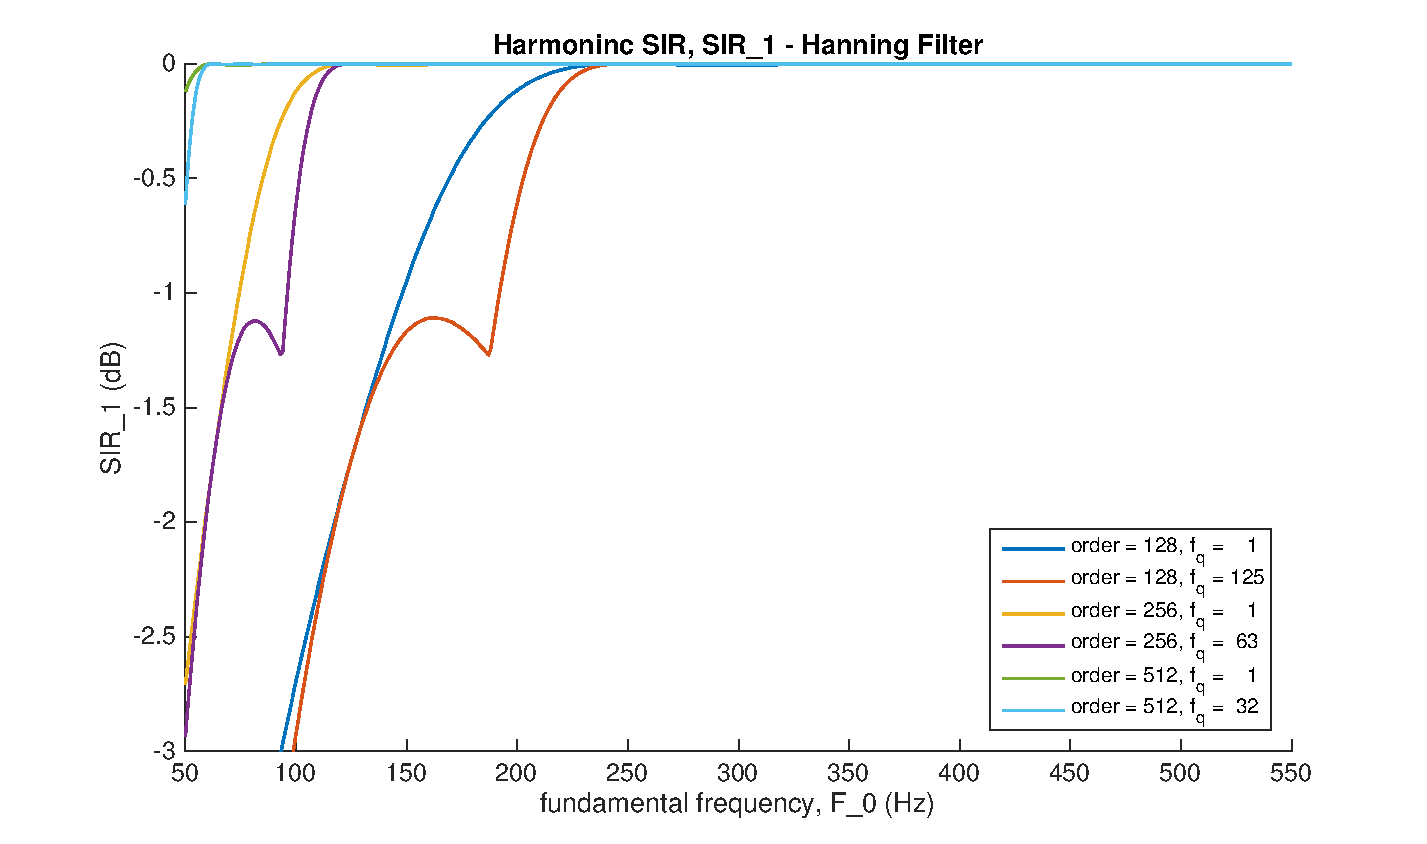
\includegraphics[width=1\textwidth]{sir_k_1}   
    \caption{$SIR_k$ filter order and quantization}\label{fig:sir_k_1}
\end{figure}

Figure~\ref{fig:sir_k_2} compares filter design methods.  Hanning and adaptive are essentially the same, showing that the limiting factor is still filter order.  Rectangular provides a better lower limit for what $F_0$ the SIR breaks down at, and it does this at the cost of dips at higher frequencies.  This agrees with the fact that rectangular windows have the sharpest rolloff at the expense of large sidelobes.

\begin{figure}[!ht]
  \centering
    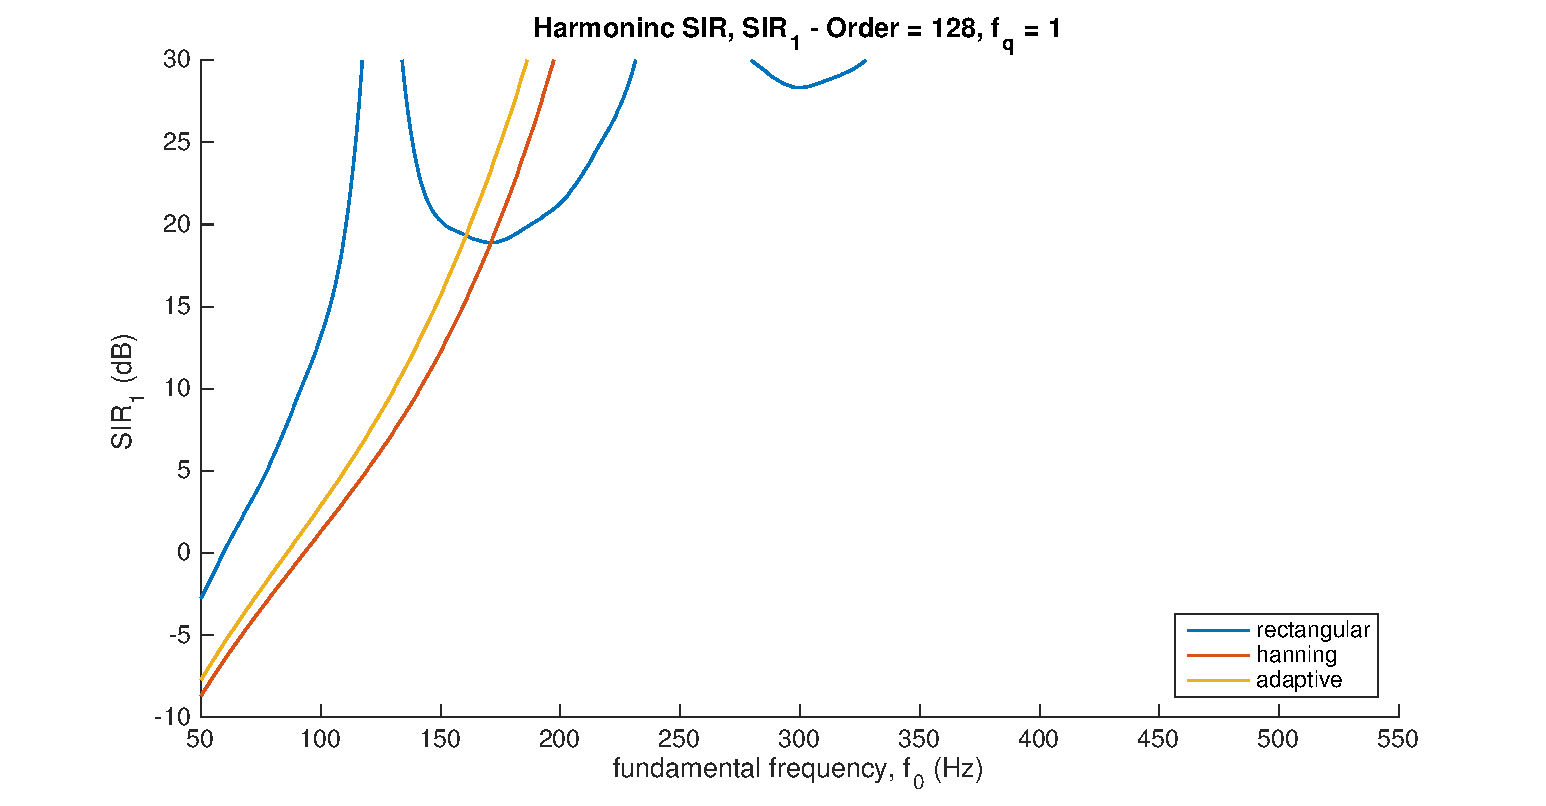
\includegraphics[width=1\textwidth]{sir_k_2}
    \caption{$SIR_k$ filter design}\label{fig:sir_k_2}
\end{figure}

The higher order harmonics are compared in figures~\ref{fig:sir_k_3} and ~\ref{fig:sir_k_4}.  We see patterns similar to figure~\ref{fig:g_k_4} where the number of dips is proportional to $k$.  These figures reinforce that improvement from decreasing quantization, $f_q$, is bounded.

For hanning the incremental 1dB of improvement is arguably not important.  For rectangular we actually see a significant improvement in the 80-130Hz region for $k > 3$.

\begin{figure}[!ht]
  \centering
    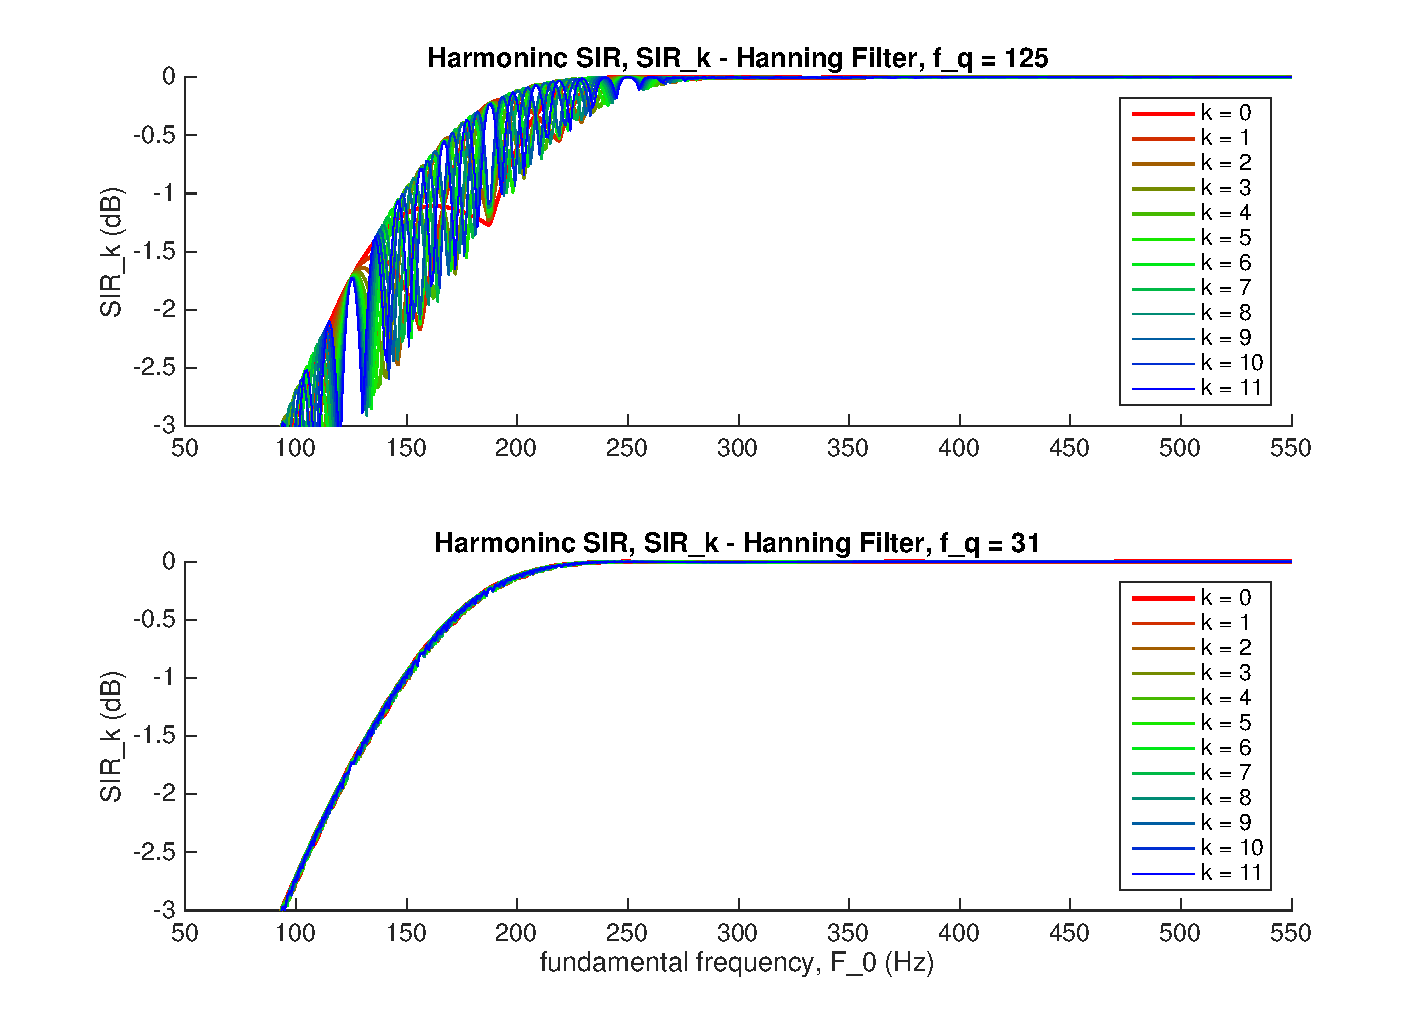
\includegraphics[width=.8\textwidth]{sir_k_3}
    \caption{$SIR_k$ variation across harmonics with hanning filter}\label{fig:sir_k_3}
\end{figure}

\begin{figure}[!ht]
  \centering
    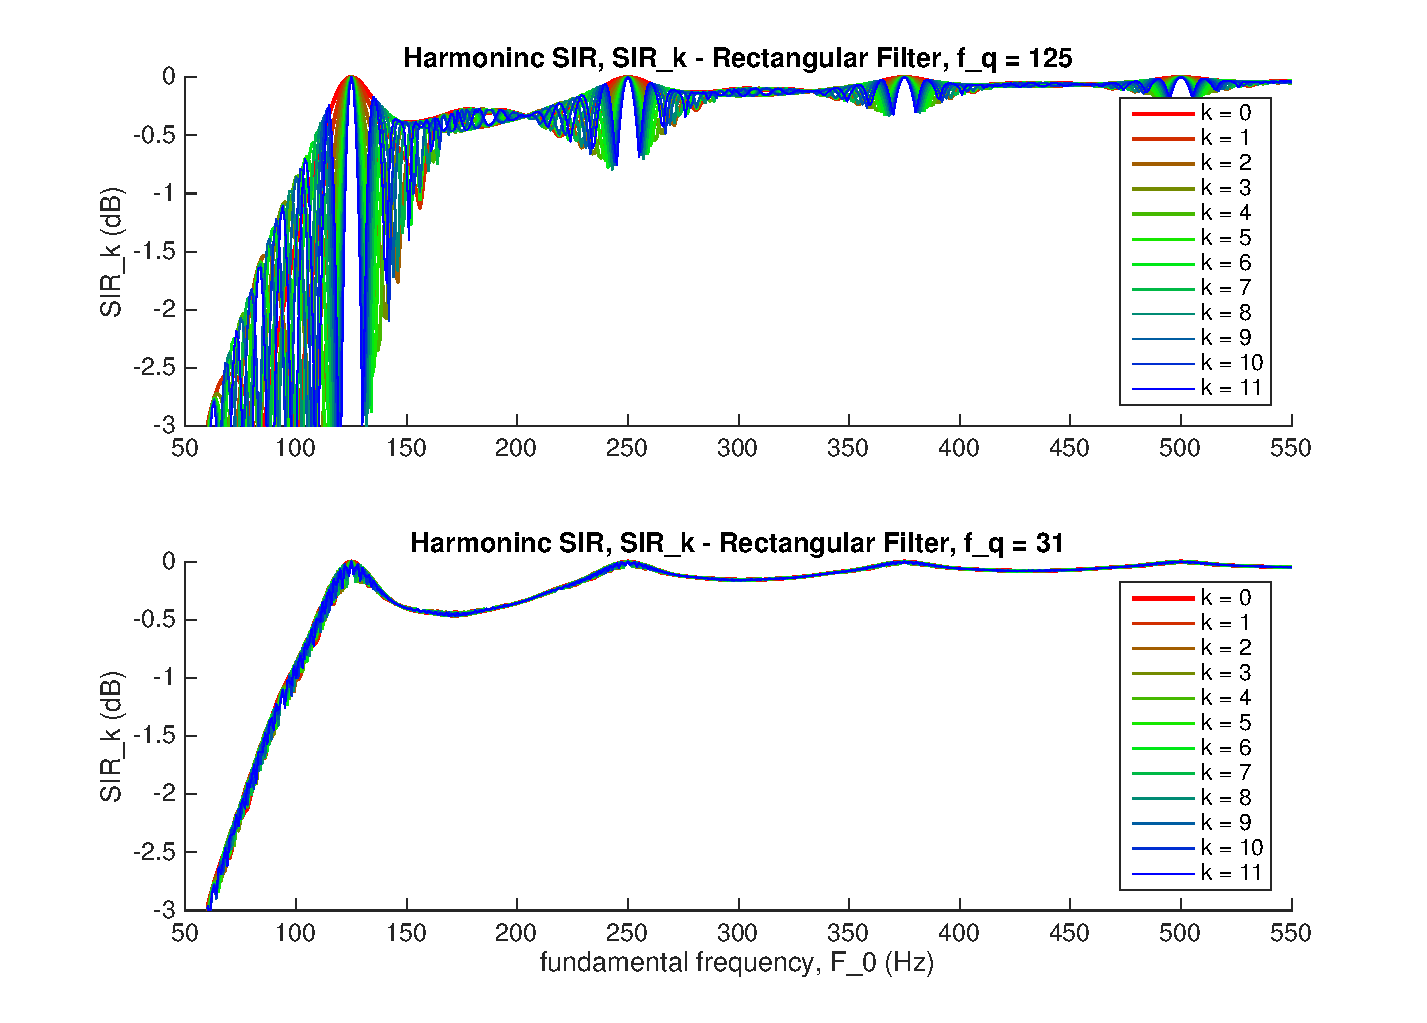
\includegraphics[width=.8\textwidth]{sir_k_4}   
    \caption{$SIR_k$ variation across harmonics with rectangular filter}\label{fig:sir_k_4}
\end{figure}

Filter order is certainly the dominant factor for harmonic SIR.  For order = 128, it starts to break down for $F_0 \approx 220$ Hz and degrades as $F_0$ decreases.  For order = 256, it starts to break down for $F_0 \approx 110$ Hz.  For order = 512 the harmonic SIR performs is essentially optimal across all values of $F_0$.

\clearpage

\subsection{Modulation Depth}

We discussed earlier that our goal is to provide explicit modulations, in which case we need minimal modulation in the extracted envelope.

We first compare each filter design method at the different filter orders, as seen in figure~\ref{fig:d_ki_1}.  For all orders rectangular windows do a poor job of suppressing modulations due to high sidelobe amplitude.  Hanning and adaptive show similar responses with the dominant variation being the response to low $F_0$ as a function of filter order.

\begin{figure}[!ht]
  \centering
    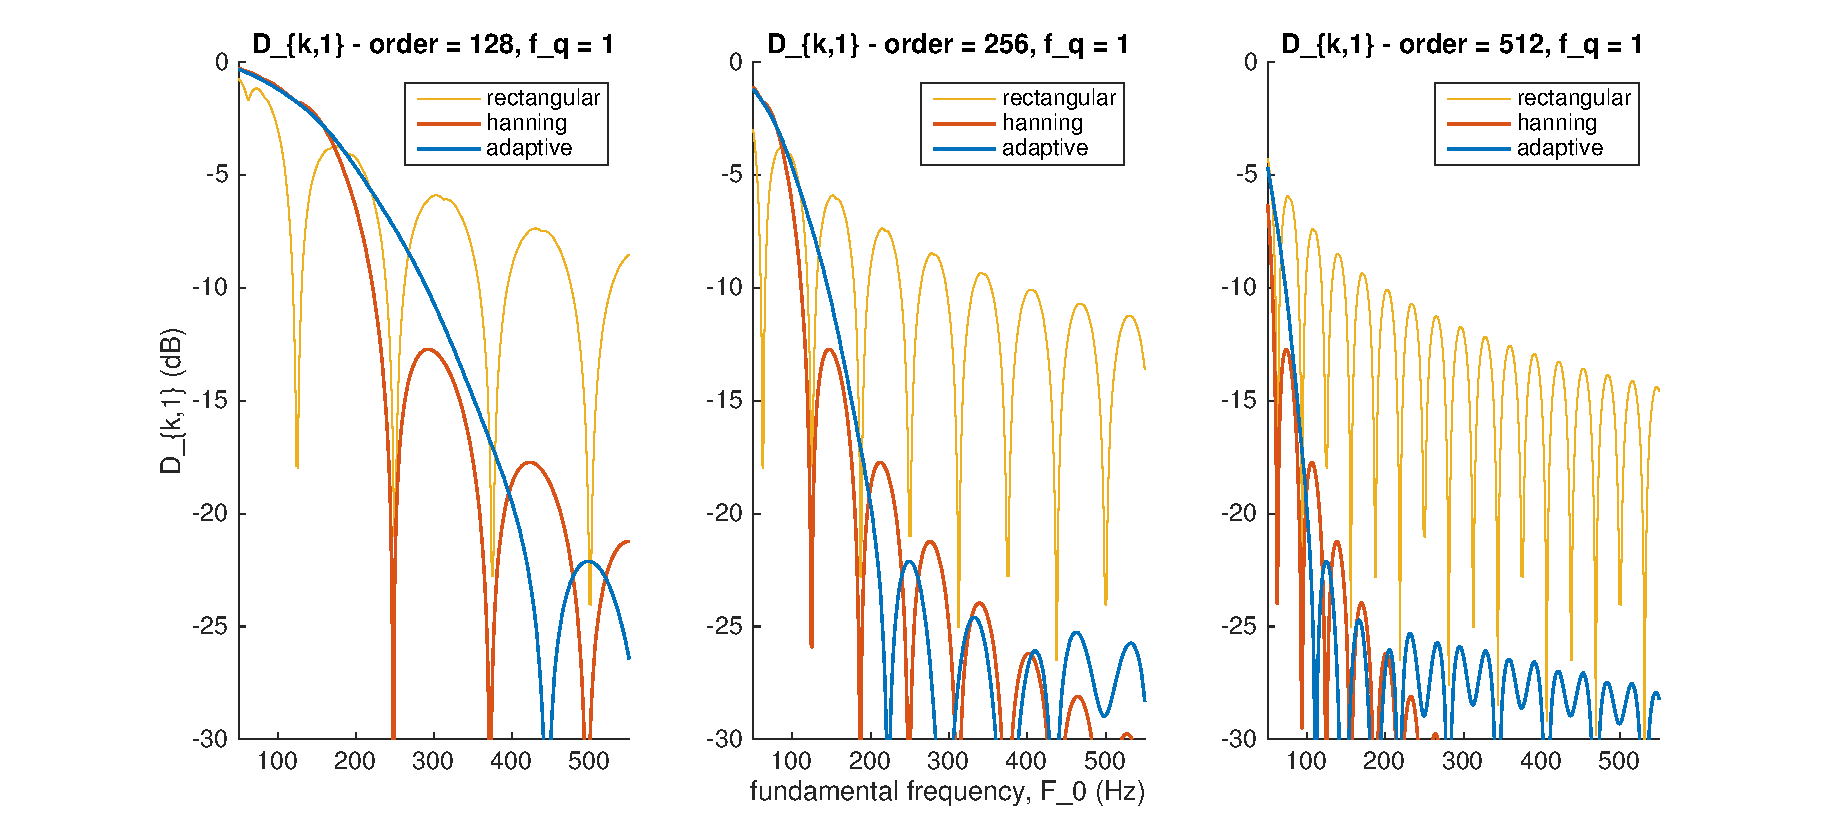
\includegraphics[width=1\textwidth]{d_ki_1}   
    \caption{$D_{k,i}$ filter design and order}\label{fig:d_ki_1}
\end{figure}

Downshift quantization shows little affect on modulation depth.  This is shown for both hanning and adaptive filter designs in figure`\ref{fig:d_ki_2}.

\begin{figure}[!ht]
  \centering
    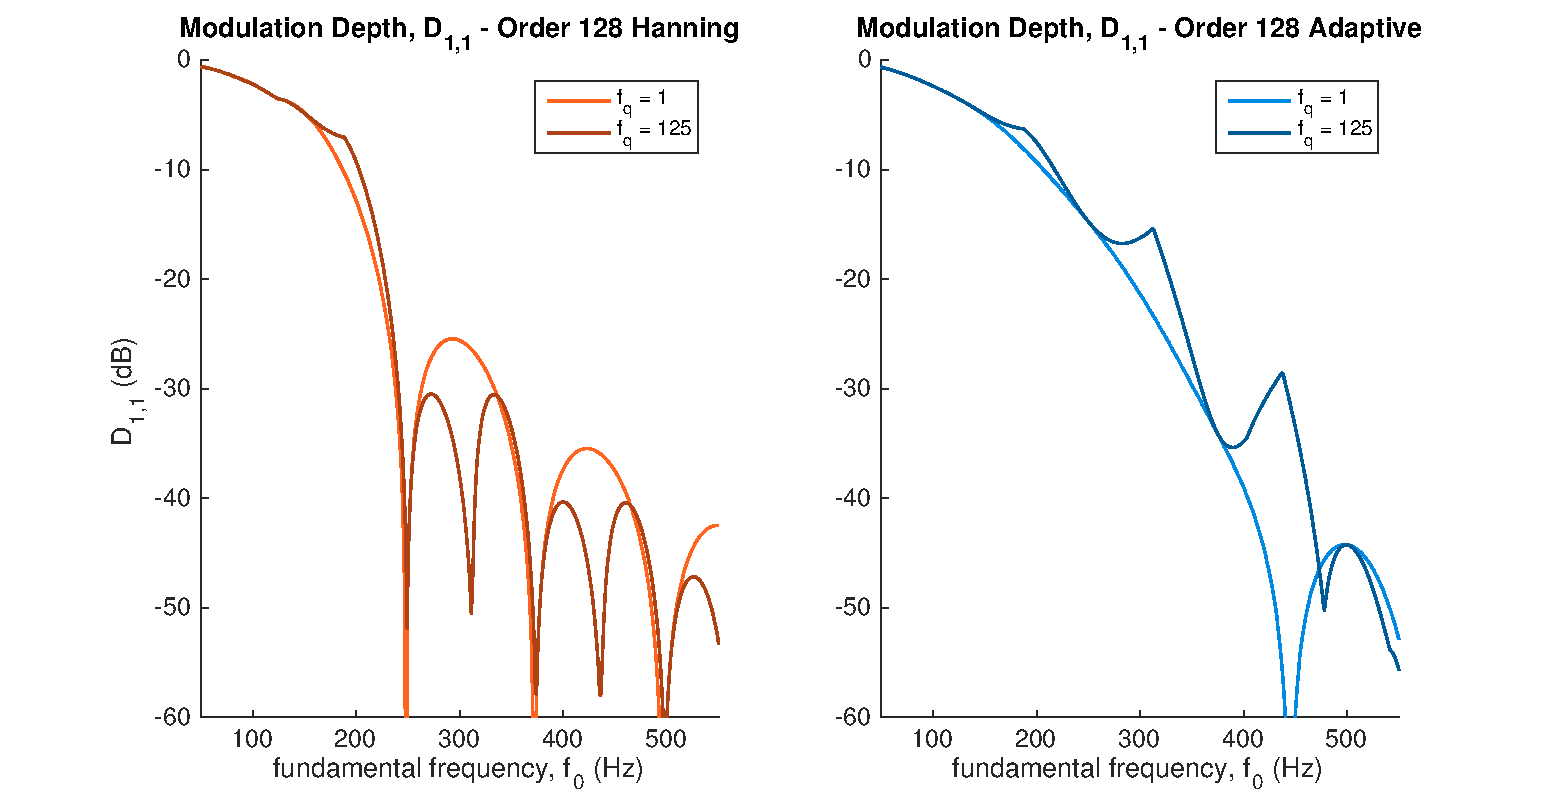
\includegraphics[width=1\textwidth]{d_ki_2}
    \caption{$D_{k,i}$ downshift quantization}\label{fig:d_ki_2}
\end{figure}

Provided no downshift quantization, ,odulation depth won't change as a function of $k$.  Figure~\ref{fig:d_ki_4} shows this variation, however it has minimal impact.

\begin{figure}[!ht]
  \centering
    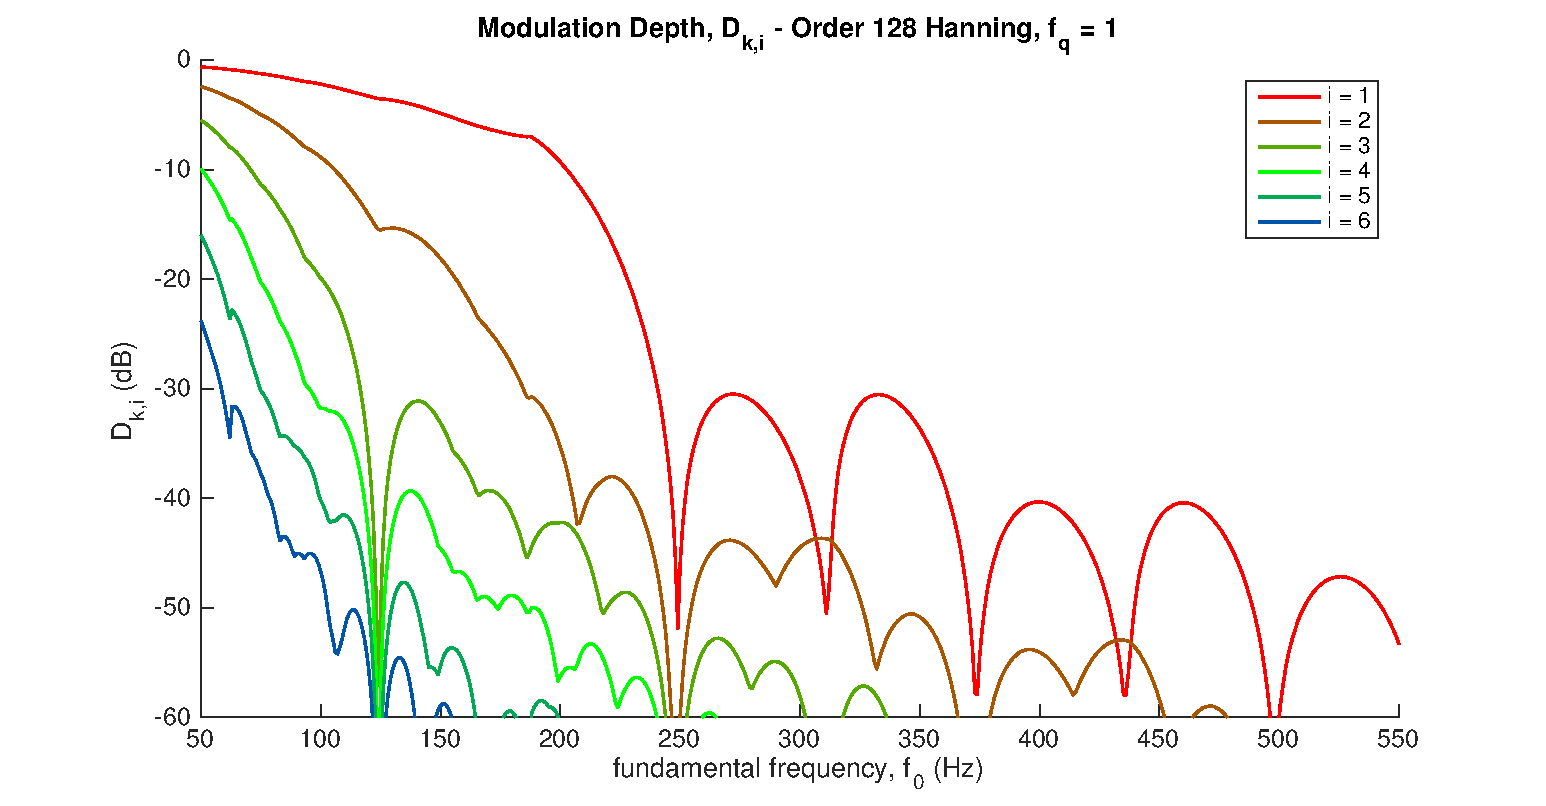
\includegraphics[width=1\textwidth]{d_ki_4}
    \caption{$D_{k,i}$ at rate of $iF_0$}\label{fig:d_ki_4}
\end{figure}

Recall $D_{k,i}$ is the modulation depth of the estimate of the $k$th harmonic at a rate of $iF_0$.  We should expect that as $i$ increases we move further away from baseband and our filter does a better job of eliminating modulations.  This is verified in figure~\ref{fig:d_ki_3}.

\begin{figure}[!ht]
  \centering
    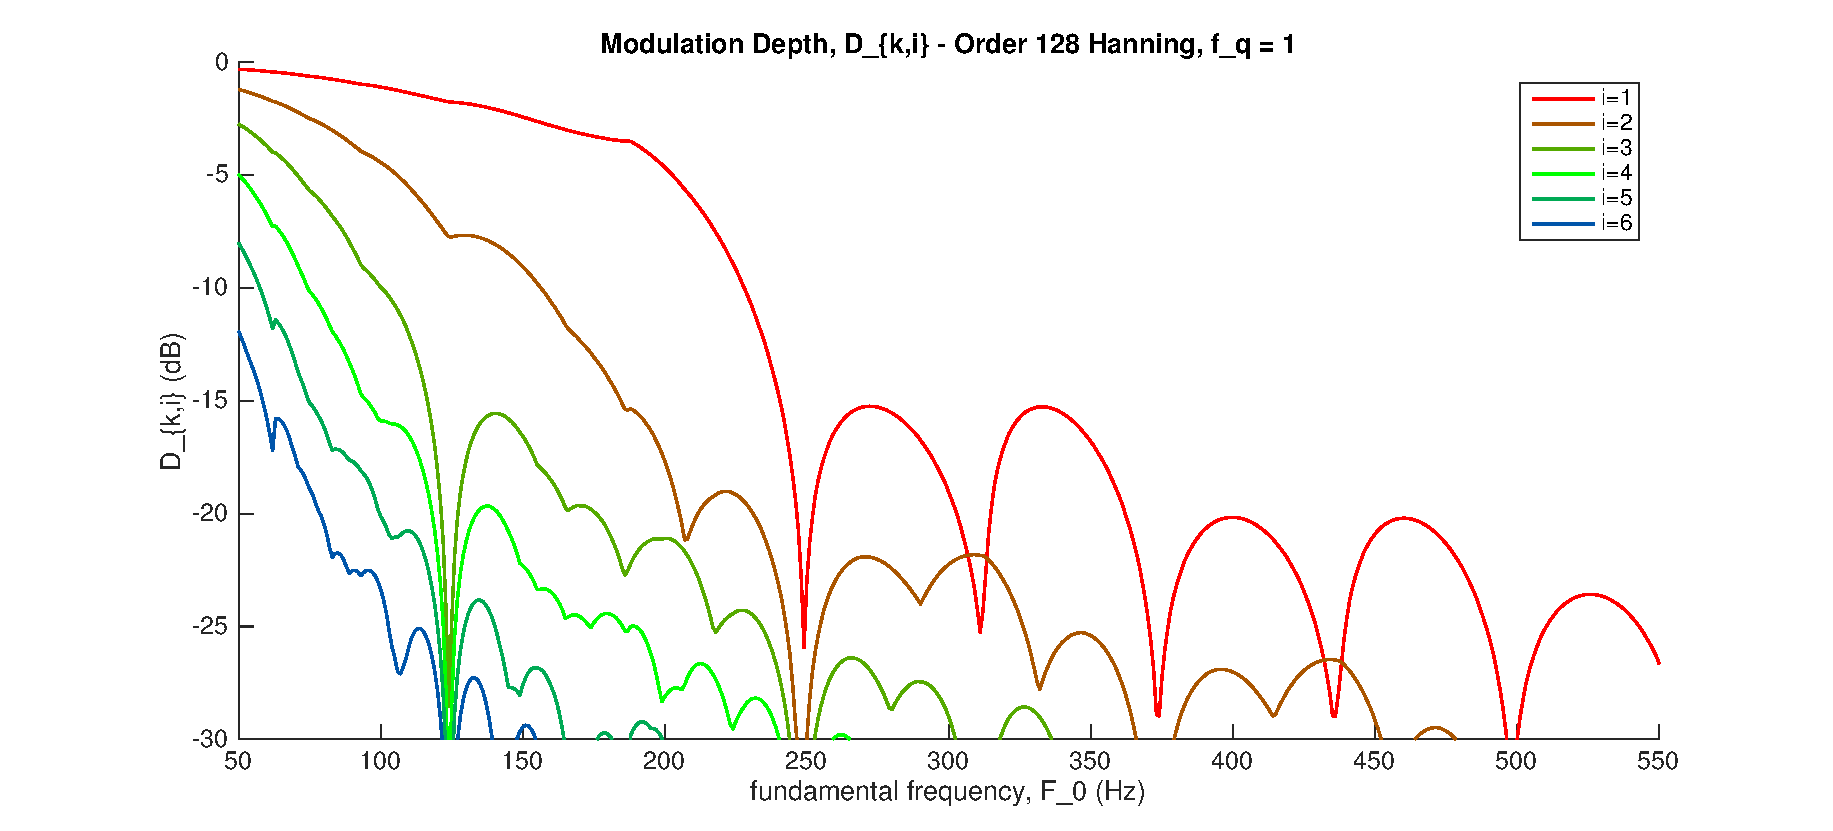
\includegraphics[width=1\textwidth]{d_ki_3}
    \caption{$D_{k,1}$ across harmonics}\label{fig:d_ki_3}
\end{figure}

This results suggest that $D_{k,1}$ is the most important measure, and that hanning and adaptive filter designs achieve approximately the same performance.  At low $F_0$ filter order plays a large roll in modulation depth.

Psychophysical studies have found that for reliable pitch discrimination amplitude-modulations of approximately 10\% to 40\% are required on average. [REF] %[pitch_ranking_strategy_compare].

\begin{align}
10\% \rightarrow D_{k,1} = -20 \mathrm{dB} \nonumber \\
40\% \rightarrow D_{k,1} = -8 \mathrm{dB} \nonumber
\end{align}


This implies that depending on the user:

- order 128 breaks down at $F_0\approx 240$ to $400$Hz

- order 256 breaks down at $F_0\approx 120$ to $200$Hz

- order 512 breaks down at $F_0\approx 60$ to $100$Hz

In the best case, order 512 is sufficient for all $F_0$.  In the worst case, order 128 will have artifacts across almost the entire $F_0$ range.


%``Previous CI psychophysical studies investigating the pitch of sinusoidal amplitude-modulated pulse trains have shown considerable variation between subjects in terms of the modulation depths required for reliable discrimination of pitch (McKay et al., 1995; Geurts and Wouters, 2001). On average, modulation depths ranging from 10\% to 40\% of the electrical dynamic range were required, although some subjects required depths of almost 100\%. Converting these values to the acoustic dynamic range coded by the sound processor, which for the Nucleus 24 system is typically 30 dB, indicates that modulation depths in the acoustic signal of approximately 3 to 12 dB are required on average.'' %[pitch_ranking_strategy_compare]

\subsection{Transients}

Time-responses are a bit more difficult to analyze, as we cannot use the standard dB measurements we are familiar with.  We will consider transient responses of the different filter designs and filter orders.

We start with the unit step response, shown in figure~\ref{fig:transient_1}.  Latency on the order of 15ms isn't of much concern.  The more important difference in the rise time.  The 10-90\% rise times are displayed in table~\ref{table:rise_times}.

The adaptive filters all have the same rise time at high enough $F_0$ however the lower order filters are fundamentally constrained on how slow the rise time can be.  The rectangular window is the worst of them all.

\begin{figure}[!ht]
  \centering
    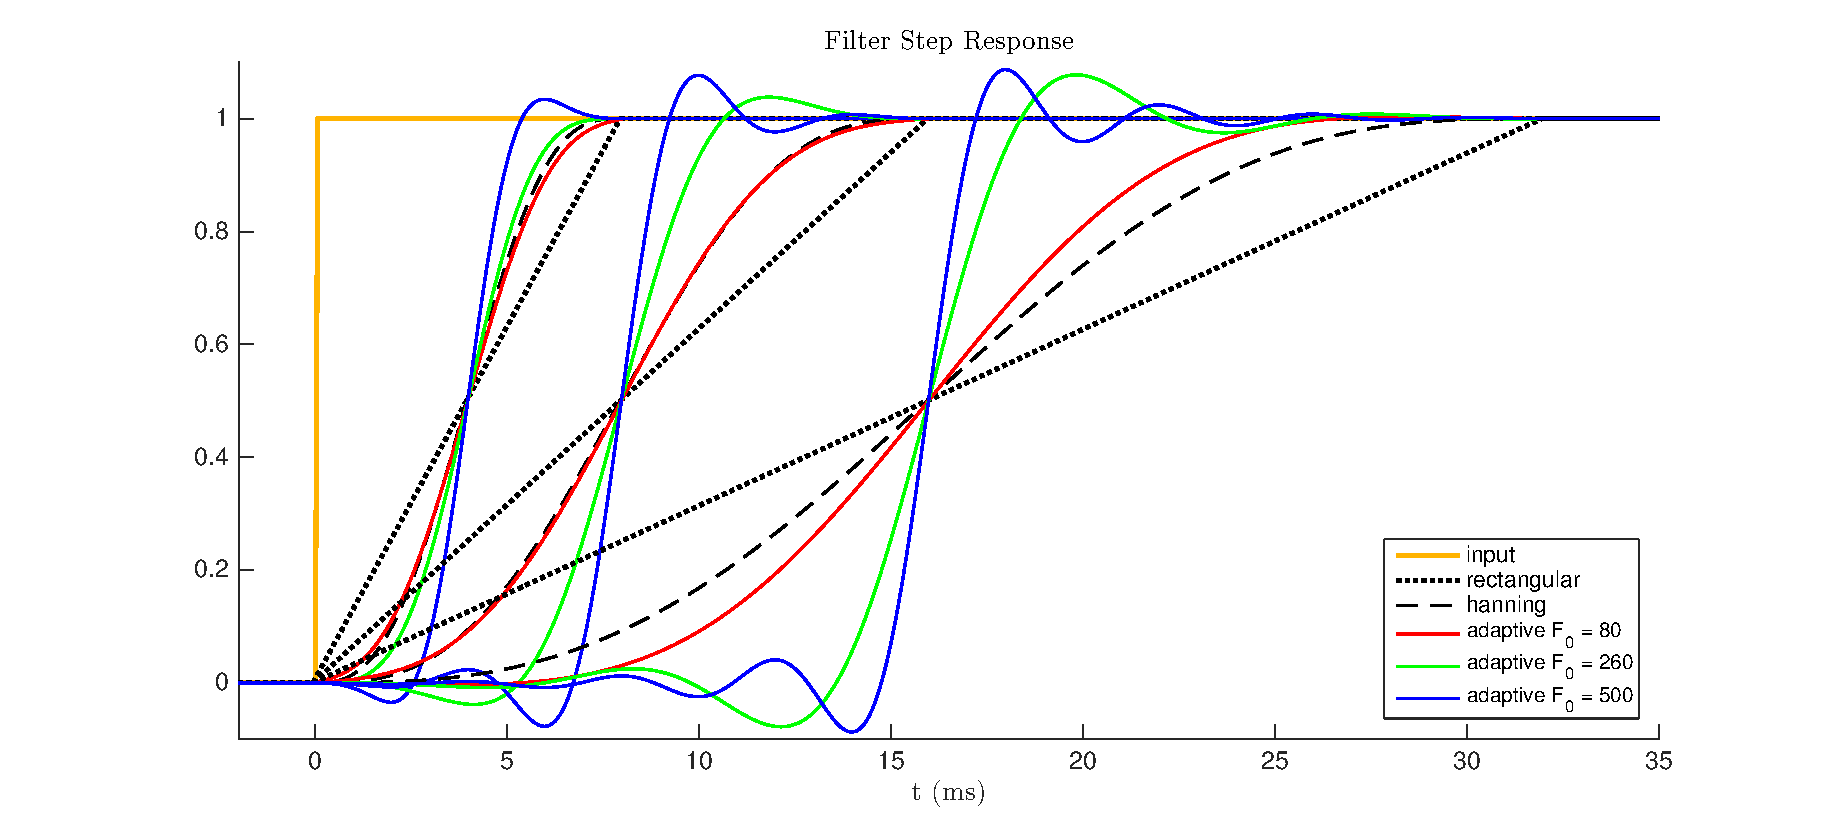
\includegraphics[width=1\textwidth]{transient_1}
    \caption{Transient Step Response, order = 128, 256, 512 (increasing order corresponds to longer reponse time)}\label{fig:transient_1}
\end{figure}

\begin{table}
\begin{center}
\begin{tabular}{| r | r | r | r | r | r |}
  \hline
    & rectangular & hanning & adaptive 80 & adaptive 260 & adaptive 500 \\ \hline
  \textbf{Order} & \multicolumn{5}{|c|}{\textbf{Rise Time (ms)}} \\ \hline
  128 & 7 & 4 & 4 & 3 & 2 \\ \hline
  256 & 13 & 8 & 8 & 4 & 2 \\ \hline
  512 & 26 & 16 & 12 & 4 & 2 \\ \hline
\end{tabular}
\end{center}
\caption{filter rise times}\label{table:rise_times}
\end{table}

An alternative view is shown in figure~\ref{fig:transient_2}.  For typical attack times in the range of 5-200ms and input to output change in attack time is plotted.

As mentioned in section~\ref{section:transients} humans hear transient changes in the log domain, and thus the axes are log scaled.

For the worse case, rectangular order 512, more than half the dynamic range is lost due to smearing.

\begin{figure}[!ht]
  \centering
    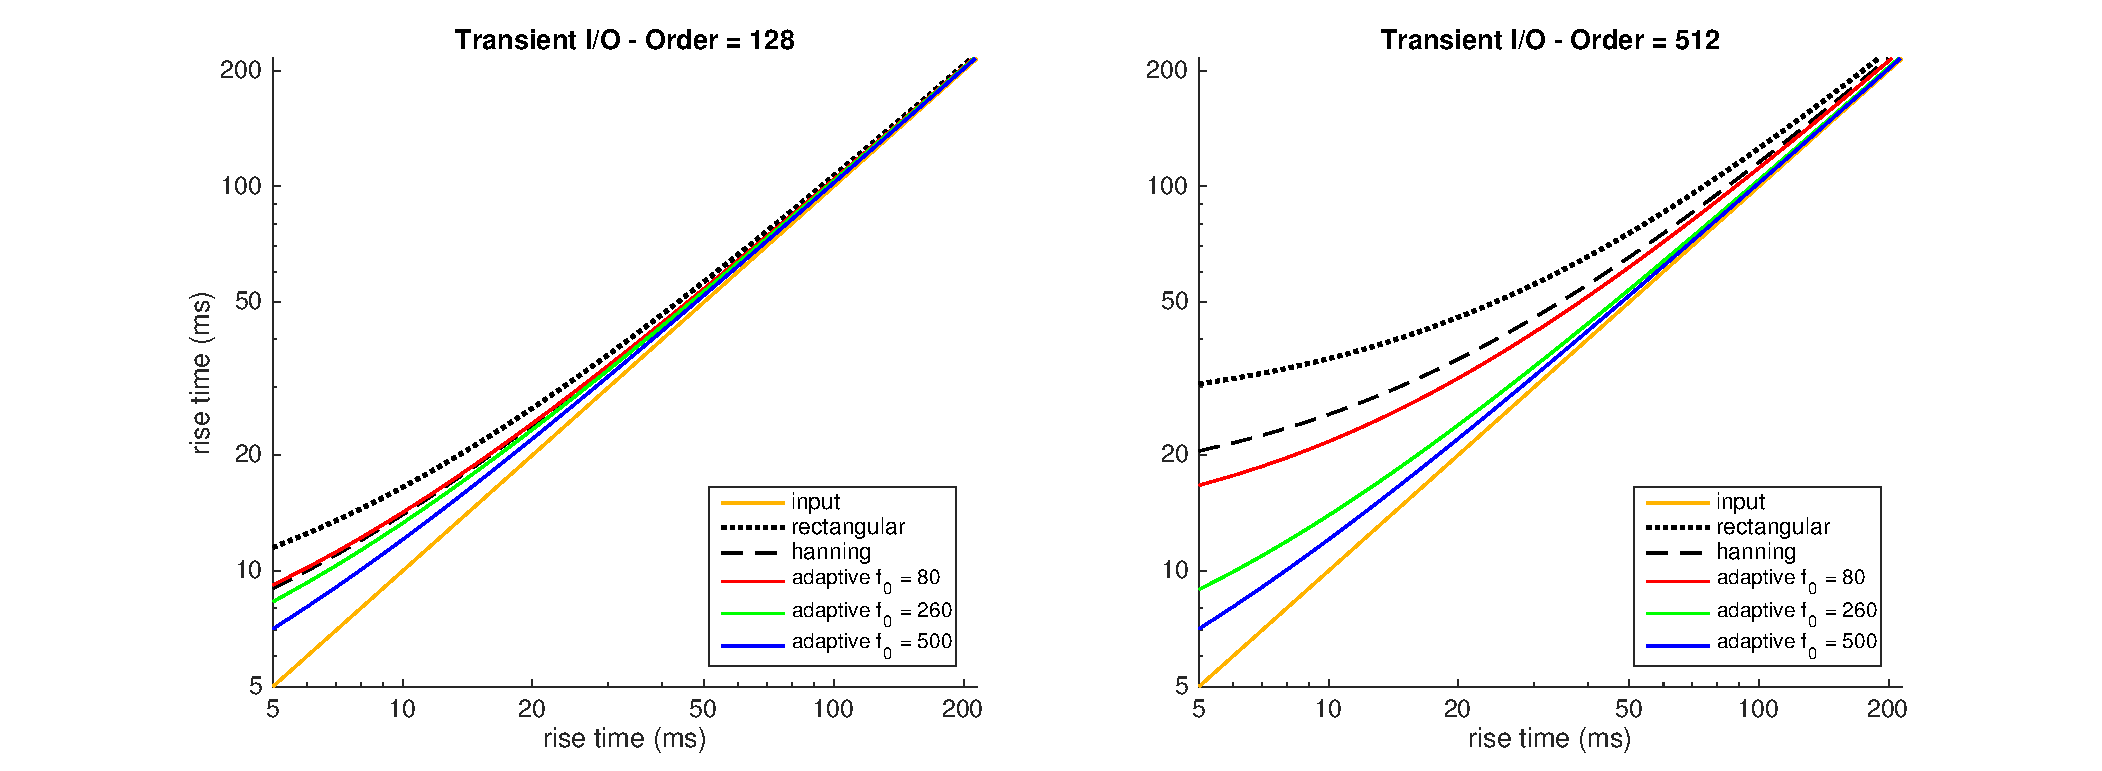
\includegraphics[width=1\textwidth]{transient_2}
    \caption{Transient Input/Output Change}\label{fig:transient_2}
\end{figure}

As a final perspective on transients, we consider typical instrument attack times.  Figure~\ref{fig:transient_3} shows the shifted attack times of twelve instruments typical attack times.  The vertical scale has no meaning, it is simply for visual clarity.

What's interesting is that on a log scale, the instruments generally bunch into two groups.  The slow attack-time group seems robust to the distortions of any of these filters.  On the other hand the fast-attack time instruments change dramatically.  For the narrow bandwidth 512 order filters, the smeared guitar output is closer in attack-time to an English horn than itself!

\begin{figure}[!ht]
  \centering
    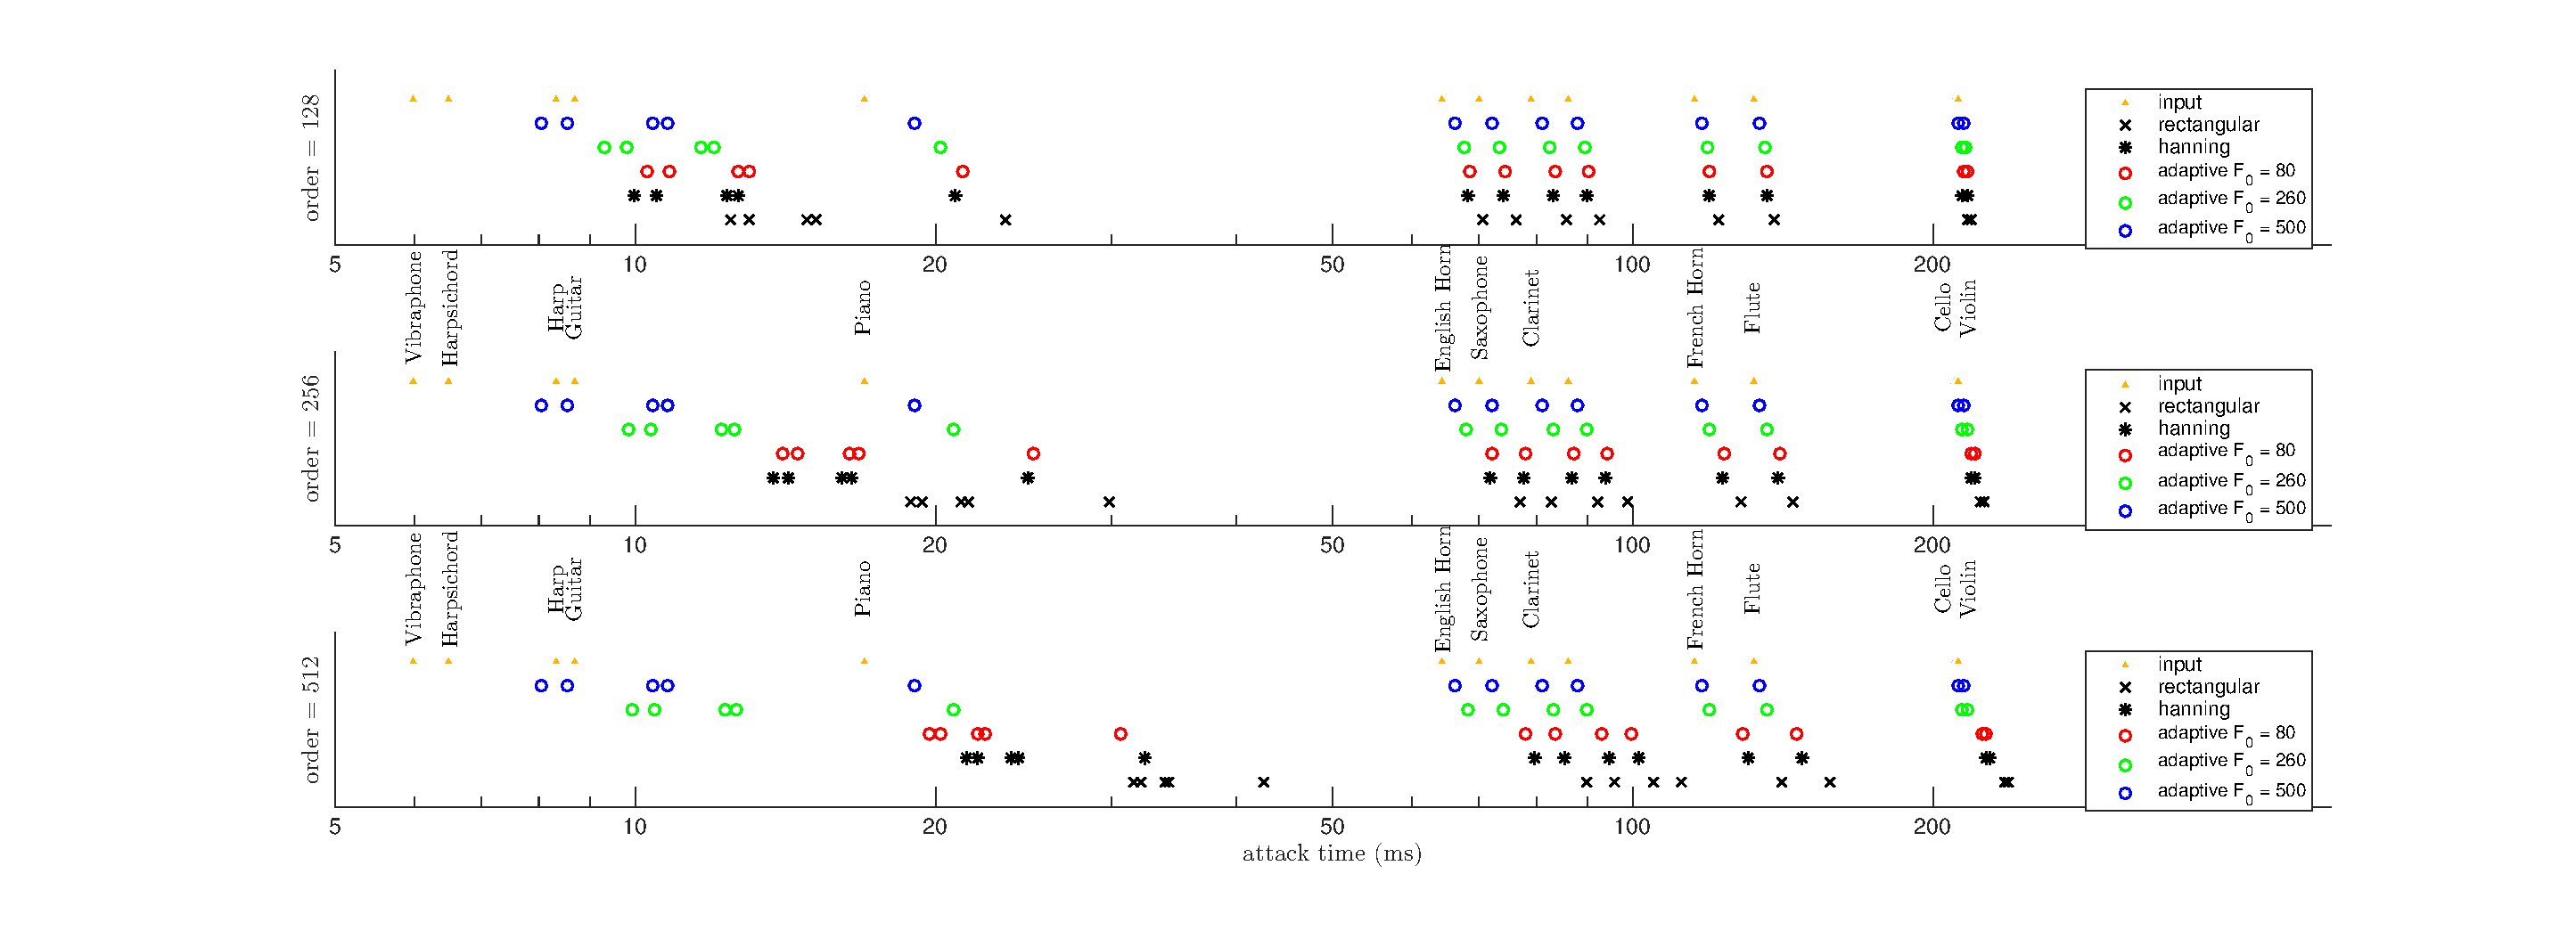
\includegraphics[width=1.2\textwidth]{transient_3}
    \caption{Transient Distortion for Common Instruments}\label{fig:transient_3}
\end{figure}

\clearpage

\subsection{Summary}

For the most part the hanning and adaptive filters outperformed rectangular.  The rectangular window's performance on modulation depth makes it essentially unusable.

For coherent gain we get a worst case of roughly -1.5dB.  It doesn't appear from our results to be an overly critical design consideration.

For harmonic SIR and modulation depth the critical performance variable was filter order.  To very loosely summarize, order 128 fails for $F_0 < 240$Hz, order 256 fails for $F_0 < 120$Hz and 512 does sufficiently well for the full range considered.

Downshift quantization also did not seem to play a prominent role.  This is in part affected by the restriction that quantization can't be worse than $F_s$ / filter order.

There is clearly an envelope bandwidth tradeoff, where the wider a filter is the less transients are smeared but the more the other harmonics interfere in the estimated envelope.

The sharp-cutoff order 512 filters smear the fast transients a significant amount, however the adaptive bandwidth filters seem to do well at smearing as little as possible while still achieving good performance on the other metrics.  This could be the best solution to the posed bandwidth tradeoff.

%harmonic bandwidth: what is it?  look at some waveforms and read some stuff.  maybe do this at the same time as transient times of instruments

\section{Non-ideal Pitch Estimators}

The critical assumption thus far has been accurate pitch estimates.  One problem to consider is error in the pitch estimator.  The other that we will consider is pitch estimator quantization.

We consider a specific pitch estimator that uses autocorrelation.  To summarize this method, an autocorrelation is performed on the windowed input.  A maxima is selected from this autocorrelation and the fundamental frequency is computed from the index of the maxima.

\begin{align}
R_{xx}[n,\tau] =& x_{windowed}[r] * x_{windowed}[-r] \\
\tilde{F}_0[n] =& F_s \Bigg[ \arg\max_\tau R_{xx}[n,\tau] \Bigg]^{-1}
\end{align}

This can be implemented efficiently using the fast-autocorrelation method

\begin{align}
R_{xx}[n,\tau] = \mathcal{F}^{-1}\Big\{X[n,k]X^*[n,k]\Big\}
\end{align}

Defining the FFT order as $N$, for this method the possible values of $F_0$ are 

\begin{align}
F_0 = \frac{F_s}{\tau}, \quad 1 \leq \tau \leq \frac{N}{2}
\end{align}

By then bounding the considered $F_0$ values to roughly 50-550Hz we can get better resolution by resampling the signal such that more values of $F_0$ fall within these bounds.

\begin{align}
max\Big(\frac{2Fs}{N}, 50\Big) \leq F_0 \leq min\Big(\frac{Fs}{2}, 550\Big)
\end{align}

Choosing $F_s$ is important, since the quantization of $F_0$ is not linearly spaced and becomes worse at higher values of $F_0$.

To be clear that this different sampling rate is only relevant to pitch estimation and not any of the other envelope extraction process, we define a new pitch estimator sampling rate, $F_{s,p}$.  Having $N$ as the filter orders we have previously considered we choose $F_{s,p}$ for maximal possibilities for $F_0$ within our region of interest.  The results are shown in table~\ref{table:f0_quantization}.

\begin{table}
\begin{center}
\begin{tabular}{| r | r | r | r | r | r |}
  \hline
  \textbf{Order ($N$)} & \textbf{$F_{s,p}$} &  \textbf{min $F_0$} & \textbf{max $F_0$} &  \textbf{best quantization} &  \textbf{worst quantization} \\ \hline
  128 & 4kHz & 63Hz & 500Hz & 1Hz & 56Hz \\ \hline
  256 & 8kHz & 63Hz & 533Hz & 1Hz & 33Hz \\ \hline
  512 & 16kHz & 63Hz & 533Hz & 1Hz & 17Hz \\ \hline
\end{tabular}
\end{center}
\caption{$F_0$ estimate quantization}\label{table:f0_quantization}
\end{table}

With this design each $N$ covers approximately the same range, however the high orders have 2 or 4 times as many samples as $N = 128$.  This is especially important at high values of $F_0$ where the quantization is the worst.

We revisit harmonic SIR and modulation depth with non-deal pitch estimates.  Downshift quantization is assumed: $f_q = \frac{F_s}{N}$.

\subsection{Harmonic SIR}

Harmonic SIR is visualized for two different filter design methods in figues~\ref{fig:pitch_sir_k_1} and ~\ref{fig:pitch_sir_k_2}.  The pitch quantization, which is worse for lower orders, causes harmonic SIR to degrade for higher harmonics.  This makes sense as the quantization error will be scaled by harmonic index $k$.

The hanning filter performs slightly at high $F_0$s bettter due to narrower filter bandwidth.  Depending on the desired performance, harmonic indices above a certain threshold will no longer provide accurate harmonic envelopes.  This threshold is slightly lower for adaptive filters than hanning filters and it is significantly lower for lower order filters.

\begin{figure}[!ht]
  \centering
    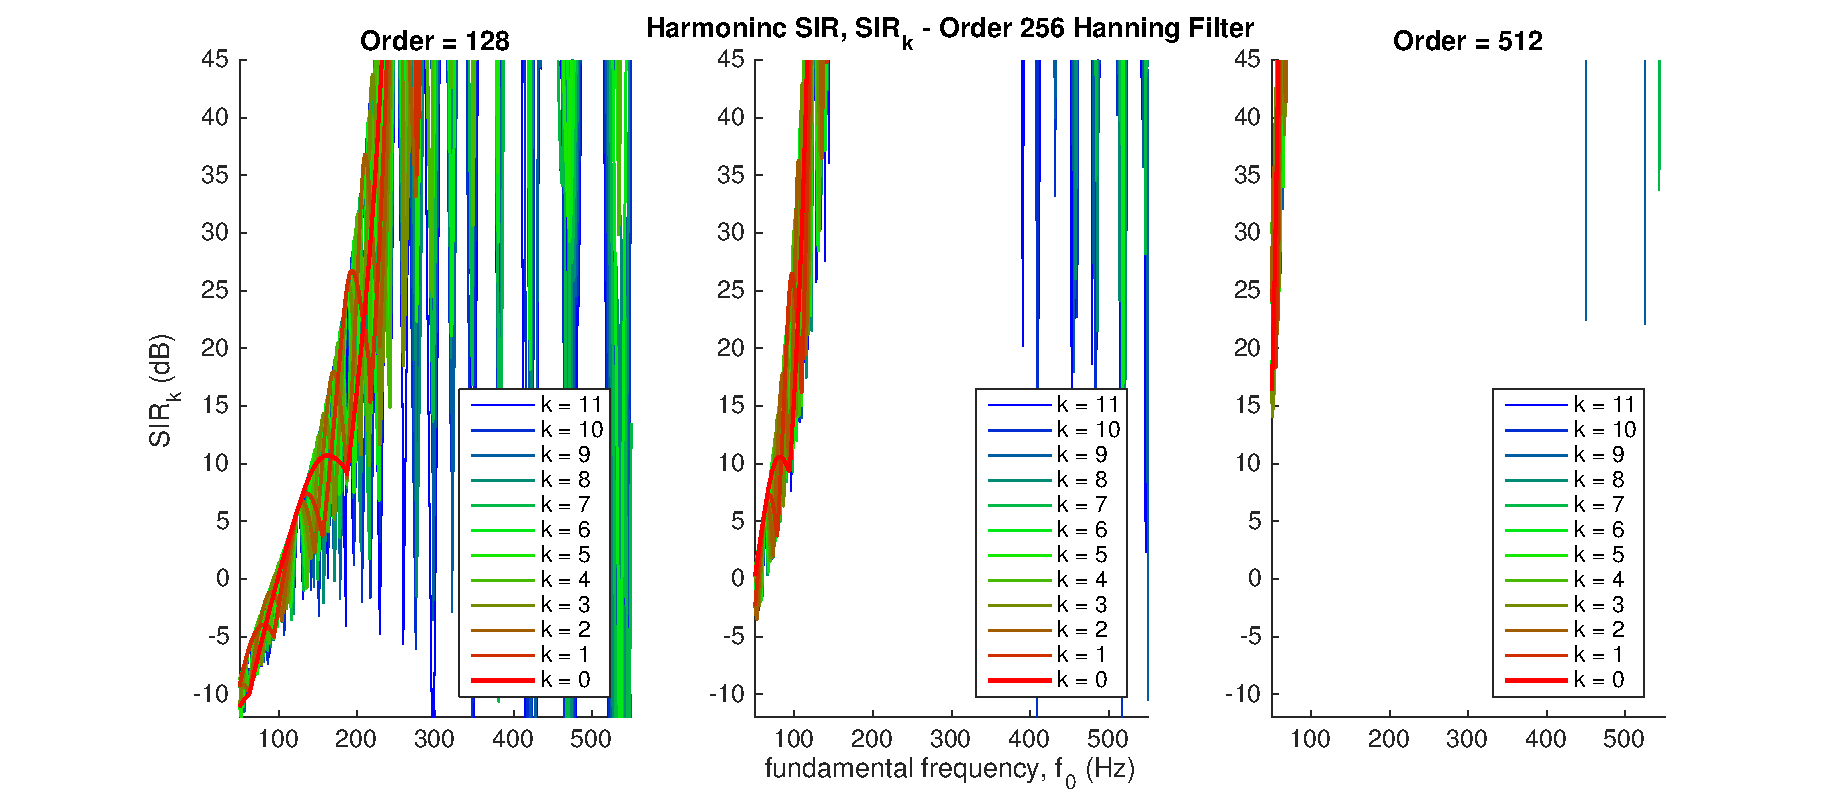
\includegraphics[width=1\textwidth]{pitch_sir_k_1}
    \caption{$SIR_k$, hanning filter and pitch estimate quantization}\label{fig:pitch_sir_k_1}
\end{figure}

\begin{figure}[!ht]
  \centering
    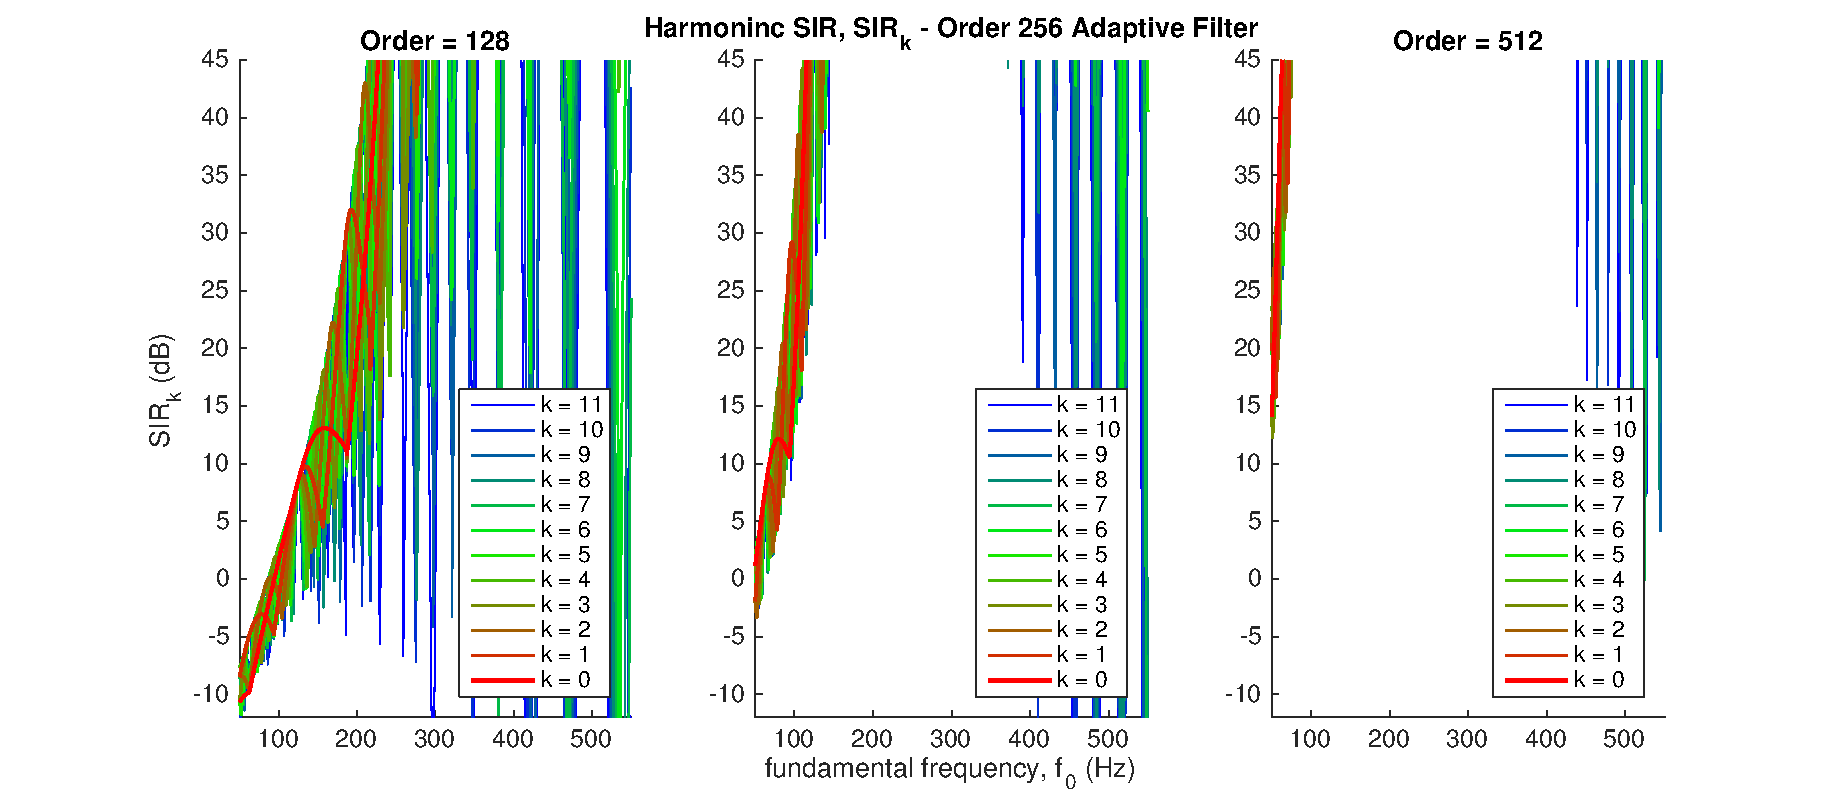
\includegraphics[width=1\textwidth]{pitch_sir_k_2}
    \caption{$SIR_k$, adaptive filter and pitch estimate quantization}\label{fig:pitch_sir_k_2}
\end{figure}

We now consider the same designs but with $\pm5$Hz pitch estimation error.  The worse case $SIR_k$ is shown for hanning filter in figure~\ref{fig:pitch_sir_k_1_error5} and for adaptive filter in figure~\ref{fig:pitch_sir_k_2_error5}.

The error degrades performance in two dimensions.  Similar to quantization error, the perfomance degrades proportional to $k$.  The other problem is at low values of $F_0$, where harmonics are more closely spaced.

We can take the right plot in figure~\ref{fig:pitch_sir_k_1_error5} as an example.  For the first 3 harmonics we get good harmonic SIRs for $F_0 > 80$Hz, however for $k = 3,4$ this increases to roughly $F_0 > 180$Hz and for even higher harmonics we never achieve satisfactory SIR.

\begin{figure}[!ht]
  \centering
    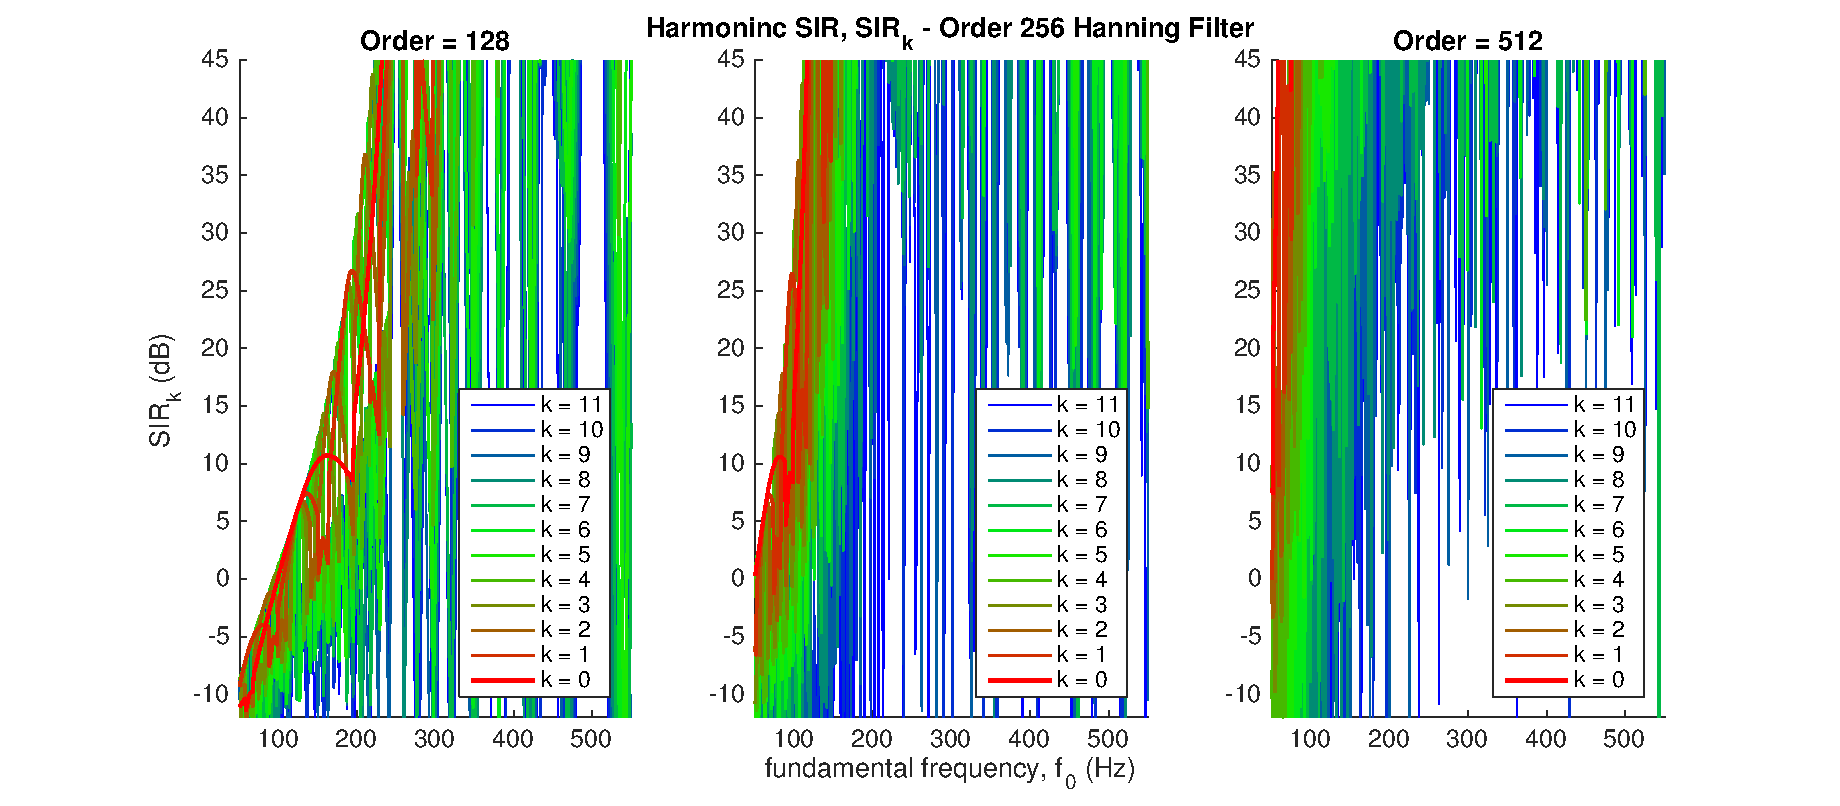
\includegraphics[width=1\textwidth]{pitch_sir_k_1_error5}
    \caption{$SIR_k$, hanning filter, pitch estimate quantization and $\pm5$Hz estimation error}\label{fig:pitch_sir_k_1_error5}
\end{figure}

\begin{figure}[!ht]
  \centering
    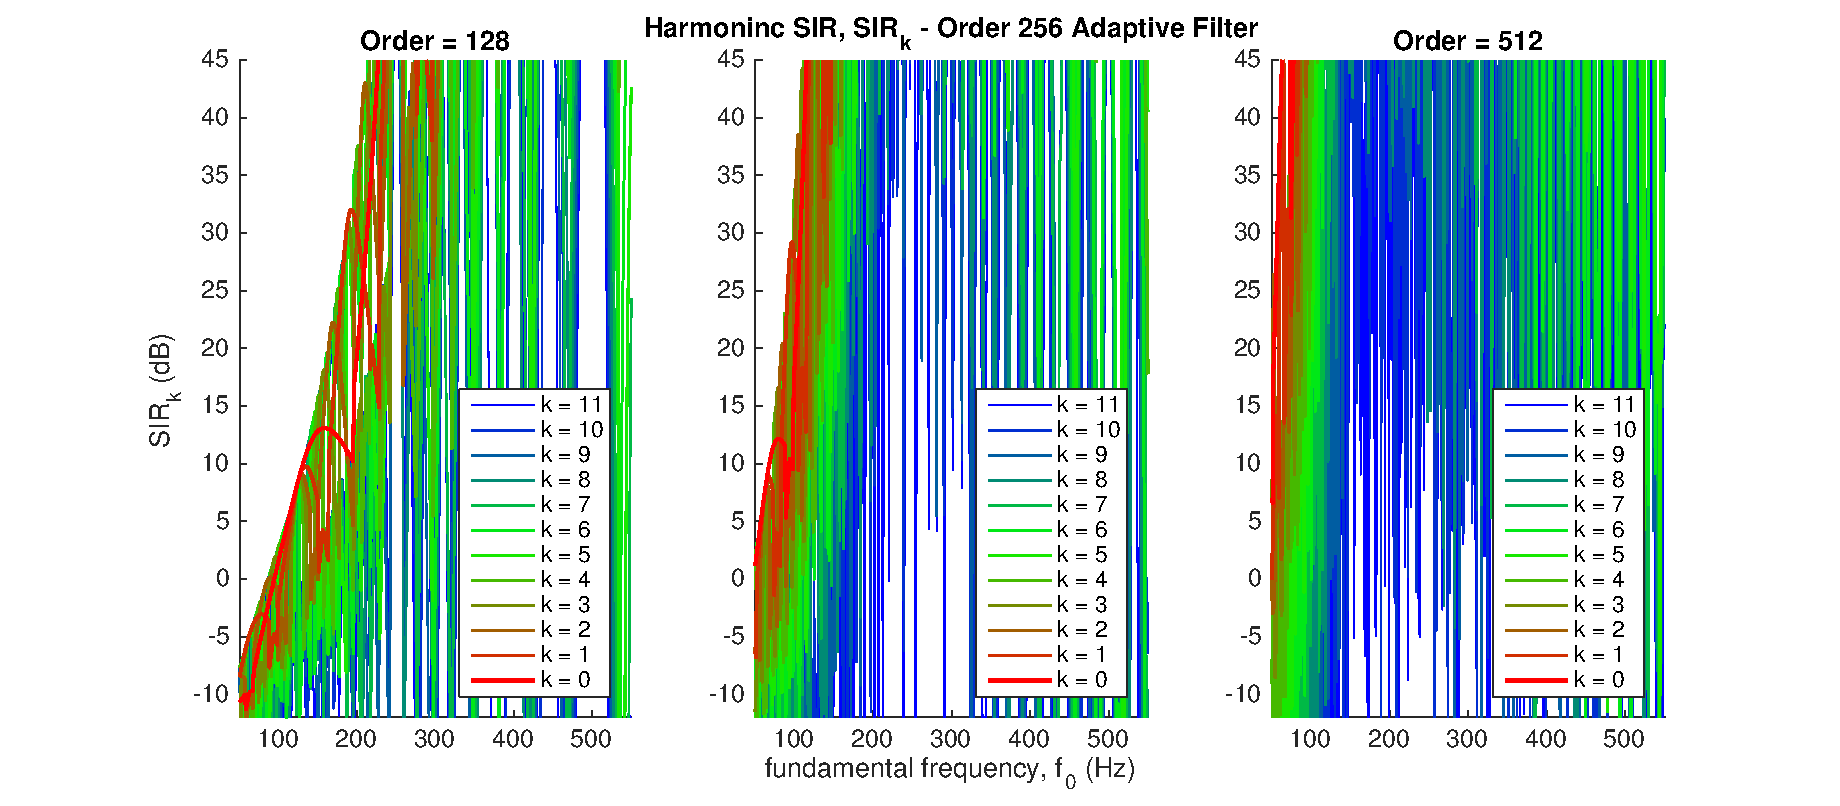
\includegraphics[width=1\textwidth]{pitch_sir_k_2_error5}
    \caption{$SIR_k$, adaptive filter, pitch estimate quantization and $\pm5$Hz estimation error}\label{fig:pitch_sir_k_2_error5}
\end{figure}

\clearpage

\subsection{Modulation Depth}

We repeat these same comparisons for modulation depth.  Looking at figure~\ref{fig:pitch_d_ki_1}, with hanning filter and pitch estimate quantization, high harmonics have very high modulations.  Around the 6th harmonic ($k = 5$) we start to see big spikes in modulation depth at high $F_0$.  Interestingly the same harmonics have poor performance regardless of $N$, however there is a far broader region of failure for lower $N$.

In  figure~\ref{fig:pitch_d_ki_2} we see much better performance for $N = 512$ in comparison to the hanning filer.  This is because despite having wider bandwidth at high $F_0$, the sidelobes are much lower than the hanning filter.  The first hanning sidelobe has a gain of -31dB, whereas for $F_0 = 500$Hz the adaptive filter has a first sidelobe gain of -56dB.

\begin{figure}[!ht]
  \centering
    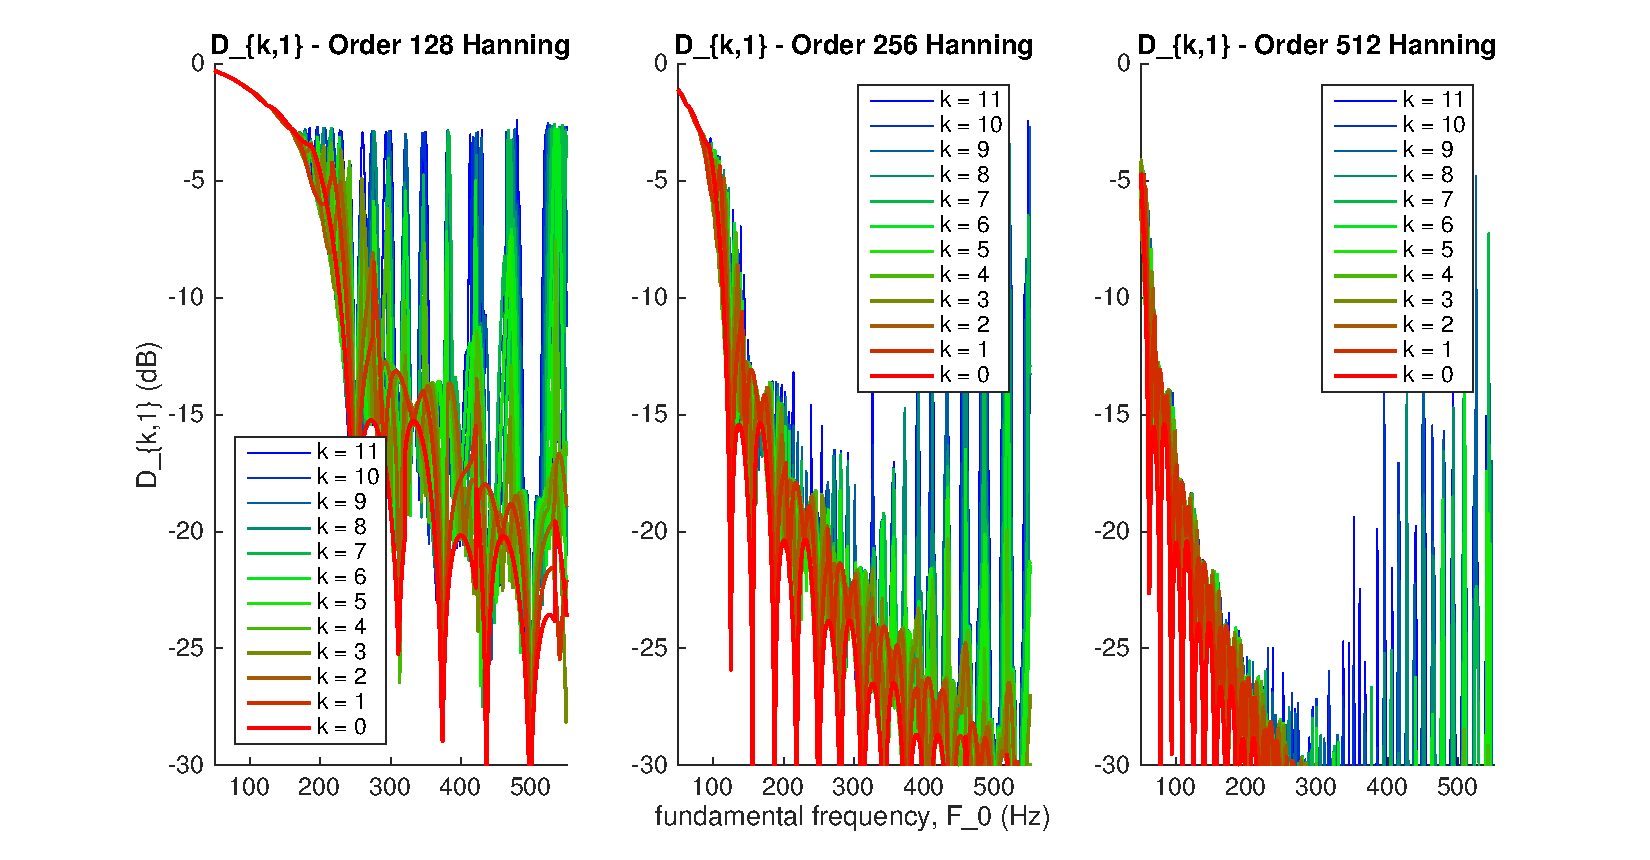
\includegraphics[width=1\textwidth]{pitch_d_ki_1}
    \caption{$D_{k,1}$, hanning filter and pitch estimate quantization}\label{fig:pitch_d_ki_1}
\end{figure}

\begin{figure}[!ht]
  \centering
    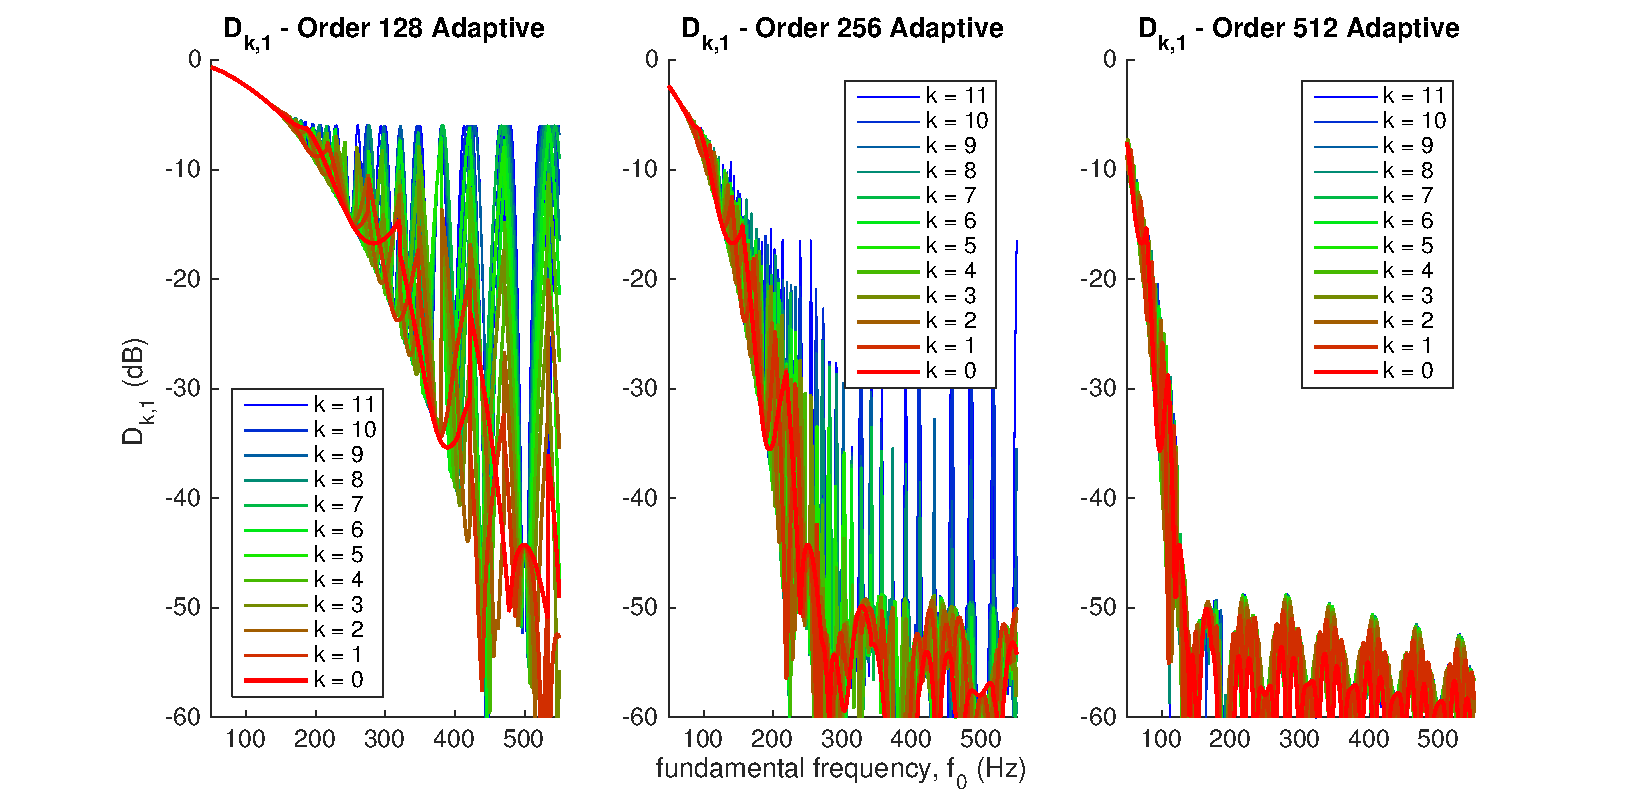
\includegraphics[width=1\textwidth]{pitch_d_ki_2}
    \caption{$D_{k,1}$, hanning filter and pitch estimate quantizationr}\label{fig:pitch_d_ki_2}
\end{figure}

Now considering $\pm5$Hz estimation error, we see from figures~\ref{fig:pitch_d_ki_1_error5} and \ref{fig:pitch_d_ki_2_error5} the same shift right where higher harmonics at low $F_0$ perform worse.  The adaptive order 512 filter performs the best, being very robust error.

\begin{figure}[!ht]
  \centering
    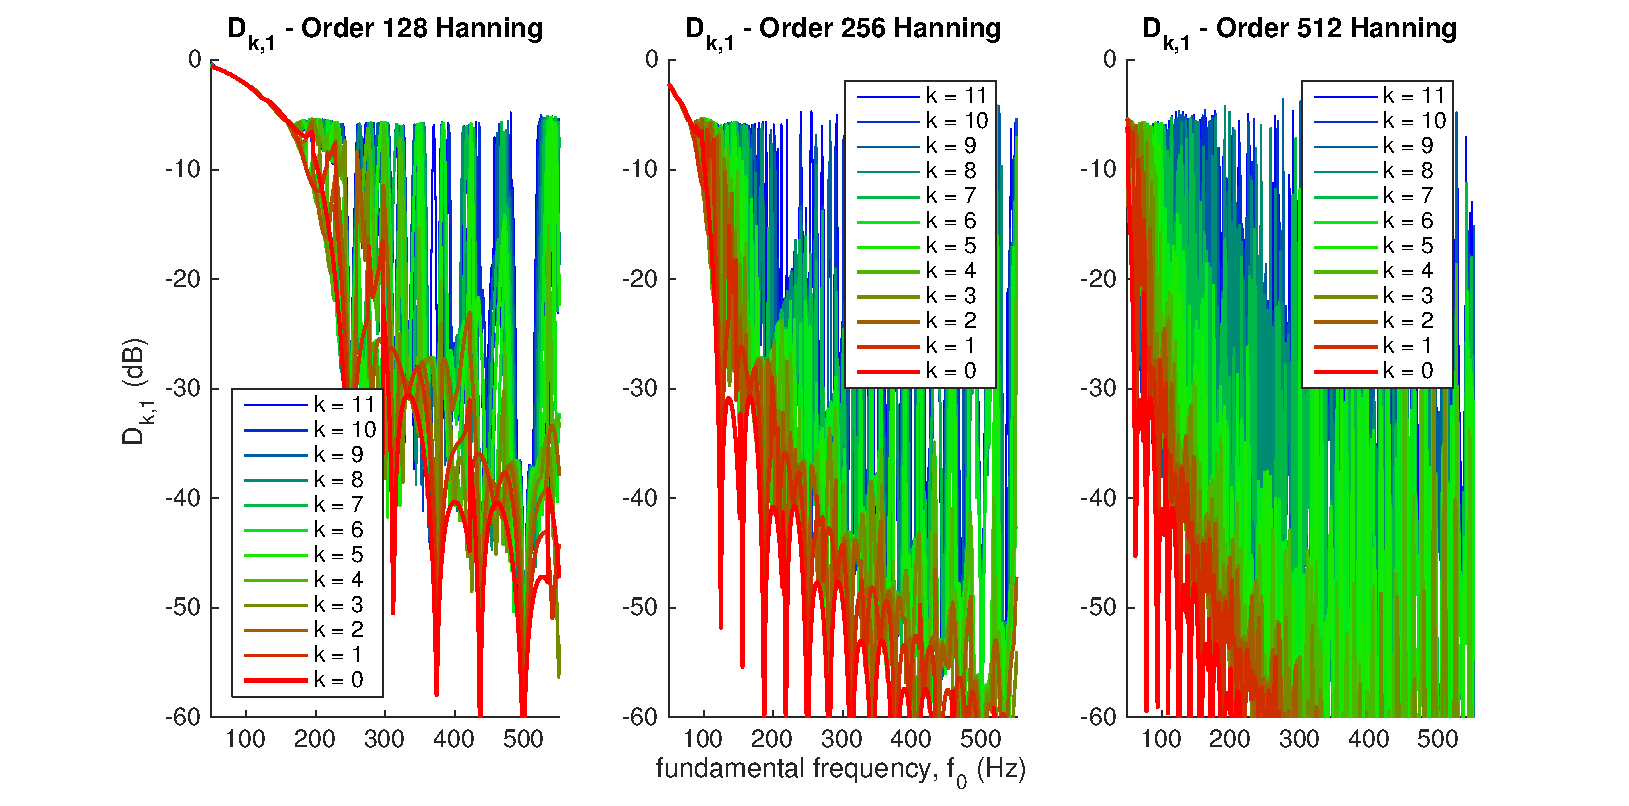
\includegraphics[width=1\textwidth]{pitch_d_ki_1_error5}
    \caption{$D_{k,1}$, hanning filter, pitch estimate quantization and $\pm5$Hz estimation error}\label{fig:pitch_d_ki_1_error5}
\end{figure}

\begin{figure}[!ht]
  \centering
    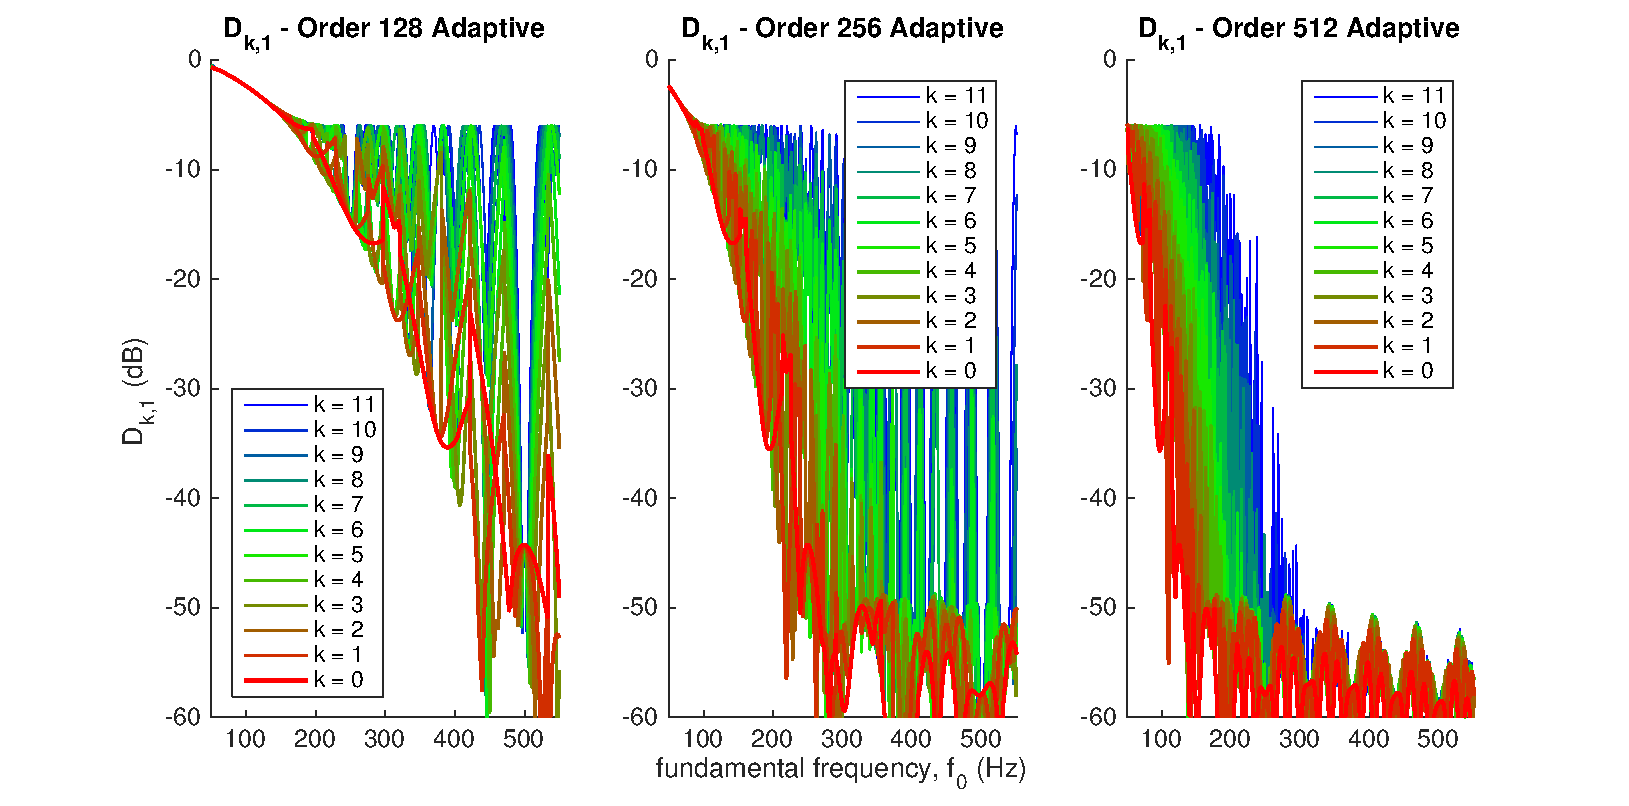
\includegraphics[width=1\textwidth]{pitch_d_ki_2_error5}
    \caption{$D_{k,1}$, hanning filter, pitch estimate quantization and $\pm5$Hz estimation error}\label{fig:pitch_d_ki_2_error5}
\end{figure}

Regardless of extraction method there will be a fundamental limit on performance as the pitch estimate becomes worse.  We see from all of the above example that performance degrades proportional to $k \times \mathrm{error} / F_0$.

\section{Mapping and Selection}

coherent harmonic processing is different from incoherent in two fundamental ways:

1) envelopes are extracted coherently to minimize distortions

2) only envelopes relating to harmonics are calculated, this frees 

Fixed Greenwood bands are determined offline, corresponding each electrode with a bandwidth.  The $N$ envelopes are then mapped to electrodes by finding the greenwood bands each harmonic falls within.

Two general solutions

1) Adaptive (select loudest)

similar to ACE, we can choose the loudest channels.  This suffers from stability issues.  We can apply another heuristic to stabilize the decision based on consistency of signal energy and fundamental frequency

2) Fixed

stable, each option suffers from missing key harmonics to the signal

lowest channels will imply no high frequency energy, which could be bad for unvoiced signals

other relationships such as odd harmonics or prime numbered harmonics could miss harmonics critical to timbre perception.

fixed is more computationally efficient!


how to allocate harmonics to channels: combine, select 1st, select largest

hint at hybrid via failure to represent of selection options to represent the high channels well.

how to choose channels, largest vs fixed

heuristics on both!

Because we have isolated individual harmonic envelopes there is no issue of signal energy falling in between channels.

Another bonus to HSSE is that we may add a simple heuristic to maintain channel mapping stability.  For example, if F0 has not varied significantly since the previous frame, we can allocate to the same channels to avoid unnecessary switching between channels induced by vibrato or inaccuracies in pitch estimation.


%\section{Subject Tests (maybe)}

%All methods: order 128 hanning, $f_q = 125$Hz
%ACE, Hybrid, HSSE (1-8, all-even, odd)
%show oscilloscope figures?
%or maybe make simulations that compare 128, 256, 512 and adaptive vs hanning

\section{Implementation Considerations}

\subsection{Carrier Synthesis}

what waveform?

raised vs rectified, (raised seems better)

cite that 4-waveform paper

Swanson thesis: ``A high-rate pulse train, modulated on and off at frequency F0, had a higher pitch than a train of pulses at the rate of F0. If amplitude modulation of high-rate pulse trains is to be used to convey pitch, then the shape of the modulating waveform is important: a half-wave shape is better than a square-wave (on-off) shape.''

\subsection{Pitch Estimator}

importance of a good pitch estimator

improving pitch estimator

haven't yet mentioned octave errors

\subsection{Adaptive Filters using FFT}

...

improved filter quantization using interpolation

\subsection{Efficient FFT Interpolation Algorithm}

FFT with changeable window, and interpolate

Can this be done with different filter as function of F0?
We probably need to design the filters such that they pass reconstruction requirements

Is the actual equation just a sinc function times a phase shift?!

READ THIS: [An Intelligent FFT-Analyzer with Harmonic Interference Effect Correction and Uncertainty Evaluation]

\subsection{Stimulation Rate}

`` it was important not to change other
12 HWR strategy take-home study 224
aspects of the strategy, in particular, stimulation rate. It would not be a fair comparison to trial HWR at 1800 pps against ACE at 900 pps, as the increased stimulation rate in itself could affect performance. A higher rate could potentially represent amplitude modulation cues more faithfully (McKay et al. 1994). Conversely, there is evidence that sensitivity to temporal modulation is worse at higher rates (Galvin and Fu 2005).''
[swanson thesis]

\subsection{encoding transients}

explicit transient encoding using transient detectors  [find a vocoder ref]

\subsection{Hybrid Methods}

Most everything so far has assumed the signal has an $F_0$, what if it doesn't?  What if it is well outside the boundaries of $F_0$?  What about polyphonic music?  What about SNRs below what is needed for accurate $F_0$ estimation.

hybrid considerations

1) to achieve harmonic and inharmonic at same time

2) to better model the critical bands in the cochlea

maybe narrower filters could improve SiN, this was not investigated

effective information bandwidth: should I really get into this?
From the theoretical standpoint, envelope extraction is exactly the same in ACE and F0mod.  In implementation ACE typically uses a lower order FFT.  In [laneau] the authors consider 128-point for ACE and 512-point for F0mod and both will be considered here.
        with respect to bandwidth we actually have to different things, filter bandwidth and effective information bandwidth.  The former is obvious, the later refers to what frequencies are encoded on a electrode channel.  If multiple narrowband filters are somehow combined on the same channel, they may have the same information bandwidth as one wideband filter.
        
soft decisions (e-Tone)

``bowed string tones are inharmonic during both their attack and decay (Beauchamp, 1974)''

\section{Summary}



% ========== Chapter 5

\chapter{Conclusion}\label{ch:conclusion}

\section{Summary}

\section{Future Work}


%
% ==========   Bibliography
%
\nocite{*}   % include everything in the uwthesis.bib file
\bibliographystyle{plain}
\bibliography{ganter_thesis}
%
% ==========   Appendices
%
\appendix
\raggedbottom\sloppy
 
% ========== Appendix A

\chapter{Derivations}

%check appendix code 810982374981u23h

\begin{align}
\phi_0[n + r] =& \phi_0[n] + 2\pi \frac{F_0[n]}{F_s}r, \quad 0 \leq r < N \\
m_{k,harmonic}[n] =& \Bigg| x[n] e^{-jk\phi_0 [n]} *  \frac{1}{Nw[0]} w[-n] \Bigg| \nonumber \\
=& \frac{1}{Nw[0]} \Bigg| \sum_{r = -\infty}^\infty x[n - r] e^{-jk\phi_0 [n-r]} w[-r] \Bigg| \nonumber \\
\textrm{Let} \quad r' = -r \nonumber \\
=& \frac{1}{Nw[0]} \Bigg| \sum_{r' = 0}^{N-1} x[n + r'] e^{-jk\phi_0 [n + r']} w[r'] \Bigg|  \nonumber \\
=& \frac{1}{Nw[0]} \Bigg| e^{-jk \phi_0[n]} \sum_{r' = 0}^{N-1} x[n + r'] e^{-j \frac{2\pi F_0[n]}{F_s}kr'} w[r'] \Bigg| \nonumber \\
=& \frac{1}{Nw[0]} \Bigg| e^{-jk \Big(\phi_0[n] - \frac{2\pi F_0[n]}{F_s}n \Big)} \Bigg[ e^{-j \frac{2\pi F_0[n]}{F_s}kn} \sum_{r' = 0}^{N-1} x[n + r'] w[r'] e^{-j \frac{2\pi F_0[n]}{F_s}kr'} \Bigg] \Bigg| \nonumber \\
=& \frac{1}{Nw[0]} \Bigg| X\Big[n, \frac{N}{1} \frac{F_0[n]}{F_s} k \Big) \Bigg| \nonumber \\
\label{eq:harmonic-to-stft}
=& \frac{1}{Nw[0]} \Bigg| X\Big[n, \lambda[n]k\Big) \Bigg|
\end{align}

\vita{Tyler Ganter grew up in upstate New York, where the long cold winters inspired him to pick up guitar. While pursuing a BSEE at the University at Buffalo he took an interest computer programming, which he decided to minor in.  Through a continued interest in mathematics, software and music he found himself at home in the field of audio digital signal processing.  The desire to delve deeper into this field has led him to study at the University of Washington.}

\end{document}
